\documentclass[a4paper]{book}
\usepackage{makeidx}
\usepackage{graphicx}
\usepackage{multicol}
\usepackage{float}
\usepackage{listings}
\usepackage{color}
\usepackage{ifthen}
\usepackage[table]{xcolor}
\usepackage{textcomp}
\usepackage{alltt}
\usepackage{ifpdf}
\ifpdf
\usepackage[pdftex,
            pagebackref=true,
            colorlinks=true,
            linkcolor=blue,
            unicode
           ]{hyperref}
\else
\usepackage[ps2pdf,
            pagebackref=true,
            colorlinks=true,
            linkcolor=blue,
            unicode
           ]{hyperref}
\usepackage{pspicture}
\fi
\usepackage[utf8]{inputenc}
\usepackage{mathptmx}
\usepackage[scaled=.90]{helvet}
\usepackage{courier}
\usepackage{sectsty}
\usepackage[titles]{tocloft}
\usepackage{doxygen}
\lstset{language=C++,inputencoding=utf8,basicstyle=\footnotesize,breaklines=true,breakatwhitespace=true,tabsize=8,numbers=left }
\makeindex
\setcounter{tocdepth}{3}
\renewcommand{\footrulewidth}{0.4pt}
\renewcommand{\familydefault}{\sfdefault}
\begin{document}
\hypersetup{pageanchor=false}
\begin{titlepage}
\vspace*{7cm}
\begin{center}
{\Large ComPWA }\\
\vspace*{1cm}
{\large Generated by Doxygen 1.7.4}\\
\vspace*{0.5cm}
{\small Tue Nov 13 2012 16:02:16}\\
\end{center}
\end{titlepage}
\clearemptydoublepage
\pagenumbering{roman}
\tableofcontents
\clearemptydoublepage
\pagenumbering{arabic}
\hypersetup{pageanchor=true}
\chapter{Namespace Index}
\section{Namespace List}
Here is a list of all namespaces with brief descriptions:\begin{DoxyCompactList}
\item\contentsline{section}{\hyperlink{namespaceGem}{Gem} }{\pageref{df/d00/namespaceGem}}{}
\item\contentsline{section}{\hyperlink{namespaceGem_1_1Geneva}{Gem::Geneva} }{\pageref{db/de9/namespaceGem_1_1Geneva}}{}
\item\contentsline{section}{\hyperlink{namespaceROOT}{ROOT} }{\pageref{d0/d10/namespaceROOT}}{}
\item\contentsline{section}{\hyperlink{namespaceROOT_1_1Minuit2}{ROOT::Minuit2} }{\pageref{d6/d3a/namespaceROOT_1_1Minuit2}}{}
\end{DoxyCompactList}

\chapter{Class Index}
\section{Class Hierarchy}
This inheritance list is sorted roughly, but not completely, alphabetically:\begin{DoxyCompactList}
\item \contentsline{section}{DIFBase}{\pageref{d9/db5/classDIFBase}}{}
\begin{DoxyCompactList}
\item \contentsline{section}{DIFRootReader}{\pageref{dc/ddc/classDIFRootReader}}{}
\end{DoxyCompactList}
\item \contentsline{section}{GArgumentParser}{\pageref{d0/d39/classGArgumentParser}}{}
\item \contentsline{section}{Gem::Geneva::GStartIndividual}{\pageref{dd/d14/classGem_1_1Geneva_1_1GStartIndividual}}{}
\item \contentsline{section}{GStartIndividual}{\pageref{dd/d33/classGStartIndividual}}{}
\item \contentsline{section}{OIFBase}{\pageref{d0/d31/classOIFBase}}{}
\begin{DoxyCompactList}
\item \contentsline{section}{OIFGeneva}{\pageref{d4/dce/classOIFGeneva}}{}
\item \contentsline{section}{OIFMinuit}{\pageref{d5/db7/classOIFMinuit}}{}
\end{DoxyCompactList}
\item \contentsline{section}{OIFData}{\pageref{d1/d4f/classOIFData}}{}
\begin{DoxyCompactList}
\item \contentsline{section}{EIFBase}{\pageref{df/d13/classEIFBase}}{}
\begin{DoxyCompactList}
\item \contentsline{section}{EIFChiOneD}{\pageref{db/d1d/classEIFChiOneD}}{}
\end{DoxyCompactList}
\item \contentsline{section}{PolyFit}{\pageref{de/d89/classPolyFit}}{}
\end{DoxyCompactList}
\item \contentsline{section}{OIFMinuitFcn}{\pageref{d5/d19/classOIFMinuitFcn}}{}
\item \contentsline{section}{ROOT::Minuit2::OIFMinuitFcn}{\pageref{d3/dc7/classROOT_1_1Minuit2_1_1OIFMinuitFcn}}{}
\item \contentsline{section}{PIFBase}{\pageref{d5/d3f/classPIFBase}}{}
\begin{DoxyCompactList}
\item \contentsline{section}{PIFBW}{\pageref{d8/d58/classPIFBW}}{}
\end{DoxyCompactList}
\item \contentsline{section}{PWAEvent}{\pageref{dc/d66/classPWAEvent}}{}
\item \contentsline{section}{PWAParameter$<$ T $>$}{\pageref{d2/d41/classPWAParameter}}{}
\item \contentsline{section}{PWAParticle}{\pageref{d9/dcb/classPWAParticle}}{}
\end{DoxyCompactList}

\chapter{Class Index}
\section{Class List}
Here are the classes, structs, unions and interfaces with brief descriptions:\begin{DoxyCompactList}
\item\contentsline{section}{\hyperlink{classDIFBase}{DIFBase} (Data Interface Base-\/Class )}{\pageref{d9/db5/classDIFBase}}{}
\item\contentsline{section}{\hyperlink{classDIFRootReader}{DIFRootReader} (Reader for data in Root-\/files )}{\pageref{dc/ddc/classDIFRootReader}}{}
\item\contentsline{section}{\hyperlink{classEIFBase}{EIFBase} (Estimator Interface Base-\/Class )}{\pageref{df/d13/classEIFBase}}{}
\item\contentsline{section}{\hyperlink{classEIFChiOneD}{EIFChiOneD} (Simple $\chi^{2}$-\/Estimator )}{\pageref{db/d1d/classEIFChiOneD}}{}
\item\contentsline{section}{\hyperlink{classGArgumentParser}{GArgumentParser} (Geneva Argument Parser )}{\pageref{d0/d39/classGArgumentParser}}{}
\item\contentsline{section}{\hyperlink{classGStartIndividual}{GStartIndividual} (Geneva individual for optimization )}{\pageref{dd/d33/classGStartIndividual}}{}
\item\contentsline{section}{\hyperlink{classGem_1_1Geneva_1_1GStartIndividual}{Gem::Geneva::GStartIndividual} }{\pageref{dd/d14/classGem_1_1Geneva_1_1GStartIndividual}}{}
\item\contentsline{section}{\hyperlink{classOIFBase}{OIFBase} (Optimizer Interface Base-\/Class )}{\pageref{d0/d31/classOIFBase}}{}
\item\contentsline{section}{\hyperlink{classOIFData}{OIFData} (Optimizer Data Base-\/Class )}{\pageref{d1/d4f/classOIFData}}{}
\item\contentsline{section}{\hyperlink{classOIFGeneva}{OIFGeneva} (Wrapper of the Geneva Optimizer library )}{\pageref{d4/dce/classOIFGeneva}}{}
\item\contentsline{section}{\hyperlink{classOIFMinuit}{OIFMinuit} (Wrapper of the Minuit2 Optimizer library )}{\pageref{d5/db7/classOIFMinuit}}{}
\item\contentsline{section}{\hyperlink{classOIFMinuitFcn}{OIFMinuitFcn} (Minuit2 function to be optimized )}{\pageref{d5/d19/classOIFMinuitFcn}}{}
\item\contentsline{section}{\hyperlink{classROOT_1_1Minuit2_1_1OIFMinuitFcn}{ROOT::Minuit2::OIFMinuitFcn} }{\pageref{d3/dc7/classROOT_1_1Minuit2_1_1OIFMinuitFcn}}{}
\item\contentsline{section}{\hyperlink{classPIFBase}{PIFBase} (Physics Interface Base-\/Class )}{\pageref{d5/d3f/classPIFBase}}{}
\item\contentsline{section}{\hyperlink{classPIFBW}{PIFBW} (Physics Module with simple 1D Breit-\/Wigner )}{\pageref{d8/d58/classPIFBW}}{}
\item\contentsline{section}{\hyperlink{classPolyFit}{PolyFit} (Test implementation of \hyperlink{OIFData_8hpp}{OIFData.hpp} )}{\pageref{de/d89/classPolyFit}}{}
\item\contentsline{section}{\hyperlink{classPWAEvent}{PWAEvent} (Internal container for event information )}{\pageref{dc/d66/classPWAEvent}}{}
\item\contentsline{section}{\hyperlink{classPWAParticle}{PWAParticle} (Internal container representing a particle )}{\pageref{d9/dcb/classPWAParticle}}{}
\end{DoxyCompactList}

\chapter{File Index}
\section{File List}
Here is a list of all files with brief descriptions:\begin{DoxyCompactList}
\item\contentsline{section}{Core/\hyperlink{DIFBase_8hpp}{DIFBase.hpp} (This class provides the interface to experimental data )}{\pageref{db/d2c/DIFBase_8hpp}}{}
\item\contentsline{section}{Core/\hyperlink{EIFBase_8hpp}{EIFBase.hpp} (This class provides the interface to classes which estimate the \char`\"{}closeness\char`\"{} of the modeled intensity to the data )}{\pageref{df/d05/EIFBase_8hpp}}{}
\item\contentsline{section}{Core/\hyperlink{OIFBase_8hpp}{OIFBase.hpp} (This class provides the interface to (external) optimization libraries or routines )}{\pageref{d8/dc8/OIFBase_8hpp}}{}
\item\contentsline{section}{Core/\hyperlink{OIFData_8hpp}{OIFData.hpp} (This class provides the interface for the optimizer module to access the data )}{\pageref{db/dc2/OIFData_8hpp}}{}
\item\contentsline{section}{Core/\hyperlink{PIFBase_8hpp}{PIFBase.hpp} (This class provides the interface to the model which tries to describe the intensity )}{\pageref{de/dc5/PIFBase_8hpp}}{}
\item\contentsline{section}{Core/\hyperlink{PWAEvent_8hpp}{PWAEvent.hpp} (This class provides a internal container for event-\/based information )}{\pageref{d8/d14/PWAEvent_8hpp}}{}
\item\contentsline{section}{Core/\hyperlink{PWAParticle_8hpp}{PWAParticle.hpp} (This class provides a internal container for information of a particle )}{\pageref{d3/ded/PWAParticle_8hpp}}{}
\item\contentsline{section}{DIFRoot2Part/\hyperlink{DIFRootReader_8cpp}{DIFRootReader.cpp} }{\pageref{dd/de5/DIFRootReader_8cpp}}{}
\item\contentsline{section}{DIFRoot2Part/\hyperlink{DIFRootReader_8hpp}{DIFRootReader.hpp} (This class reads event-\/based data from root-\/files )}{\pageref{db/d3e/DIFRootReader_8hpp}}{}
\item\contentsline{section}{EIFChiOneD/\hyperlink{EIFChiOneD_8cpp}{EIFChiOneD.cpp} }{\pageref{d8/d80/EIFChiOneD_8cpp}}{}
\item\contentsline{section}{EIFChiOneD/\hyperlink{EIFChiOneD_8hpp}{EIFChiOneD.hpp} (This class calculates a simple $\chi^{2}$ of a intensity and a dataset )}{\pageref{d3/d5d/EIFChiOneD_8hpp}}{}
\item\contentsline{section}{OIFGeneva/\hyperlink{GArgumentParser_8cpp}{GArgumentParser.cpp} }{\pageref{d5/d42/GArgumentParser_8cpp}}{}
\item\contentsline{section}{OIFGeneva/\hyperlink{GArgumentParser_8hpp}{GArgumentParser.hpp} (Geneva argument parser to interpret command line arguments and config files )}{\pageref{d4/d3c/GArgumentParser_8hpp}}{}
\item\contentsline{section}{OIFGeneva/\hyperlink{GStartIndividual_8hpp}{GStartIndividual.hpp} (Geneva individual extended to the use in ComPWA, using \hyperlink{classOIFData}{OIFData} to access the data )}{\pageref{df/dfa/GStartIndividual_8hpp}}{}
\item\contentsline{section}{OIFGeneva/\hyperlink{OIFGeneva_8cpp}{OIFGeneva.cpp} }{\pageref{dc/ddb/OIFGeneva_8cpp}}{}
\item\contentsline{section}{OIFGeneva/\hyperlink{OIFGeneva_8hpp}{OIFGeneva.hpp} (This class provides a wrapper around the Geneva library )}{\pageref{d2/dcf/OIFGeneva_8hpp}}{}
\item\contentsline{section}{OIFMinuit2/\hyperlink{OIFMinuit_8cpp}{OIFMinuit.cpp} }{\pageref{d7/d2d/OIFMinuit_8cpp}}{}
\item\contentsline{section}{OIFMinuit2/\hyperlink{OIFMinuit_8hpp}{OIFMinuit.hpp} (This class provides a wrapper around the Minuit2 library )}{\pageref{d8/d0f/OIFMinuit_8hpp}}{}
\item\contentsline{section}{OIFMinuit2/\hyperlink{OIFMinuitFcn_8cpp}{OIFMinuitFcn.cpp} }{\pageref{d5/db0/OIFMinuitFcn_8cpp}}{}
\item\contentsline{section}{OIFMinuit2/\hyperlink{OIFMinuitFcn_8hpp}{OIFMinuitFcn.hpp} (Based on the Minuit2 FcnBase )}{\pageref{d4/dce/OIFMinuitFcn_8hpp}}{}
\item\contentsline{section}{PIFBW/\hyperlink{PIFBW_8cpp}{PIFBW.cpp} }{\pageref{d5/dbb/PIFBW_8cpp}}{}
\item\contentsline{section}{PIFBW/\hyperlink{PIFBW_8hpp}{PIFBW.hpp} (This class provides a simple Breit-\/Wigner calculation with given parameters )}{\pageref{dd/da0/PIFBW_8hpp}}{}
\item\contentsline{section}{test/\hyperlink{CX0TestApp_8cpp}{CX0TestApp.cpp} (Test-\/Application to check c++11 support )}{\pageref{d5/d7b/CX0TestApp_8cpp}}{}
\item\contentsline{section}{test/\hyperlink{DataIFTestApp_8cpp}{DataIFTestApp.cpp} (Test-\/Application of the Root Data-\/IF )}{\pageref{db/d8a/DataIFTestApp_8cpp}}{}
\item\contentsline{section}{test/\hyperlink{EstimatorTestApp_8cpp}{EstimatorTestApp.cpp} (Test-\/Application of a simple $\chi^{2}$ estimator )}{\pageref{d4/d31/EstimatorTestApp_8cpp}}{}
\item\contentsline{section}{test/\hyperlink{MinuitTestApp_8cpp}{MinuitTestApp.cpp} (Test-\/Application of the Minuit2 Optimizer-\/IF )}{\pageref{da/d21/MinuitTestApp_8cpp}}{}
\item\contentsline{section}{test/\hyperlink{OptimizerTestApp_8cpp}{OptimizerTestApp.cpp} (Test-\/Application of the Optimizer-\/IF )}{\pageref{d4/db7/OptimizerTestApp_8cpp}}{}
\item\contentsline{section}{test/\hyperlink{PhysicsTestApp_8cpp}{PhysicsTestApp.cpp} (Test-\/Application of the Physics-\/IF )}{\pageref{db/da0/PhysicsTestApp_8cpp}}{}
\item\contentsline{section}{test/\hyperlink{PolyFit_8cpp}{PolyFit.cpp} }{\pageref{d5/d8b/PolyFit_8cpp}}{}
\item\contentsline{section}{test/\hyperlink{PolyFit_8hpp}{PolyFit.hpp} (This class derives from \hyperlink{OIFData_8hpp}{OIFData.hpp}, the data-\/interface of the optimizers )}{\pageref{d2/dcb/PolyFit_8hpp}}{}
\end{DoxyCompactList}

\chapter{Namespace Documentation}
\hypertarget{namespaceGem}{
\section{Gem Namespace Reference}
\label{df/d00/namespaceGem}\index{Gem@{Gem}}
}
\subsection*{Namespaces}
\begin{DoxyCompactItemize}
\item 
namespace \hyperlink{namespaceGem_1_1Geneva}{Geneva}
\end{DoxyCompactItemize}

\hypertarget{namespaceGem_1_1Geneva}{
\section{Gem::Geneva Namespace Reference}
\label{db/de9/namespaceGem_1_1Geneva}\index{Gem::Geneva@{Gem::Geneva}}
}
\subsection*{Classes}
\begin{DoxyCompactItemize}
\item 
class \hyperlink{classGem_1_1Geneva_1_1GStartIndividual}{GStartIndividual}
\end{DoxyCompactItemize}
\subsection*{Functions}
\begin{DoxyCompactItemize}
\item 
bool \hyperlink{namespaceGem_1_1Geneva_a32eaed60d47903f4584394f0ceb6567c}{parseCommandLine} (int argc, char $\ast$$\ast$argv, std::string \&configFile, boost::uint16\_\-t \&parallelizationMode, bool \&serverMode, std::string \&ip, unsigned short \&port, Gem::Common::serializationMode \&serMode)
\item 
bool \hyperlink{namespaceGem_1_1Geneva_a72bec142348625258508d6cb05700395}{parseConfigFile} (const std::string \&configFile, boost::uint16\_\-t \&nProducerThreads, boost::uint16\_\-t \&nEvaluationThreads, std::size\_\-t \&populationSize, std::size\_\-t \&nParents, boost::uint32\_\-t \&maxIterations, long \&maxMinutes, boost::uint32\_\-t \&reportIteration, recoScheme \&rScheme, sortingMode \&smode, std::size\_\-t \&arraySize, boost::uint32\_\-t \&processingCycles, bool \&returnRegardless, boost::uint32\_\-t \&waitFactor)
\end{DoxyCompactItemize}
\subsection*{Variables}
\begin{DoxyCompactItemize}
\item 
const boost::uint16\_\-t \hyperlink{namespaceGem_1_1Geneva_a505a99cdd13909343ea78ab3bdf56474}{DEFAULTNPRODUCERTHREADS} = 10
\item 
const boost::uint16\_\-t \hyperlink{namespaceGem_1_1Geneva_a86f3fe2eb8311d0a9b5c18a32c8ee4f1}{DEFAULTNEVALUATIONTHREADS} = 4
\item 
const std::size\_\-t \hyperlink{namespaceGem_1_1Geneva_a09727ec1a0c3212b45a43896ba422151}{DEFAULTPOPULATIONSIZE} = 100
\item 
const std::size\_\-t \hyperlink{namespaceGem_1_1Geneva_a7ba466fb273415c31b26532094f2dd51}{DEFAULTNPARENTS} = 5
\item 
const boost::uint32\_\-t \hyperlink{namespaceGem_1_1Geneva_a71dd5f6f26fa4f040b16cc729074f219}{DEFAULTMAXITERATIONS} = 2000
\item 
const long \hyperlink{namespaceGem_1_1Geneva_a84c4227f18d85106f2377e8f5cbddf4d}{DEFAULTMAXMINUTES} = 10
\item 
const boost::uint32\_\-t \hyperlink{namespaceGem_1_1Geneva_a2b3f870846aa6ccf4502b14e837707d4}{DEFAULTREPORTITERATION} = 1
\item 
const recoScheme \hyperlink{namespaceGem_1_1Geneva_abf07d2c9bf8cc79475a14f410e435cd0}{DEFAULTRSCHEME} = VALUERECOMBINE
\item 
const bool \hyperlink{namespaceGem_1_1Geneva_acfa46336c5707f08a2ef1e87fde2ba4d}{DEFAULTVERBOSE} = true
\item 
const bool \hyperlink{namespaceGem_1_1Geneva_a0d079f912cda83149347effa10cc7039}{DEFAULTPARALLELIZATIONMODE} = 1
\item 
const std::size\_\-t \hyperlink{namespaceGem_1_1Geneva_ad46712aab7136ab7e747ea8860ab46ff}{DEFAULTARRAYSIZE} = 1000
\item 
const bool \hyperlink{namespaceGem_1_1Geneva_ae70305897c4fb0100476012f61c32ae9}{DEFAULTPRODUCTIONPLACE} = true
\item 
const bool \hyperlink{namespaceGem_1_1Geneva_ae66444afbff6f0454a6f7087d0b9ee0a}{DEFAULTUSECOMMONADAPTOR} = false
\item 
const unsigned short \hyperlink{namespaceGem_1_1Geneva_ab35a5c233444f13095b80a36270de007}{DEFAULTPORT} = 10000
\item 
const std::string \hyperlink{namespaceGem_1_1Geneva_a06037b35202b3efd9e20000d566bd790}{DEFAULTIP} = \char`\"{}localhost\char`\"{}
\item 
const std::string \hyperlink{namespaceGem_1_1Geneva_aaba4e2cd93c01787464ebd89699a0259}{DEFAULTCONFIGFILE} = \char`\"{}./GStartProject.cfg\char`\"{}
\item 
const sortingMode \hyperlink{namespaceGem_1_1Geneva_ae75bab36ebf398bfef62bc0432280980}{DEFAULTSORTINGSCHEME} = MUPLUSNU
\item 
const boost::uint32\_\-t \hyperlink{namespaceGem_1_1Geneva_a1295783da2a3d26bd95ee66a2b1e0e28}{DEFAULTSTARTITERATION} = 0
\item 
const boost::uint32\_\-t \hyperlink{namespaceGem_1_1Geneva_a6c15979db3e3fb1efa968e5444296b01}{DEFAULTPROCESSINGCYCLES} = 1
\item 
const bool \hyperlink{namespaceGem_1_1Geneva_aa28d6ada86d874ce11bde88b5569a34d}{DEFAULTRETURNREGARDLESS} = true
\item 
const std::size\_\-t \hyperlink{namespaceGem_1_1Geneva_ac381bed98f84863017b49a4c155199fe}{DEFAULTNBTCONSUMERTHREADS} = 2
\item 
const boost::uint32\_\-t \hyperlink{namespaceGem_1_1Geneva_a1a77f7000b4cb6095f973fc2d0571ff9}{DEFAULTGBTCWAITFACTOR} = 5
\item 
const Gem::Common::serializationMode \hyperlink{namespaceGem_1_1Geneva_abffd76330c5d5bbb1808dd71a3241944}{DEFAULTSERMODE} = Gem::Common::SERIALIZATIONMODE\_\-TEXT
\end{DoxyCompactItemize}


\subsection{Function Documentation}
\hypertarget{namespaceGem_1_1Geneva_a32eaed60d47903f4584394f0ceb6567c}{
\index{Gem::Geneva@{Gem::Geneva}!parseCommandLine@{parseCommandLine}}
\index{parseCommandLine@{parseCommandLine}!Gem::Geneva@{Gem::Geneva}}
\subsubsection[{parseCommandLine}]{\setlength{\rightskip}{0pt plus 5cm}bool Gem::Geneva::parseCommandLine (
\begin{DoxyParamCaption}
\item[{int}]{argc, }
\item[{char $\ast$$\ast$}]{argv, }
\item[{std::string \&}]{configFile, }
\item[{boost::uint16\_\-t \&}]{parallelizationMode, }
\item[{bool \&}]{serverMode, }
\item[{std::string \&}]{ip, }
\item[{unsigned short \&}]{port, }
\item[{Gem::Common::serializationMode \&}]{serMode}
\end{DoxyParamCaption}
)}}
\label{db/de9/namespaceGem_1_1Geneva_a32eaed60d47903f4584394f0ceb6567c}
A function that parses the command line for all required parameters \hypertarget{namespaceGem_1_1Geneva_a72bec142348625258508d6cb05700395}{
\index{Gem::Geneva@{Gem::Geneva}!parseConfigFile@{parseConfigFile}}
\index{parseConfigFile@{parseConfigFile}!Gem::Geneva@{Gem::Geneva}}
\subsubsection[{parseConfigFile}]{\setlength{\rightskip}{0pt plus 5cm}bool Gem::Geneva::parseConfigFile (
\begin{DoxyParamCaption}
\item[{const std::string \&}]{configFile, }
\item[{boost::uint16\_\-t \&}]{nProducerThreads, }
\item[{boost::uint16\_\-t \&}]{nEvaluationThreads, }
\item[{std::size\_\-t \&}]{populationSize, }
\item[{std::size\_\-t \&}]{nParents, }
\item[{boost::uint32\_\-t \&}]{maxIterations, }
\item[{long \&}]{maxMinutes, }
\item[{boost::uint32\_\-t \&}]{reportIteration, }
\item[{recoScheme \&}]{rScheme, }
\item[{sortingMode \&}]{smode, }
\item[{std::size\_\-t \&}]{arraySize, }
\item[{boost::uint32\_\-t \&}]{processingCycles, }
\item[{bool \&}]{returnRegardless, }
\item[{boost::uint32\_\-t \&}]{waitFactor}
\end{DoxyParamCaption}
)}}
\label{db/de9/namespaceGem_1_1Geneva_a72bec142348625258508d6cb05700395}
A function that parses a config file for further parameters 

\subsection{Variable Documentation}
\hypertarget{namespaceGem_1_1Geneva_ad46712aab7136ab7e747ea8860ab46ff}{
\index{Gem::Geneva@{Gem::Geneva}!DEFAULTARRAYSIZE@{DEFAULTARRAYSIZE}}
\index{DEFAULTARRAYSIZE@{DEFAULTARRAYSIZE}!Gem::Geneva@{Gem::Geneva}}
\subsubsection[{DEFAULTARRAYSIZE}]{\setlength{\rightskip}{0pt plus 5cm}const std::size\_\-t {\bf Gem::Geneva::DEFAULTARRAYSIZE} = 1000}}
\label{db/de9/namespaceGem_1_1Geneva_ad46712aab7136ab7e747ea8860ab46ff}
\hypertarget{namespaceGem_1_1Geneva_aaba4e2cd93c01787464ebd89699a0259}{
\index{Gem::Geneva@{Gem::Geneva}!DEFAULTCONFIGFILE@{DEFAULTCONFIGFILE}}
\index{DEFAULTCONFIGFILE@{DEFAULTCONFIGFILE}!Gem::Geneva@{Gem::Geneva}}
\subsubsection[{DEFAULTCONFIGFILE}]{\setlength{\rightskip}{0pt plus 5cm}const std::string {\bf Gem::Geneva::DEFAULTCONFIGFILE} = \char`\"{}./GStartProject.cfg\char`\"{}}}
\label{db/de9/namespaceGem_1_1Geneva_aaba4e2cd93c01787464ebd89699a0259}
\hypertarget{namespaceGem_1_1Geneva_a1a77f7000b4cb6095f973fc2d0571ff9}{
\index{Gem::Geneva@{Gem::Geneva}!DEFAULTGBTCWAITFACTOR@{DEFAULTGBTCWAITFACTOR}}
\index{DEFAULTGBTCWAITFACTOR@{DEFAULTGBTCWAITFACTOR}!Gem::Geneva@{Gem::Geneva}}
\subsubsection[{DEFAULTGBTCWAITFACTOR}]{\setlength{\rightskip}{0pt plus 5cm}const boost::uint32\_\-t {\bf Gem::Geneva::DEFAULTGBTCWAITFACTOR} = 5}}
\label{db/de9/namespaceGem_1_1Geneva_a1a77f7000b4cb6095f973fc2d0571ff9}
\hypertarget{namespaceGem_1_1Geneva_a06037b35202b3efd9e20000d566bd790}{
\index{Gem::Geneva@{Gem::Geneva}!DEFAULTIP@{DEFAULTIP}}
\index{DEFAULTIP@{DEFAULTIP}!Gem::Geneva@{Gem::Geneva}}
\subsubsection[{DEFAULTIP}]{\setlength{\rightskip}{0pt plus 5cm}const std::string {\bf Gem::Geneva::DEFAULTIP} = \char`\"{}localhost\char`\"{}}}
\label{db/de9/namespaceGem_1_1Geneva_a06037b35202b3efd9e20000d566bd790}
\hypertarget{namespaceGem_1_1Geneva_a71dd5f6f26fa4f040b16cc729074f219}{
\index{Gem::Geneva@{Gem::Geneva}!DEFAULTMAXITERATIONS@{DEFAULTMAXITERATIONS}}
\index{DEFAULTMAXITERATIONS@{DEFAULTMAXITERATIONS}!Gem::Geneva@{Gem::Geneva}}
\subsubsection[{DEFAULTMAXITERATIONS}]{\setlength{\rightskip}{0pt plus 5cm}const boost::uint32\_\-t {\bf Gem::Geneva::DEFAULTMAXITERATIONS} = 2000}}
\label{db/de9/namespaceGem_1_1Geneva_a71dd5f6f26fa4f040b16cc729074f219}
\hypertarget{namespaceGem_1_1Geneva_a84c4227f18d85106f2377e8f5cbddf4d}{
\index{Gem::Geneva@{Gem::Geneva}!DEFAULTMAXMINUTES@{DEFAULTMAXMINUTES}}
\index{DEFAULTMAXMINUTES@{DEFAULTMAXMINUTES}!Gem::Geneva@{Gem::Geneva}}
\subsubsection[{DEFAULTMAXMINUTES}]{\setlength{\rightskip}{0pt plus 5cm}const long {\bf Gem::Geneva::DEFAULTMAXMINUTES} = 10}}
\label{db/de9/namespaceGem_1_1Geneva_a84c4227f18d85106f2377e8f5cbddf4d}
\hypertarget{namespaceGem_1_1Geneva_ac381bed98f84863017b49a4c155199fe}{
\index{Gem::Geneva@{Gem::Geneva}!DEFAULTNBTCONSUMERTHREADS@{DEFAULTNBTCONSUMERTHREADS}}
\index{DEFAULTNBTCONSUMERTHREADS@{DEFAULTNBTCONSUMERTHREADS}!Gem::Geneva@{Gem::Geneva}}
\subsubsection[{DEFAULTNBTCONSUMERTHREADS}]{\setlength{\rightskip}{0pt plus 5cm}const std::size\_\-t {\bf Gem::Geneva::DEFAULTNBTCONSUMERTHREADS} = 2}}
\label{db/de9/namespaceGem_1_1Geneva_ac381bed98f84863017b49a4c155199fe}
\hypertarget{namespaceGem_1_1Geneva_a86f3fe2eb8311d0a9b5c18a32c8ee4f1}{
\index{Gem::Geneva@{Gem::Geneva}!DEFAULTNEVALUATIONTHREADS@{DEFAULTNEVALUATIONTHREADS}}
\index{DEFAULTNEVALUATIONTHREADS@{DEFAULTNEVALUATIONTHREADS}!Gem::Geneva@{Gem::Geneva}}
\subsubsection[{DEFAULTNEVALUATIONTHREADS}]{\setlength{\rightskip}{0pt plus 5cm}const boost::uint16\_\-t {\bf Gem::Geneva::DEFAULTNEVALUATIONTHREADS} = 4}}
\label{db/de9/namespaceGem_1_1Geneva_a86f3fe2eb8311d0a9b5c18a32c8ee4f1}
\hypertarget{namespaceGem_1_1Geneva_a7ba466fb273415c31b26532094f2dd51}{
\index{Gem::Geneva@{Gem::Geneva}!DEFAULTNPARENTS@{DEFAULTNPARENTS}}
\index{DEFAULTNPARENTS@{DEFAULTNPARENTS}!Gem::Geneva@{Gem::Geneva}}
\subsubsection[{DEFAULTNPARENTS}]{\setlength{\rightskip}{0pt plus 5cm}const std::size\_\-t {\bf Gem::Geneva::DEFAULTNPARENTS} = 5}}
\label{db/de9/namespaceGem_1_1Geneva_a7ba466fb273415c31b26532094f2dd51}
\hypertarget{namespaceGem_1_1Geneva_a505a99cdd13909343ea78ab3bdf56474}{
\index{Gem::Geneva@{Gem::Geneva}!DEFAULTNPRODUCERTHREADS@{DEFAULTNPRODUCERTHREADS}}
\index{DEFAULTNPRODUCERTHREADS@{DEFAULTNPRODUCERTHREADS}!Gem::Geneva@{Gem::Geneva}}
\subsubsection[{DEFAULTNPRODUCERTHREADS}]{\setlength{\rightskip}{0pt plus 5cm}const boost::uint16\_\-t {\bf Gem::Geneva::DEFAULTNPRODUCERTHREADS} = 10}}
\label{db/de9/namespaceGem_1_1Geneva_a505a99cdd13909343ea78ab3bdf56474}
\hypertarget{namespaceGem_1_1Geneva_a0d079f912cda83149347effa10cc7039}{
\index{Gem::Geneva@{Gem::Geneva}!DEFAULTPARALLELIZATIONMODE@{DEFAULTPARALLELIZATIONMODE}}
\index{DEFAULTPARALLELIZATIONMODE@{DEFAULTPARALLELIZATIONMODE}!Gem::Geneva@{Gem::Geneva}}
\subsubsection[{DEFAULTPARALLELIZATIONMODE}]{\setlength{\rightskip}{0pt plus 5cm}const bool {\bf Gem::Geneva::DEFAULTPARALLELIZATIONMODE} = 1}}
\label{db/de9/namespaceGem_1_1Geneva_a0d079f912cda83149347effa10cc7039}
\hypertarget{namespaceGem_1_1Geneva_a09727ec1a0c3212b45a43896ba422151}{
\index{Gem::Geneva@{Gem::Geneva}!DEFAULTPOPULATIONSIZE@{DEFAULTPOPULATIONSIZE}}
\index{DEFAULTPOPULATIONSIZE@{DEFAULTPOPULATIONSIZE}!Gem::Geneva@{Gem::Geneva}}
\subsubsection[{DEFAULTPOPULATIONSIZE}]{\setlength{\rightskip}{0pt plus 5cm}const std::size\_\-t {\bf Gem::Geneva::DEFAULTPOPULATIONSIZE} = 100}}
\label{db/de9/namespaceGem_1_1Geneva_a09727ec1a0c3212b45a43896ba422151}
\hypertarget{namespaceGem_1_1Geneva_ab35a5c233444f13095b80a36270de007}{
\index{Gem::Geneva@{Gem::Geneva}!DEFAULTPORT@{DEFAULTPORT}}
\index{DEFAULTPORT@{DEFAULTPORT}!Gem::Geneva@{Gem::Geneva}}
\subsubsection[{DEFAULTPORT}]{\setlength{\rightskip}{0pt plus 5cm}const unsigned short {\bf Gem::Geneva::DEFAULTPORT} = 10000}}
\label{db/de9/namespaceGem_1_1Geneva_ab35a5c233444f13095b80a36270de007}
\hypertarget{namespaceGem_1_1Geneva_a6c15979db3e3fb1efa968e5444296b01}{
\index{Gem::Geneva@{Gem::Geneva}!DEFAULTPROCESSINGCYCLES@{DEFAULTPROCESSINGCYCLES}}
\index{DEFAULTPROCESSINGCYCLES@{DEFAULTPROCESSINGCYCLES}!Gem::Geneva@{Gem::Geneva}}
\subsubsection[{DEFAULTPROCESSINGCYCLES}]{\setlength{\rightskip}{0pt plus 5cm}const boost::uint32\_\-t {\bf Gem::Geneva::DEFAULTPROCESSINGCYCLES} = 1}}
\label{db/de9/namespaceGem_1_1Geneva_a6c15979db3e3fb1efa968e5444296b01}
\hypertarget{namespaceGem_1_1Geneva_ae70305897c4fb0100476012f61c32ae9}{
\index{Gem::Geneva@{Gem::Geneva}!DEFAULTPRODUCTIONPLACE@{DEFAULTPRODUCTIONPLACE}}
\index{DEFAULTPRODUCTIONPLACE@{DEFAULTPRODUCTIONPLACE}!Gem::Geneva@{Gem::Geneva}}
\subsubsection[{DEFAULTPRODUCTIONPLACE}]{\setlength{\rightskip}{0pt plus 5cm}const bool {\bf Gem::Geneva::DEFAULTPRODUCTIONPLACE} = true}}
\label{db/de9/namespaceGem_1_1Geneva_ae70305897c4fb0100476012f61c32ae9}
\hypertarget{namespaceGem_1_1Geneva_a2b3f870846aa6ccf4502b14e837707d4}{
\index{Gem::Geneva@{Gem::Geneva}!DEFAULTREPORTITERATION@{DEFAULTREPORTITERATION}}
\index{DEFAULTREPORTITERATION@{DEFAULTREPORTITERATION}!Gem::Geneva@{Gem::Geneva}}
\subsubsection[{DEFAULTREPORTITERATION}]{\setlength{\rightskip}{0pt plus 5cm}const boost::uint32\_\-t {\bf Gem::Geneva::DEFAULTREPORTITERATION} = 1}}
\label{db/de9/namespaceGem_1_1Geneva_a2b3f870846aa6ccf4502b14e837707d4}
\hypertarget{namespaceGem_1_1Geneva_aa28d6ada86d874ce11bde88b5569a34d}{
\index{Gem::Geneva@{Gem::Geneva}!DEFAULTRETURNREGARDLESS@{DEFAULTRETURNREGARDLESS}}
\index{DEFAULTRETURNREGARDLESS@{DEFAULTRETURNREGARDLESS}!Gem::Geneva@{Gem::Geneva}}
\subsubsection[{DEFAULTRETURNREGARDLESS}]{\setlength{\rightskip}{0pt plus 5cm}const bool {\bf Gem::Geneva::DEFAULTRETURNREGARDLESS} = true}}
\label{db/de9/namespaceGem_1_1Geneva_aa28d6ada86d874ce11bde88b5569a34d}
\hypertarget{namespaceGem_1_1Geneva_abf07d2c9bf8cc79475a14f410e435cd0}{
\index{Gem::Geneva@{Gem::Geneva}!DEFAULTRSCHEME@{DEFAULTRSCHEME}}
\index{DEFAULTRSCHEME@{DEFAULTRSCHEME}!Gem::Geneva@{Gem::Geneva}}
\subsubsection[{DEFAULTRSCHEME}]{\setlength{\rightskip}{0pt plus 5cm}const recoScheme {\bf Gem::Geneva::DEFAULTRSCHEME} = VALUERECOMBINE}}
\label{db/de9/namespaceGem_1_1Geneva_abf07d2c9bf8cc79475a14f410e435cd0}
\hypertarget{namespaceGem_1_1Geneva_abffd76330c5d5bbb1808dd71a3241944}{
\index{Gem::Geneva@{Gem::Geneva}!DEFAULTSERMODE@{DEFAULTSERMODE}}
\index{DEFAULTSERMODE@{DEFAULTSERMODE}!Gem::Geneva@{Gem::Geneva}}
\subsubsection[{DEFAULTSERMODE}]{\setlength{\rightskip}{0pt plus 5cm}const Gem::Common::serializationMode {\bf Gem::Geneva::DEFAULTSERMODE} = Gem::Common::SERIALIZATIONMODE\_\-TEXT}}
\label{db/de9/namespaceGem_1_1Geneva_abffd76330c5d5bbb1808dd71a3241944}
\hypertarget{namespaceGem_1_1Geneva_ae75bab36ebf398bfef62bc0432280980}{
\index{Gem::Geneva@{Gem::Geneva}!DEFAULTSORTINGSCHEME@{DEFAULTSORTINGSCHEME}}
\index{DEFAULTSORTINGSCHEME@{DEFAULTSORTINGSCHEME}!Gem::Geneva@{Gem::Geneva}}
\subsubsection[{DEFAULTSORTINGSCHEME}]{\setlength{\rightskip}{0pt plus 5cm}const sortingMode {\bf Gem::Geneva::DEFAULTSORTINGSCHEME} = MUPLUSNU}}
\label{db/de9/namespaceGem_1_1Geneva_ae75bab36ebf398bfef62bc0432280980}
\hypertarget{namespaceGem_1_1Geneva_a1295783da2a3d26bd95ee66a2b1e0e28}{
\index{Gem::Geneva@{Gem::Geneva}!DEFAULTSTARTITERATION@{DEFAULTSTARTITERATION}}
\index{DEFAULTSTARTITERATION@{DEFAULTSTARTITERATION}!Gem::Geneva@{Gem::Geneva}}
\subsubsection[{DEFAULTSTARTITERATION}]{\setlength{\rightskip}{0pt plus 5cm}const boost::uint32\_\-t {\bf Gem::Geneva::DEFAULTSTARTITERATION} = 0}}
\label{db/de9/namespaceGem_1_1Geneva_a1295783da2a3d26bd95ee66a2b1e0e28}
\hypertarget{namespaceGem_1_1Geneva_ae66444afbff6f0454a6f7087d0b9ee0a}{
\index{Gem::Geneva@{Gem::Geneva}!DEFAULTUSECOMMONADAPTOR@{DEFAULTUSECOMMONADAPTOR}}
\index{DEFAULTUSECOMMONADAPTOR@{DEFAULTUSECOMMONADAPTOR}!Gem::Geneva@{Gem::Geneva}}
\subsubsection[{DEFAULTUSECOMMONADAPTOR}]{\setlength{\rightskip}{0pt plus 5cm}const bool {\bf Gem::Geneva::DEFAULTUSECOMMONADAPTOR} = false}}
\label{db/de9/namespaceGem_1_1Geneva_ae66444afbff6f0454a6f7087d0b9ee0a}
\hypertarget{namespaceGem_1_1Geneva_acfa46336c5707f08a2ef1e87fde2ba4d}{
\index{Gem::Geneva@{Gem::Geneva}!DEFAULTVERBOSE@{DEFAULTVERBOSE}}
\index{DEFAULTVERBOSE@{DEFAULTVERBOSE}!Gem::Geneva@{Gem::Geneva}}
\subsubsection[{DEFAULTVERBOSE}]{\setlength{\rightskip}{0pt plus 5cm}const bool {\bf Gem::Geneva::DEFAULTVERBOSE} = true}}
\label{db/de9/namespaceGem_1_1Geneva_acfa46336c5707f08a2ef1e87fde2ba4d}

\hypertarget{namespaceROOT}{
\section{ROOT Namespace Reference}
\label{d0/d10/namespaceROOT}\index{ROOT@{ROOT}}
}
\subsection*{Namespaces}
\begin{DoxyCompactItemize}
\item 
namespace \hyperlink{namespaceROOT_1_1Minuit2}{Minuit2}
\end{DoxyCompactItemize}

\hypertarget{namespaceROOT_1_1Minuit2}{
\section{ROOT::Minuit2 Namespace Reference}
\label{d6/d3a/namespaceROOT_1_1Minuit2}\index{ROOT::Minuit2@{ROOT::Minuit2}}
}
\subsection*{Classes}
\begin{DoxyCompactItemize}
\item 
class \hyperlink{classROOT_1_1Minuit2_1_1OIFMinuitFcn}{OIFMinuitFcn}
\end{DoxyCompactItemize}

\chapter{Class Documentation}
\hypertarget{classDIFBase}{
\section{DIFBase Class Reference}
\label{d9/db5/classDIFBase}\index{DIFBase@{DIFBase}}
}


Data Interface Base-\/Class.  




{\ttfamily \#include $<$DIFBase.hpp$>$}



Inheritance diagram for DIFBase:\nopagebreak
\begin{figure}[H]
\begin{center}
\leavevmode
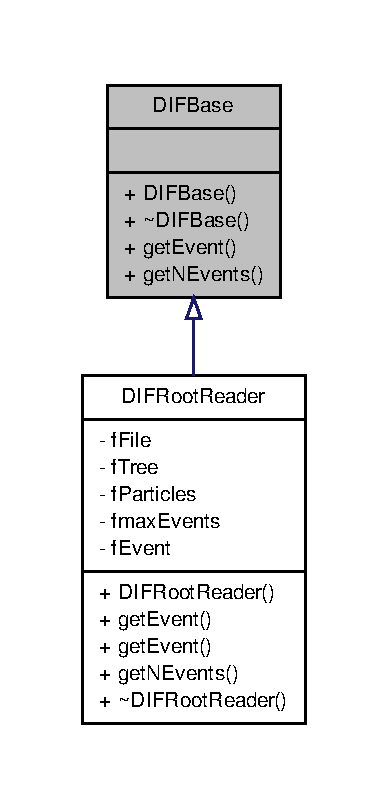
\includegraphics[width=186pt]{da/d1e/classDIFBase__inherit__graph}
\end{center}
\end{figure}
\subsection*{Public Member Functions}
\begin{DoxyCompactItemize}
\item 
\hyperlink{classDIFBase_acbbc1c92aa68251a8bc21a49d3c23374}{DIFBase} ()
\item 
virtual \hyperlink{classDIFBase_a36a102f92fd77b49a88274b88d150905}{$\sim$DIFBase} ()
\item 
virtual const int \hyperlink{classDIFBase_ab31cfae817f0420fa6a7b8b2cc013baa}{getEvent} (const int, \hyperlink{classPWAEvent}{PWAEvent} \&)=0
\item 
virtual const unsigned int \hyperlink{classDIFBase_a69e359ba0221a1b7bb32cdcbb819d56a}{getNEvents} () const =0
\end{DoxyCompactItemize}


\subsection{Detailed Description}
Data Interface Base-\/Class. 

\subsection{Constructor \& Destructor Documentation}
\hypertarget{classDIFBase_acbbc1c92aa68251a8bc21a49d3c23374}{
\index{DIFBase@{DIFBase}!DIFBase@{DIFBase}}
\index{DIFBase@{DIFBase}!DIFBase@{DIFBase}}
\subsubsection[{DIFBase}]{\setlength{\rightskip}{0pt plus 5cm}DIFBase::DIFBase (
\begin{DoxyParamCaption}
{}
\end{DoxyParamCaption}
)\hspace{0.3cm}{\ttfamily  \mbox{[}inline\mbox{]}}}}
\label{d9/db5/classDIFBase_acbbc1c92aa68251a8bc21a49d3c23374}
\hypertarget{classDIFBase_a36a102f92fd77b49a88274b88d150905}{
\index{DIFBase@{DIFBase}!$\sim$DIFBase@{$\sim$DIFBase}}
\index{$\sim$DIFBase@{$\sim$DIFBase}!DIFBase@{DIFBase}}
\subsubsection[{$\sim$DIFBase}]{\setlength{\rightskip}{0pt plus 5cm}virtual DIFBase::$\sim$DIFBase (
\begin{DoxyParamCaption}
{}
\end{DoxyParamCaption}
)\hspace{0.3cm}{\ttfamily  \mbox{[}inline, virtual\mbox{]}}}}
\label{d9/db5/classDIFBase_a36a102f92fd77b49a88274b88d150905}


\subsection{Member Function Documentation}
\hypertarget{classDIFBase_ab31cfae817f0420fa6a7b8b2cc013baa}{
\index{DIFBase@{DIFBase}!getEvent@{getEvent}}
\index{getEvent@{getEvent}!DIFBase@{DIFBase}}
\subsubsection[{getEvent}]{\setlength{\rightskip}{0pt plus 5cm}virtual const int DIFBase::getEvent (
\begin{DoxyParamCaption}
\item[{const int}]{, }
\item[{{\bf PWAEvent} \&}]{}
\end{DoxyParamCaption}
)\hspace{0.3cm}{\ttfamily  \mbox{[}pure virtual\mbox{]}}}}
\label{d9/db5/classDIFBase_ab31cfae817f0420fa6a7b8b2cc013baa}


Implemented in \hyperlink{classDIFRootReader_a2469dc5451328c7e802f2ff540842082}{DIFRootReader}.

\hypertarget{classDIFBase_a69e359ba0221a1b7bb32cdcbb819d56a}{
\index{DIFBase@{DIFBase}!getNEvents@{getNEvents}}
\index{getNEvents@{getNEvents}!DIFBase@{DIFBase}}
\subsubsection[{getNEvents}]{\setlength{\rightskip}{0pt plus 5cm}virtual const unsigned int DIFBase::getNEvents (
\begin{DoxyParamCaption}
{}
\end{DoxyParamCaption}
) const\hspace{0.3cm}{\ttfamily  \mbox{[}pure virtual\mbox{]}}}}
\label{d9/db5/classDIFBase_a69e359ba0221a1b7bb32cdcbb819d56a}


Implemented in \hyperlink{classDIFRootReader_a2cee7a677795a26ecef7cdf3129162ab}{DIFRootReader}.



The documentation for this class was generated from the following file:\begin{DoxyCompactItemize}
\item 
Core/\hyperlink{DIFBase_8hpp}{DIFBase.hpp}\end{DoxyCompactItemize}

\hypertarget{classDIFRootReader}{
\section{DIFRootReader Class Reference}
\label{dc/ddc/classDIFRootReader}\index{DIFRootReader@{DIFRootReader}}
}


Reader for data in Root-\/files.  




{\ttfamily \#include $<$DIFRootReader.hpp$>$}

Inheritance diagram for DIFRootReader:\begin{figure}[H]
\begin{center}
\leavevmode
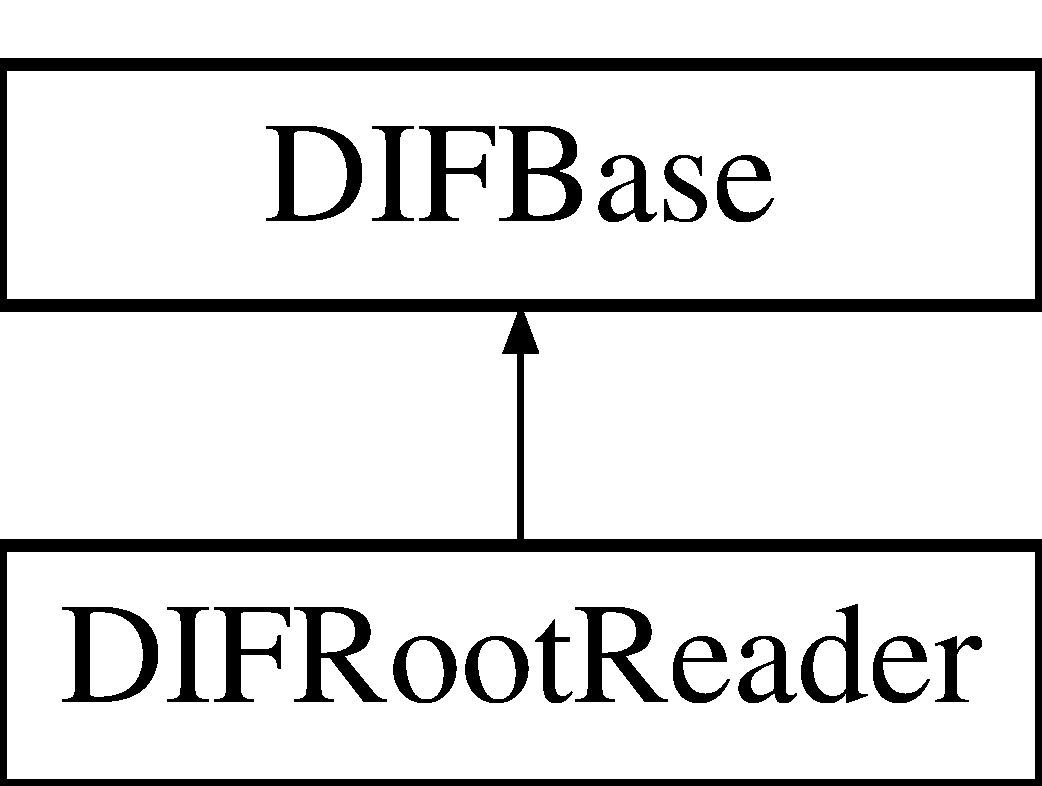
\includegraphics[height=2.000000cm]{dc/ddc/classDIFRootReader}
\end{center}
\end{figure}
\subsection*{Public Member Functions}
\begin{DoxyCompactItemize}
\item 
\hyperlink{classDIFRootReader_a627b25e9eba44a8485b445916f955333}{DIFRootReader} (string inConfigFile)
\begin{DoxyCompactList}\small\item\em Default Constructor (0x0) \end{DoxyCompactList}\item 
virtual const int \hyperlink{classDIFRootReader_a2469dc5451328c7e802f2ff540842082}{getEvent} (const int, \hyperlink{classPWAEvent}{PWAEvent} \&)
\item 
virtual const int \hyperlink{classDIFRootReader_a4d39cf2617a549c0fd6b097be8890756}{getEvent} (const int, TLorentzVector \&, TLorentzVector \&, double \&)
\item 
virtual const unsigned int \hyperlink{classDIFRootReader_a2cee7a677795a26ecef7cdf3129162ab}{getNEvents} () const 
\item 
virtual \hyperlink{classDIFRootReader_a3b2d897442630d757da57a3f2a83f7f3}{$\sim$DIFRootReader} ()
\end{DoxyCompactItemize}
\subsection*{Private Attributes}
\begin{DoxyCompactItemize}
\item 
TFile $\ast$ \hyperlink{classDIFRootReader_aad2ead3ab401eca6ec51939dfcfb923f}{fFile}
\item 
TTree $\ast$ \hyperlink{classDIFRootReader_a95ae7f9154ea46dbe4d2423e9d8f3c7d}{fTree}
\item 
TClonesArray $\ast$ \hyperlink{classDIFRootReader_a250796ef6bbe231cf75da5e985961ac1}{fParticles}
\item 
unsigned int \hyperlink{classDIFRootReader_a935660214d9cd8b2035471b7bccb2b1e}{fmaxEvents}
\item 
unsigned int \hyperlink{classDIFRootReader_aa4beae1437759d5d4fb7d3f357118fe8}{fEvent}
\end{DoxyCompactItemize}


\subsection{Detailed Description}
Reader for data in Root-\/files. 

\subsection{Constructor \& Destructor Documentation}
\hypertarget{classDIFRootReader_a627b25e9eba44a8485b445916f955333}{
\index{DIFRootReader@{DIFRootReader}!DIFRootReader@{DIFRootReader}}
\index{DIFRootReader@{DIFRootReader}!DIFRootReader@{DIFRootReader}}
\subsubsection[{DIFRootReader}]{\setlength{\rightskip}{0pt plus 5cm}DIFRootReader::DIFRootReader (
\begin{DoxyParamCaption}
\item[{string}]{inConfigFile}
\end{DoxyParamCaption}
)}}
\label{dc/ddc/classDIFRootReader_a627b25e9eba44a8485b445916f955333}


Default Constructor (0x0) 

\hypertarget{classDIFRootReader_a3b2d897442630d757da57a3f2a83f7f3}{
\index{DIFRootReader@{DIFRootReader}!$\sim$DIFRootReader@{$\sim$DIFRootReader}}
\index{$\sim$DIFRootReader@{$\sim$DIFRootReader}!DIFRootReader@{DIFRootReader}}
\subsubsection[{$\sim$DIFRootReader}]{\setlength{\rightskip}{0pt plus 5cm}DIFRootReader::$\sim$DIFRootReader (
\begin{DoxyParamCaption}
{}
\end{DoxyParamCaption}
)\hspace{0.3cm}{\ttfamily  \mbox{[}virtual\mbox{]}}}}
\label{dc/ddc/classDIFRootReader_a3b2d897442630d757da57a3f2a83f7f3}
Destructor 

\subsection{Member Function Documentation}
\hypertarget{classDIFRootReader_a2469dc5451328c7e802f2ff540842082}{
\index{DIFRootReader@{DIFRootReader}!getEvent@{getEvent}}
\index{getEvent@{getEvent}!DIFRootReader@{DIFRootReader}}
\subsubsection[{getEvent}]{\setlength{\rightskip}{0pt plus 5cm}const int DIFRootReader::getEvent (
\begin{DoxyParamCaption}
\item[{const int}]{i, }
\item[{{\bf PWAEvent} \&}]{inEvent}
\end{DoxyParamCaption}
)\hspace{0.3cm}{\ttfamily  \mbox{[}virtual\mbox{]}}}}
\label{dc/ddc/classDIFRootReader_a2469dc5451328c7e802f2ff540842082}


Implements \hyperlink{classDIFBase_ab31cfae817f0420fa6a7b8b2cc013baa}{DIFBase}.

\hypertarget{classDIFRootReader_a4d39cf2617a549c0fd6b097be8890756}{
\index{DIFRootReader@{DIFRootReader}!getEvent@{getEvent}}
\index{getEvent@{getEvent}!DIFRootReader@{DIFRootReader}}
\subsubsection[{getEvent}]{\setlength{\rightskip}{0pt plus 5cm}const int DIFRootReader::getEvent (
\begin{DoxyParamCaption}
\item[{const int}]{i, }
\item[{TLorentzVector \&}]{in1, }
\item[{TLorentzVector \&}]{in2, }
\item[{double \&}]{inm12}
\end{DoxyParamCaption}
)\hspace{0.3cm}{\ttfamily  \mbox{[}virtual\mbox{]}}}}
\label{dc/ddc/classDIFRootReader_a4d39cf2617a549c0fd6b097be8890756}
\hypertarget{classDIFRootReader_a2cee7a677795a26ecef7cdf3129162ab}{
\index{DIFRootReader@{DIFRootReader}!getNEvents@{getNEvents}}
\index{getNEvents@{getNEvents}!DIFRootReader@{DIFRootReader}}
\subsubsection[{getNEvents}]{\setlength{\rightskip}{0pt plus 5cm}virtual const unsigned int DIFRootReader::getNEvents (
\begin{DoxyParamCaption}
{}
\end{DoxyParamCaption}
) const\hspace{0.3cm}{\ttfamily  \mbox{[}inline, virtual\mbox{]}}}}
\label{dc/ddc/classDIFRootReader_a2cee7a677795a26ecef7cdf3129162ab}


Implements \hyperlink{classDIFBase_a69e359ba0221a1b7bb32cdcbb819d56a}{DIFBase}.



\subsection{Member Data Documentation}
\hypertarget{classDIFRootReader_aa4beae1437759d5d4fb7d3f357118fe8}{
\index{DIFRootReader@{DIFRootReader}!fEvent@{fEvent}}
\index{fEvent@{fEvent}!DIFRootReader@{DIFRootReader}}
\subsubsection[{fEvent}]{\setlength{\rightskip}{0pt plus 5cm}unsigned int {\bf DIFRootReader::fEvent}\hspace{0.3cm}{\ttfamily  \mbox{[}private\mbox{]}}}}
\label{dc/ddc/classDIFRootReader_aa4beae1437759d5d4fb7d3f357118fe8}
\hypertarget{classDIFRootReader_aad2ead3ab401eca6ec51939dfcfb923f}{
\index{DIFRootReader@{DIFRootReader}!fFile@{fFile}}
\index{fFile@{fFile}!DIFRootReader@{DIFRootReader}}
\subsubsection[{fFile}]{\setlength{\rightskip}{0pt plus 5cm}TFile$\ast$ {\bf DIFRootReader::fFile}\hspace{0.3cm}{\ttfamily  \mbox{[}private\mbox{]}}}}
\label{dc/ddc/classDIFRootReader_aad2ead3ab401eca6ec51939dfcfb923f}
\hypertarget{classDIFRootReader_a935660214d9cd8b2035471b7bccb2b1e}{
\index{DIFRootReader@{DIFRootReader}!fmaxEvents@{fmaxEvents}}
\index{fmaxEvents@{fmaxEvents}!DIFRootReader@{DIFRootReader}}
\subsubsection[{fmaxEvents}]{\setlength{\rightskip}{0pt plus 5cm}unsigned int {\bf DIFRootReader::fmaxEvents}\hspace{0.3cm}{\ttfamily  \mbox{[}private\mbox{]}}}}
\label{dc/ddc/classDIFRootReader_a935660214d9cd8b2035471b7bccb2b1e}
\hypertarget{classDIFRootReader_a250796ef6bbe231cf75da5e985961ac1}{
\index{DIFRootReader@{DIFRootReader}!fParticles@{fParticles}}
\index{fParticles@{fParticles}!DIFRootReader@{DIFRootReader}}
\subsubsection[{fParticles}]{\setlength{\rightskip}{0pt plus 5cm}TClonesArray$\ast$ {\bf DIFRootReader::fParticles}\hspace{0.3cm}{\ttfamily  \mbox{[}private\mbox{]}}}}
\label{dc/ddc/classDIFRootReader_a250796ef6bbe231cf75da5e985961ac1}
\hypertarget{classDIFRootReader_a95ae7f9154ea46dbe4d2423e9d8f3c7d}{
\index{DIFRootReader@{DIFRootReader}!fTree@{fTree}}
\index{fTree@{fTree}!DIFRootReader@{DIFRootReader}}
\subsubsection[{fTree}]{\setlength{\rightskip}{0pt plus 5cm}TTree$\ast$ {\bf DIFRootReader::fTree}\hspace{0.3cm}{\ttfamily  \mbox{[}private\mbox{]}}}}
\label{dc/ddc/classDIFRootReader_a95ae7f9154ea46dbe4d2423e9d8f3c7d}


The documentation for this class was generated from the following files:\begin{DoxyCompactItemize}
\item 
DIFRoot2Part/\hyperlink{DIFRootReader_8hpp}{DIFRootReader.hpp}\item 
DIFRoot2Part/\hyperlink{DIFRootReader_8cpp}{DIFRootReader.cpp}\end{DoxyCompactItemize}

\hypertarget{classEIFBase}{
\section{EIFBase Class Reference}
\label{df/d13/classEIFBase}\index{EIFBase@{EIFBase}}
}


Estimator Interface Base-\/Class.  




{\ttfamily \#include $<$EIFBase.hpp$>$}



Inheritance diagram for EIFBase:\nopagebreak
\begin{figure}[H]
\begin{center}
\leavevmode
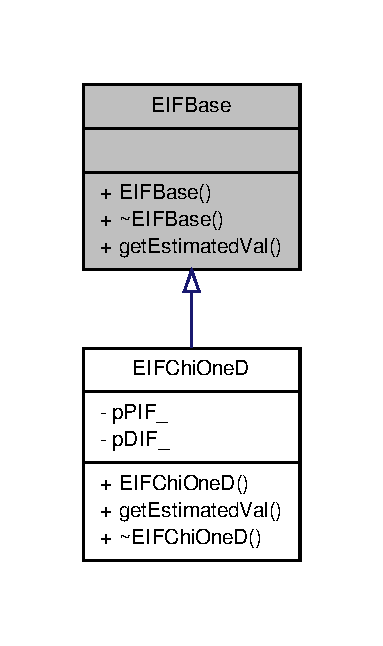
\includegraphics[width=186pt]{d7/d7a/classEIFBase__inherit__graph}
\end{center}
\end{figure}


Collaboration diagram for EIFBase:\nopagebreak
\begin{figure}[H]
\begin{center}
\leavevmode
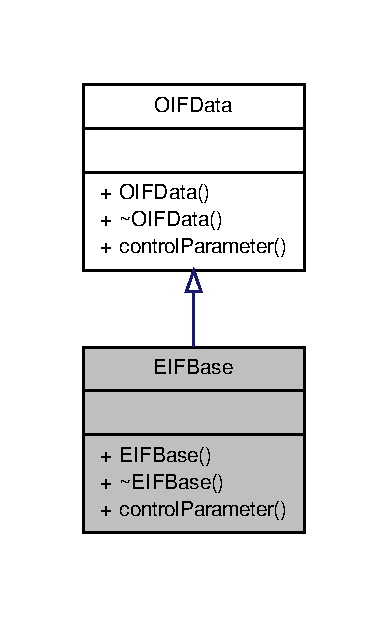
\includegraphics[width=186pt]{db/da5/classEIFBase__coll__graph}
\end{center}
\end{figure}
\subsection*{Public Member Functions}
\begin{DoxyCompactItemize}
\item 
\hyperlink{classEIFBase_a8b6ea6ef6b90d40293b55a71249cb5f0}{EIFBase} ()
\item 
virtual \hyperlink{classEIFBase_ae4253811072d1d4251a009bda238f450}{$\sim$EIFBase} ()
\item 
virtual double \hyperlink{classEIFBase_a85937003fd68b507ddc99bfcee3a4b27}{controlParameter} (const std::vector$<$ \hyperlink{classPWAParameter}{PWAParameter}$<$ double $>$ $>$ \&minPar)=0
\end{DoxyCompactItemize}


\subsection{Detailed Description}
Estimator Interface Base-\/Class. 

\subsection{Constructor \& Destructor Documentation}
\hypertarget{classEIFBase_a8b6ea6ef6b90d40293b55a71249cb5f0}{
\index{EIFBase@{EIFBase}!EIFBase@{EIFBase}}
\index{EIFBase@{EIFBase}!EIFBase@{EIFBase}}
\subsubsection[{EIFBase}]{\setlength{\rightskip}{0pt plus 5cm}EIFBase::EIFBase (
\begin{DoxyParamCaption}
{}
\end{DoxyParamCaption}
)\hspace{0.3cm}{\ttfamily  \mbox{[}inline\mbox{]}}}}
\label{df/d13/classEIFBase_a8b6ea6ef6b90d40293b55a71249cb5f0}
\hypertarget{classEIFBase_ae4253811072d1d4251a009bda238f450}{
\index{EIFBase@{EIFBase}!$\sim$EIFBase@{$\sim$EIFBase}}
\index{$\sim$EIFBase@{$\sim$EIFBase}!EIFBase@{EIFBase}}
\subsubsection[{$\sim$EIFBase}]{\setlength{\rightskip}{0pt plus 5cm}virtual EIFBase::$\sim$EIFBase (
\begin{DoxyParamCaption}
{}
\end{DoxyParamCaption}
)\hspace{0.3cm}{\ttfamily  \mbox{[}inline, virtual\mbox{]}}}}
\label{df/d13/classEIFBase_ae4253811072d1d4251a009bda238f450}


\subsection{Member Function Documentation}
\hypertarget{classEIFBase_a85937003fd68b507ddc99bfcee3a4b27}{
\index{EIFBase@{EIFBase}!controlParameter@{controlParameter}}
\index{controlParameter@{controlParameter}!EIFBase@{EIFBase}}
\subsubsection[{controlParameter}]{\setlength{\rightskip}{0pt plus 5cm}virtual double EIFBase::controlParameter (
\begin{DoxyParamCaption}
\item[{const std::vector$<$ {\bf PWAParameter}$<$ double $>$ $>$ \&}]{minPar}
\end{DoxyParamCaption}
)\hspace{0.3cm}{\ttfamily  \mbox{[}pure virtual\mbox{]}}}}
\label{df/d13/classEIFBase_a85937003fd68b507ddc99bfcee3a4b27}


Implements \hyperlink{classOIFData_a12eef51d074a73b5b261c411e79cbb37}{OIFData}.



Implemented in \hyperlink{classEIFChiOneD_a014a763220034f5547c2d395b3508b8d}{EIFChiOneD}.



The documentation for this class was generated from the following file:\begin{DoxyCompactItemize}
\item 
Core/\hyperlink{EIFBase_8hpp}{EIFBase.hpp}\end{DoxyCompactItemize}

\hypertarget{classEIFChiOneD}{
\section{EIFChiOneD Class Reference}
\label{db/d1d/classEIFChiOneD}\index{EIFChiOneD@{EIFChiOneD}}
}


Simple $\chi^{2}$-\/Estimator.  




{\ttfamily \#include $<$EIFChiOneD.hpp$>$}



Inheritance diagram for EIFChiOneD:\nopagebreak
\begin{figure}[H]
\begin{center}
\leavevmode
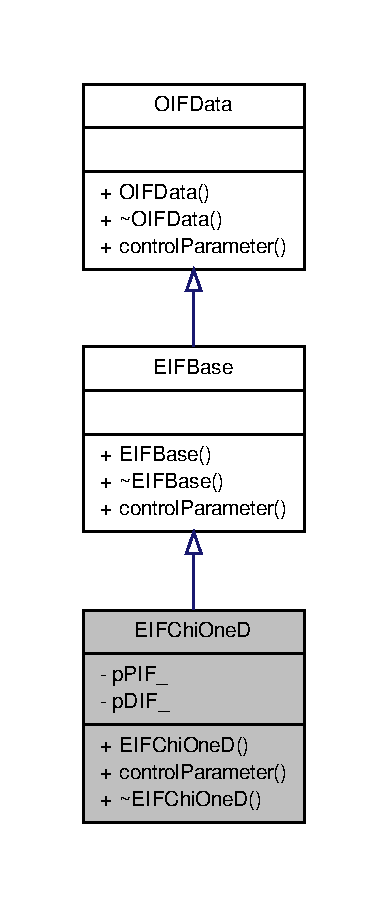
\includegraphics[width=186pt]{dc/de7/classEIFChiOneD__inherit__graph}
\end{center}
\end{figure}


Collaboration diagram for EIFChiOneD:\nopagebreak
\begin{figure}[H]
\begin{center}
\leavevmode
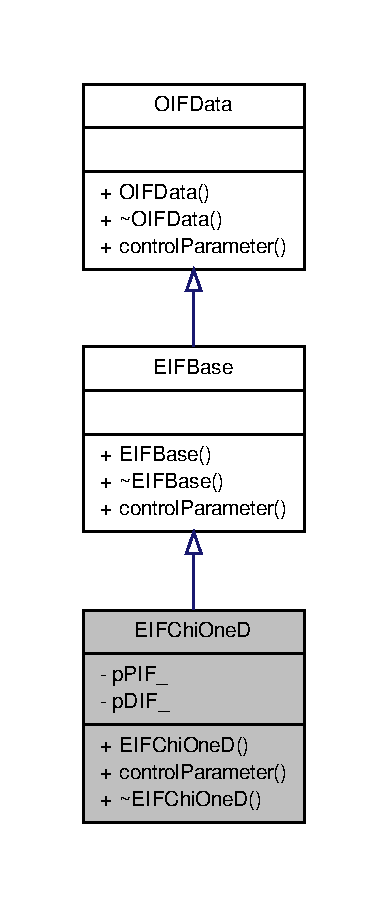
\includegraphics[width=186pt]{d2/db1/classEIFChiOneD__coll__graph}
\end{center}
\end{figure}
\subsection*{Public Member Functions}
\begin{DoxyCompactItemize}
\item 
\hyperlink{classEIFChiOneD_a777b712b06dd2c760f1071e2cc932eba}{EIFChiOneD} (std::shared\_\-ptr$<$ \hyperlink{classPIFBase}{PIFBase} $>$, std::shared\_\-ptr$<$ \hyperlink{classDIFBase}{DIFBase} $>$)
\begin{DoxyCompactList}\small\item\em Default Constructor (0x0) \end{DoxyCompactList}\item 
virtual double \hyperlink{classEIFChiOneD_a014a763220034f5547c2d395b3508b8d}{controlParameter} (const std::vector$<$ \hyperlink{classPWAParameter}{PWAParameter}$<$ double $>$ $>$ \&minPar)
\item 
virtual \hyperlink{classEIFChiOneD_ac826a3c3af84dd72fd96e32d597dd560}{$\sim$EIFChiOneD} ()
\end{DoxyCompactItemize}
\subsection*{Private Attributes}
\begin{DoxyCompactItemize}
\item 
std::shared\_\-ptr$<$ \hyperlink{classPIFBase}{PIFBase} $>$ \hyperlink{classEIFChiOneD_a54b481cfd837c78597ef9a7d7a872961}{pPIF\_\-}
\item 
std::shared\_\-ptr$<$ \hyperlink{classDIFBase}{DIFBase} $>$ \hyperlink{classEIFChiOneD_a2700a77eb9736ea1468adea10acdd823}{pDIF\_\-}
\end{DoxyCompactItemize}


\subsection{Detailed Description}
Simple $\chi^{2}$-\/Estimator. 

\subsection{Constructor \& Destructor Documentation}
\hypertarget{classEIFChiOneD_a777b712b06dd2c760f1071e2cc932eba}{
\index{EIFChiOneD@{EIFChiOneD}!EIFChiOneD@{EIFChiOneD}}
\index{EIFChiOneD@{EIFChiOneD}!EIFChiOneD@{EIFChiOneD}}
\subsubsection[{EIFChiOneD}]{\setlength{\rightskip}{0pt plus 5cm}EIFChiOneD::EIFChiOneD (
\begin{DoxyParamCaption}
\item[{std::shared\_\-ptr$<$ {\bf PIFBase} $>$}]{inPIF, }
\item[{std::shared\_\-ptr$<$ {\bf DIFBase} $>$}]{inDIF}
\end{DoxyParamCaption}
)}}
\label{db/d1d/classEIFChiOneD_a777b712b06dd2c760f1071e2cc932eba}


Default Constructor (0x0) 

\hypertarget{classEIFChiOneD_ac826a3c3af84dd72fd96e32d597dd560}{
\index{EIFChiOneD@{EIFChiOneD}!$\sim$EIFChiOneD@{$\sim$EIFChiOneD}}
\index{$\sim$EIFChiOneD@{$\sim$EIFChiOneD}!EIFChiOneD@{EIFChiOneD}}
\subsubsection[{$\sim$EIFChiOneD}]{\setlength{\rightskip}{0pt plus 5cm}EIFChiOneD::$\sim$EIFChiOneD (
\begin{DoxyParamCaption}
{}
\end{DoxyParamCaption}
)\hspace{0.3cm}{\ttfamily  \mbox{[}virtual\mbox{]}}}}
\label{db/d1d/classEIFChiOneD_ac826a3c3af84dd72fd96e32d597dd560}
Destructor 

\subsection{Member Function Documentation}
\hypertarget{classEIFChiOneD_a014a763220034f5547c2d395b3508b8d}{
\index{EIFChiOneD@{EIFChiOneD}!controlParameter@{controlParameter}}
\index{controlParameter@{controlParameter}!EIFChiOneD@{EIFChiOneD}}
\subsubsection[{controlParameter}]{\setlength{\rightskip}{0pt plus 5cm}double EIFChiOneD::controlParameter (
\begin{DoxyParamCaption}
\item[{const std::vector$<$ {\bf PWAParameter}$<$ double $>$ $>$ \&}]{minPar}
\end{DoxyParamCaption}
)\hspace{0.3cm}{\ttfamily  \mbox{[}virtual\mbox{]}}}}
\label{db/d1d/classEIFChiOneD_a014a763220034f5547c2d395b3508b8d}


Implements \hyperlink{classEIFBase_a85937003fd68b507ddc99bfcee3a4b27}{EIFBase}.



\subsection{Member Data Documentation}
\hypertarget{classEIFChiOneD_a2700a77eb9736ea1468adea10acdd823}{
\index{EIFChiOneD@{EIFChiOneD}!pDIF\_\-@{pDIF\_\-}}
\index{pDIF\_\-@{pDIF\_\-}!EIFChiOneD@{EIFChiOneD}}
\subsubsection[{pDIF\_\-}]{\setlength{\rightskip}{0pt plus 5cm}std::shared\_\-ptr$<${\bf DIFBase}$>$ {\bf EIFChiOneD::pDIF\_\-}\hspace{0.3cm}{\ttfamily  \mbox{[}private\mbox{]}}}}
\label{db/d1d/classEIFChiOneD_a2700a77eb9736ea1468adea10acdd823}
\hypertarget{classEIFChiOneD_a54b481cfd837c78597ef9a7d7a872961}{
\index{EIFChiOneD@{EIFChiOneD}!pPIF\_\-@{pPIF\_\-}}
\index{pPIF\_\-@{pPIF\_\-}!EIFChiOneD@{EIFChiOneD}}
\subsubsection[{pPIF\_\-}]{\setlength{\rightskip}{0pt plus 5cm}std::shared\_\-ptr$<${\bf PIFBase}$>$ {\bf EIFChiOneD::pPIF\_\-}\hspace{0.3cm}{\ttfamily  \mbox{[}private\mbox{]}}}}
\label{db/d1d/classEIFChiOneD_a54b481cfd837c78597ef9a7d7a872961}


The documentation for this class was generated from the following files:\begin{DoxyCompactItemize}
\item 
EIFChiOneD/\hyperlink{EIFChiOneD_8hpp}{EIFChiOneD.hpp}\item 
EIFChiOneD/\hyperlink{EIFChiOneD_8cpp}{EIFChiOneD.cpp}\end{DoxyCompactItemize}

\hypertarget{classGArgumentParser}{
\section{GArgumentParser Class Reference}
\label{d0/d39/classGArgumentParser}\index{GArgumentParser@{GArgumentParser}}
}


Geneva Argument Parser.  




{\ttfamily \#include $<$GArgumentParser.hpp$>$}



\subsection{Detailed Description}
Geneva Argument Parser. 

The documentation for this class was generated from the following file:\begin{DoxyCompactItemize}
\item 
OIFGeneva/\hyperlink{GArgumentParser_8hpp}{GArgumentParser.hpp}\end{DoxyCompactItemize}

\hypertarget{classGem_1_1Geneva_1_1GStartIndividual}{
\section{Gem::Geneva::GStartIndividual Class Reference}
\label{dd/d14/classGem_1_1Geneva_1_1GStartIndividual}\index{Gem::Geneva::GStartIndividual@{Gem::Geneva::GStartIndividual}}
}


{\ttfamily \#include $<$GStartIndividual.hpp$>$}

\subsection*{Public Member Functions}
\begin{DoxyCompactItemize}
\item 
\hyperlink{classGem_1_1Geneva_1_1GStartIndividual_af12cc2d6bd870fa2574ef52a3f6a5802}{GStartIndividual} (std::shared\_\-ptr$<$ \hyperlink{classOIFData}{OIFData} $>$ data, unsigned int parDim, double $\ast$val, double $\ast$min, double $\ast$max, double $\ast$err)
\item 
\hyperlink{classGem_1_1Geneva_1_1GStartIndividual_ac6e59c84c2f7aa4400234906f7f1409a}{GStartIndividual} (const \hyperlink{classGem_1_1Geneva_1_1GStartIndividual}{GStartIndividual} \&cp)
\item 
virtual \hyperlink{classGem_1_1Geneva_1_1GStartIndividual_ac39a07f9e9829da80f9eae7277ee5982}{$\sim$GStartIndividual} ()
\item 
bool \hyperlink{classGem_1_1Geneva_1_1GStartIndividual_a038ae274cb482688e6f81c158f1f1726}{getPar} (std::vector$<$ \hyperlink{classPWAParameter}{PWAParameter}$<$ double $>$ $>$ \&val)
\item 
const \hyperlink{classGem_1_1Geneva_1_1GStartIndividual}{GStartIndividual} \& \hyperlink{classGem_1_1Geneva_1_1GStartIndividual_ac490d0618fbf311eb90768fc090c63aa}{operator=} (const \hyperlink{classGem_1_1Geneva_1_1GStartIndividual}{GStartIndividual} \&cp)
\item 
bool \hyperlink{classGem_1_1Geneva_1_1GStartIndividual_a24c9a1156f06dad45afb2fc52d73ca47}{operator==} (const \hyperlink{classGem_1_1Geneva_1_1GStartIndividual}{GStartIndividual} \&cp) const 
\item 
bool \hyperlink{classGem_1_1Geneva_1_1GStartIndividual_abf9e54ba75293a2cf4d9cc8ca7716f63}{operator!=} (const \hyperlink{classGem_1_1Geneva_1_1GStartIndividual}{GStartIndividual} \&cp) const 
\item 
boost::optional$<$ std::string $>$ \hyperlink{classGem_1_1Geneva_1_1GStartIndividual_af821f39180d83fcb61b7cd49a2679a4f}{checkRelationshipWith} (const GObject \&cp, const Gem::Common::expectation \&e, const double \&limit, const std::string \&caller, const std::string \&y\_\-name, const bool \&withMessages) const 
\end{DoxyCompactItemize}
\subsection*{Protected Member Functions}
\begin{DoxyCompactItemize}
\item 
virtual void \hyperlink{classGem_1_1Geneva_1_1GStartIndividual_a722b0e83493f9e06e1facca0f2909667}{load\_\-} (const GObject $\ast$cp)
\item 
virtual GObject $\ast$ \hyperlink{classGem_1_1Geneva_1_1GStartIndividual_a089f4f854c65668d4af94062d494ec34}{clone\_\-} () const 
\item 
virtual double \hyperlink{classGem_1_1Geneva_1_1GStartIndividual_a0ca77799d18c829f22538c1ba08c0242}{fitnessCalculation} ()
\end{DoxyCompactItemize}
\subsection*{Private Member Functions}
\begin{DoxyCompactItemize}
\item 
{\footnotesize template$<$typename Archive $>$ }\\void \hyperlink{classGem_1_1Geneva_1_1GStartIndividual_a9259159c50c1e5084120947e0598bda3}{serialize} (Archive \&ar, const unsigned int)
\item 
\hyperlink{classGem_1_1Geneva_1_1GStartIndividual_a8942d3c6bfa0399fdfcd8025e03107fb}{GStartIndividual} ()
\end{DoxyCompactItemize}
\subsection*{Private Attributes}
\begin{DoxyCompactItemize}
\item 
std::shared\_\-ptr$<$ \hyperlink{classOIFData}{OIFData} $>$ \hyperlink{classGem_1_1Geneva_1_1GStartIndividual_a38407e1c34927cd8675f7f289d20bead}{theData}
\end{DoxyCompactItemize}
\subsection*{Friends}
\begin{DoxyCompactItemize}
\item 
class \hyperlink{classGem_1_1Geneva_1_1GStartIndividual_ac98d07dd8f7b70e16ccb9a01abf56b9c}{boost::serialization::access}
\end{DoxyCompactItemize}


\subsection{Detailed Description}
This individual searches for the minimum of a parabola of a given dimension, It is part of a complete example that lets users adapt their optimization problems more easily to the \hyperlink{namespaceGem_1_1Geneva}{Geneva} conventions. 

\subsection{Constructor \& Destructor Documentation}
\hypertarget{classGem_1_1Geneva_1_1GStartIndividual_af12cc2d6bd870fa2574ef52a3f6a5802}{
\index{Gem::Geneva::GStartIndividual@{Gem::Geneva::GStartIndividual}!GStartIndividual@{GStartIndividual}}
\index{GStartIndividual@{GStartIndividual}!Gem::Geneva::GStartIndividual@{Gem::Geneva::GStartIndividual}}
\subsubsection[{GStartIndividual}]{\setlength{\rightskip}{0pt plus 5cm}Gem::Geneva::GStartIndividual::GStartIndividual (
\begin{DoxyParamCaption}
\item[{std::shared\_\-ptr$<$ {\bf OIFData} $>$}]{data, }
\item[{unsigned int}]{parDim, }
\item[{double $\ast$}]{val, }
\item[{double $\ast$}]{min, }
\item[{double $\ast$}]{max, }
\item[{double $\ast$}]{err}
\end{DoxyParamCaption}
)\hspace{0.3cm}{\ttfamily  \mbox{[}inline\mbox{]}}}}
\label{dd/d14/classGem_1_1Geneva_1_1GStartIndividual_af12cc2d6bd870fa2574ef52a3f6a5802}
A simple constructor that initializes this object with a collection of bounded double variables.


\begin{DoxyParams}{Parameters}
{\em data} & The data to be optimized to \\
\hline
{\em parDim} & The amount of variables \\
\hline
{\em val} & The value of the variables \\
\hline
{\em min} & The lower boundary of the variables \\
\hline
{\em max} & The upper boundary of the variables \\
\hline
{\em err} & The error of the variables \\
\hline
\end{DoxyParams}
\hypertarget{classGem_1_1Geneva_1_1GStartIndividual_ac6e59c84c2f7aa4400234906f7f1409a}{
\index{Gem::Geneva::GStartIndividual@{Gem::Geneva::GStartIndividual}!GStartIndividual@{GStartIndividual}}
\index{GStartIndividual@{GStartIndividual}!Gem::Geneva::GStartIndividual@{Gem::Geneva::GStartIndividual}}
\subsubsection[{GStartIndividual}]{\setlength{\rightskip}{0pt plus 5cm}Gem::Geneva::GStartIndividual::GStartIndividual (
\begin{DoxyParamCaption}
\item[{const {\bf GStartIndividual} \&}]{cp}
\end{DoxyParamCaption}
)\hspace{0.3cm}{\ttfamily  \mbox{[}inline\mbox{]}}}}
\label{dd/d14/classGem_1_1Geneva_1_1GStartIndividual_ac6e59c84c2f7aa4400234906f7f1409a}
A standard copy constructor


\begin{DoxyParams}{Parameters}
{\em cp} & A copy of another \hyperlink{classGem_1_1Geneva_1_1GStartIndividual}{GStartIndividual} \\
\hline
\end{DoxyParams}
\hypertarget{classGem_1_1Geneva_1_1GStartIndividual_ac39a07f9e9829da80f9eae7277ee5982}{
\index{Gem::Geneva::GStartIndividual@{Gem::Geneva::GStartIndividual}!$\sim$GStartIndividual@{$\sim$GStartIndividual}}
\index{$\sim$GStartIndividual@{$\sim$GStartIndividual}!Gem::Geneva::GStartIndividual@{Gem::Geneva::GStartIndividual}}
\subsubsection[{$\sim$GStartIndividual}]{\setlength{\rightskip}{0pt plus 5cm}virtual Gem::Geneva::GStartIndividual::$\sim$GStartIndividual (
\begin{DoxyParamCaption}
{}
\end{DoxyParamCaption}
)\hspace{0.3cm}{\ttfamily  \mbox{[}inline, virtual\mbox{]}}}}
\label{dd/d14/classGem_1_1Geneva_1_1GStartIndividual_ac39a07f9e9829da80f9eae7277ee5982}
The standard destructor \hypertarget{classGem_1_1Geneva_1_1GStartIndividual_a8942d3c6bfa0399fdfcd8025e03107fb}{
\index{Gem::Geneva::GStartIndividual@{Gem::Geneva::GStartIndividual}!GStartIndividual@{GStartIndividual}}
\index{GStartIndividual@{GStartIndividual}!Gem::Geneva::GStartIndividual@{Gem::Geneva::GStartIndividual}}
\subsubsection[{GStartIndividual}]{\setlength{\rightskip}{0pt plus 5cm}Gem::Geneva::GStartIndividual::GStartIndividual (
\begin{DoxyParamCaption}
{}
\end{DoxyParamCaption}
)\hspace{0.3cm}{\ttfamily  \mbox{[}inline, private\mbox{]}}}}
\label{dd/d14/classGem_1_1Geneva_1_1GStartIndividual_a8942d3c6bfa0399fdfcd8025e03107fb}
The default constructor. Intentionally private and empty, as it is only needed for serialization purposes. 

\subsection{Member Function Documentation}
\hypertarget{classGem_1_1Geneva_1_1GStartIndividual_af821f39180d83fcb61b7cd49a2679a4f}{
\index{Gem::Geneva::GStartIndividual@{Gem::Geneva::GStartIndividual}!checkRelationshipWith@{checkRelationshipWith}}
\index{checkRelationshipWith@{checkRelationshipWith}!Gem::Geneva::GStartIndividual@{Gem::Geneva::GStartIndividual}}
\subsubsection[{checkRelationshipWith}]{\setlength{\rightskip}{0pt plus 5cm}boost::optional$<$std::string$>$ Gem::Geneva::GStartIndividual::checkRelationshipWith (
\begin{DoxyParamCaption}
\item[{const GObject \&}]{cp, }
\item[{const Gem::Common::expectation \&}]{e, }
\item[{const double \&}]{limit, }
\item[{const std::string \&}]{caller, }
\item[{const std::string \&}]{y\_\-name, }
\item[{const bool \&}]{withMessages}
\end{DoxyParamCaption}
) const\hspace{0.3cm}{\ttfamily  \mbox{[}inline\mbox{]}}}}
\label{dd/d14/classGem_1_1Geneva_1_1GStartIndividual_af821f39180d83fcb61b7cd49a2679a4f}
Checks whether a given expectation for the relationship between this object and another object is fulfilled.

NOTE: THIS FUNCTION IS OPTIONAL AND IS MAINLY USED IN CONJUNCTION WITH UNIT TESTS. You do not need it if you do not intend to perform unit tests.


\begin{DoxyParams}{Parameters}
{\em cp} & A constant reference to another object, camouflaged as a GObject \\
\hline
{\em e} & The expected outcome of the comparison \\
\hline
{\em limit} & The maximum deviation for floating point values (important for similarity checks) \\
\hline
{\em caller} & An identifier for the calling entity \\
\hline
{\em y\_\-name} & An identifier for the object that should be compared to this one \\
\hline
{\em withMessages} & Whether or not information should be emitted in case of deviations from the expected outcome \\
\hline
\end{DoxyParams}
\begin{DoxyReturn}{Returns}
A boost::optional$<$std::string$>$ object that holds a descriptive string if expectations were not met 
\end{DoxyReturn}
\hypertarget{classGem_1_1Geneva_1_1GStartIndividual_a089f4f854c65668d4af94062d494ec34}{
\index{Gem::Geneva::GStartIndividual@{Gem::Geneva::GStartIndividual}!clone\_\-@{clone\_\-}}
\index{clone\_\-@{clone\_\-}!Gem::Geneva::GStartIndividual@{Gem::Geneva::GStartIndividual}}
\subsubsection[{clone\_\-}]{\setlength{\rightskip}{0pt plus 5cm}virtual GObject$\ast$ Gem::Geneva::GStartIndividual::clone\_\- (
\begin{DoxyParamCaption}
{}
\end{DoxyParamCaption}
) const\hspace{0.3cm}{\ttfamily  \mbox{[}inline, protected, virtual\mbox{]}}}}
\label{dd/d14/classGem_1_1Geneva_1_1GStartIndividual_a089f4f854c65668d4af94062d494ec34}
Creates a deep clone of this object

\begin{DoxyReturn}{Returns}
A deep clone of this object, camouflaged as a GObject 
\end{DoxyReturn}
\hypertarget{classGem_1_1Geneva_1_1GStartIndividual_a0ca77799d18c829f22538c1ba08c0242}{
\index{Gem::Geneva::GStartIndividual@{Gem::Geneva::GStartIndividual}!fitnessCalculation@{fitnessCalculation}}
\index{fitnessCalculation@{fitnessCalculation}!Gem::Geneva::GStartIndividual@{Gem::Geneva::GStartIndividual}}
\subsubsection[{fitnessCalculation}]{\setlength{\rightskip}{0pt plus 5cm}virtual double Gem::Geneva::GStartIndividual::fitnessCalculation (
\begin{DoxyParamCaption}
{}
\end{DoxyParamCaption}
)\hspace{0.3cm}{\ttfamily  \mbox{[}inline, protected, virtual\mbox{]}}}}
\label{dd/d14/classGem_1_1Geneva_1_1GStartIndividual_a0ca77799d18c829f22538c1ba08c0242}
The actual fitness calculation takes place here.

\begin{DoxyReturn}{Returns}
The value of this object 
\end{DoxyReturn}
\hypertarget{classGem_1_1Geneva_1_1GStartIndividual_a038ae274cb482688e6f81c158f1f1726}{
\index{Gem::Geneva::GStartIndividual@{Gem::Geneva::GStartIndividual}!getPar@{getPar}}
\index{getPar@{getPar}!Gem::Geneva::GStartIndividual@{Gem::Geneva::GStartIndividual}}
\subsubsection[{getPar}]{\setlength{\rightskip}{0pt plus 5cm}bool Gem::Geneva::GStartIndividual::getPar (
\begin{DoxyParamCaption}
\item[{std::vector$<$ {\bf PWAParameter}$<$ double $>$ $>$ \&}]{val}
\end{DoxyParamCaption}
)\hspace{0.3cm}{\ttfamily  \mbox{[}inline\mbox{]}}}}
\label{dd/d14/classGem_1_1Geneva_1_1GStartIndividual_a038ae274cb482688e6f81c158f1f1726}
\hypertarget{classGem_1_1Geneva_1_1GStartIndividual_a722b0e83493f9e06e1facca0f2909667}{
\index{Gem::Geneva::GStartIndividual@{Gem::Geneva::GStartIndividual}!load\_\-@{load\_\-}}
\index{load\_\-@{load\_\-}!Gem::Geneva::GStartIndividual@{Gem::Geneva::GStartIndividual}}
\subsubsection[{load\_\-}]{\setlength{\rightskip}{0pt plus 5cm}virtual void Gem::Geneva::GStartIndividual::load\_\- (
\begin{DoxyParamCaption}
\item[{const GObject $\ast$}]{cp}
\end{DoxyParamCaption}
)\hspace{0.3cm}{\ttfamily  \mbox{[}inline, protected, virtual\mbox{]}}}}
\label{dd/d14/classGem_1_1Geneva_1_1GStartIndividual_a722b0e83493f9e06e1facca0f2909667}
Loads the data of another \hyperlink{classGem_1_1Geneva_1_1GStartIndividual}{GStartIndividual}, camouflaged as a GObject.


\begin{DoxyParams}{Parameters}
{\em cp} & A copy of another \hyperlink{classGem_1_1Geneva_1_1GStartIndividual}{GStartIndividual}, camouflaged as a GObject \\
\hline
\end{DoxyParams}
\hypertarget{classGem_1_1Geneva_1_1GStartIndividual_abf9e54ba75293a2cf4d9cc8ca7716f63}{
\index{Gem::Geneva::GStartIndividual@{Gem::Geneva::GStartIndividual}!operator!=@{operator!=}}
\index{operator!=@{operator!=}!Gem::Geneva::GStartIndividual@{Gem::Geneva::GStartIndividual}}
\subsubsection[{operator!=}]{\setlength{\rightskip}{0pt plus 5cm}bool Gem::Geneva::GStartIndividual::operator!= (
\begin{DoxyParamCaption}
\item[{const {\bf GStartIndividual} \&}]{cp}
\end{DoxyParamCaption}
) const\hspace{0.3cm}{\ttfamily  \mbox{[}inline\mbox{]}}}}
\label{dd/d14/classGem_1_1Geneva_1_1GStartIndividual_abf9e54ba75293a2cf4d9cc8ca7716f63}
Checks for inequality with another \hyperlink{classGem_1_1Geneva_1_1GStartIndividual}{GStartIndividual} object.

NOTE: THIS FUNCTION IS OPTIONAL AND IS MAINLY USED IN CONJUNCTION WITH UNIT TESTS. You do not need it if you do not intend to perform unit tests.


\begin{DoxyParams}{Parameters}
{\em cp} & A constant reference to another \hyperlink{classGem_1_1Geneva_1_1GStartIndividual}{GStartIndividual} object \\
\hline
\end{DoxyParams}
\begin{DoxyReturn}{Returns}
A boolean indicating whether both objects are inequal 
\end{DoxyReturn}
\hypertarget{classGem_1_1Geneva_1_1GStartIndividual_ac490d0618fbf311eb90768fc090c63aa}{
\index{Gem::Geneva::GStartIndividual@{Gem::Geneva::GStartIndividual}!operator=@{operator=}}
\index{operator=@{operator=}!Gem::Geneva::GStartIndividual@{Gem::Geneva::GStartIndividual}}
\subsubsection[{operator=}]{\setlength{\rightskip}{0pt plus 5cm}const {\bf GStartIndividual}\& Gem::Geneva::GStartIndividual::operator= (
\begin{DoxyParamCaption}
\item[{const {\bf GStartIndividual} \&}]{cp}
\end{DoxyParamCaption}
)\hspace{0.3cm}{\ttfamily  \mbox{[}inline\mbox{]}}}}
\label{dd/d14/classGem_1_1Geneva_1_1GStartIndividual_ac490d0618fbf311eb90768fc090c63aa}
A standard assignment operator


\begin{DoxyParams}{Parameters}
{\em cp} & A copy of another \hyperlink{classGem_1_1Geneva_1_1GStartIndividual}{GStartIndividual} object \\
\hline
\end{DoxyParams}
\begin{DoxyReturn}{Returns}
A constant reference to this object 
\end{DoxyReturn}
\hypertarget{classGem_1_1Geneva_1_1GStartIndividual_a24c9a1156f06dad45afb2fc52d73ca47}{
\index{Gem::Geneva::GStartIndividual@{Gem::Geneva::GStartIndividual}!operator==@{operator==}}
\index{operator==@{operator==}!Gem::Geneva::GStartIndividual@{Gem::Geneva::GStartIndividual}}
\subsubsection[{operator==}]{\setlength{\rightskip}{0pt plus 5cm}bool Gem::Geneva::GStartIndividual::operator== (
\begin{DoxyParamCaption}
\item[{const {\bf GStartIndividual} \&}]{cp}
\end{DoxyParamCaption}
) const\hspace{0.3cm}{\ttfamily  \mbox{[}inline\mbox{]}}}}
\label{dd/d14/classGem_1_1Geneva_1_1GStartIndividual_a24c9a1156f06dad45afb2fc52d73ca47}
Checks for equality with another \hyperlink{classGem_1_1Geneva_1_1GStartIndividual}{GStartIndividual} object.

NOTE: THIS FUNCTION IS OPTIONAL AND IS MAINLY USED IN CONJUNCTION WITH UNIT TESTS. You do not need it if you do not intend to perform unit tests.


\begin{DoxyParams}{Parameters}
{\em cp} & A constant reference to another \hyperlink{classGem_1_1Geneva_1_1GStartIndividual}{GStartIndividual} object \\
\hline
\end{DoxyParams}
\begin{DoxyReturn}{Returns}
A boolean indicating whether both objects are equal 
\end{DoxyReturn}
\hypertarget{classGem_1_1Geneva_1_1GStartIndividual_a9259159c50c1e5084120947e0598bda3}{
\index{Gem::Geneva::GStartIndividual@{Gem::Geneva::GStartIndividual}!serialize@{serialize}}
\index{serialize@{serialize}!Gem::Geneva::GStartIndividual@{Gem::Geneva::GStartIndividual}}
\subsubsection[{serialize}]{\setlength{\rightskip}{0pt plus 5cm}template$<$typename Archive $>$ void Gem::Geneva::GStartIndividual::serialize (
\begin{DoxyParamCaption}
\item[{Archive \&}]{ar, }
\item[{const unsigned}]{int}
\end{DoxyParamCaption}
)\hspace{0.3cm}{\ttfamily  \mbox{[}inline, private\mbox{]}}}}
\label{dd/d14/classGem_1_1Geneva_1_1GStartIndividual_a9259159c50c1e5084120947e0598bda3}


\subsection{Friends And Related Function Documentation}
\hypertarget{classGem_1_1Geneva_1_1GStartIndividual_ac98d07dd8f7b70e16ccb9a01abf56b9c}{
\index{Gem::Geneva::GStartIndividual@{Gem::Geneva::GStartIndividual}!boost::serialization::access@{boost::serialization::access}}
\index{boost::serialization::access@{boost::serialization::access}!Gem::Geneva::GStartIndividual@{Gem::Geneva::GStartIndividual}}
\subsubsection[{boost::serialization::access}]{\setlength{\rightskip}{0pt plus 5cm}friend class boost::serialization::access\hspace{0.3cm}{\ttfamily  \mbox{[}friend\mbox{]}}}}
\label{dd/d14/classGem_1_1Geneva_1_1GStartIndividual_ac98d07dd8f7b70e16ccb9a01abf56b9c}


\subsection{Member Data Documentation}
\hypertarget{classGem_1_1Geneva_1_1GStartIndividual_a38407e1c34927cd8675f7f289d20bead}{
\index{Gem::Geneva::GStartIndividual@{Gem::Geneva::GStartIndividual}!theData@{theData}}
\index{theData@{theData}!Gem::Geneva::GStartIndividual@{Gem::Geneva::GStartIndividual}}
\subsubsection[{theData}]{\setlength{\rightskip}{0pt plus 5cm}std::shared\_\-ptr$<${\bf OIFData}$>$ {\bf Gem::Geneva::GStartIndividual::theData}\hspace{0.3cm}{\ttfamily  \mbox{[}private\mbox{]}}}}
\label{dd/d14/classGem_1_1Geneva_1_1GStartIndividual_a38407e1c34927cd8675f7f289d20bead}


The documentation for this class was generated from the following file:\begin{DoxyCompactItemize}
\item 
OIFGeneva/\hyperlink{GStartIndividual_8hpp}{GStartIndividual.hpp}\end{DoxyCompactItemize}

\hypertarget{classGStartIndividual}{
\section{GStartIndividual Class Reference}
\label{dd/d33/classGStartIndividual}\index{GStartIndividual@{GStartIndividual}}
}


Geneva individual for optimization.  




{\ttfamily \#include $<$GStartIndividual.hpp$>$}



\subsection{Detailed Description}
Geneva individual for optimization. 

The documentation for this class was generated from the following file:\begin{DoxyCompactItemize}
\item 
OIFGeneva/\hyperlink{GStartIndividual_8hpp}{GStartIndividual.hpp}\end{DoxyCompactItemize}

\hypertarget{classOIFBase}{
\section{OIFBase Class Reference}
\label{d0/d31/classOIFBase}\index{OIFBase@{OIFBase}}
}


Optimizer Interface Base-\/Class.  




{\ttfamily \#include $<$OIFBase.hpp$>$}



Inheritance diagram for OIFBase:
\nopagebreak
\begin{figure}[H]
\begin{center}
\leavevmode
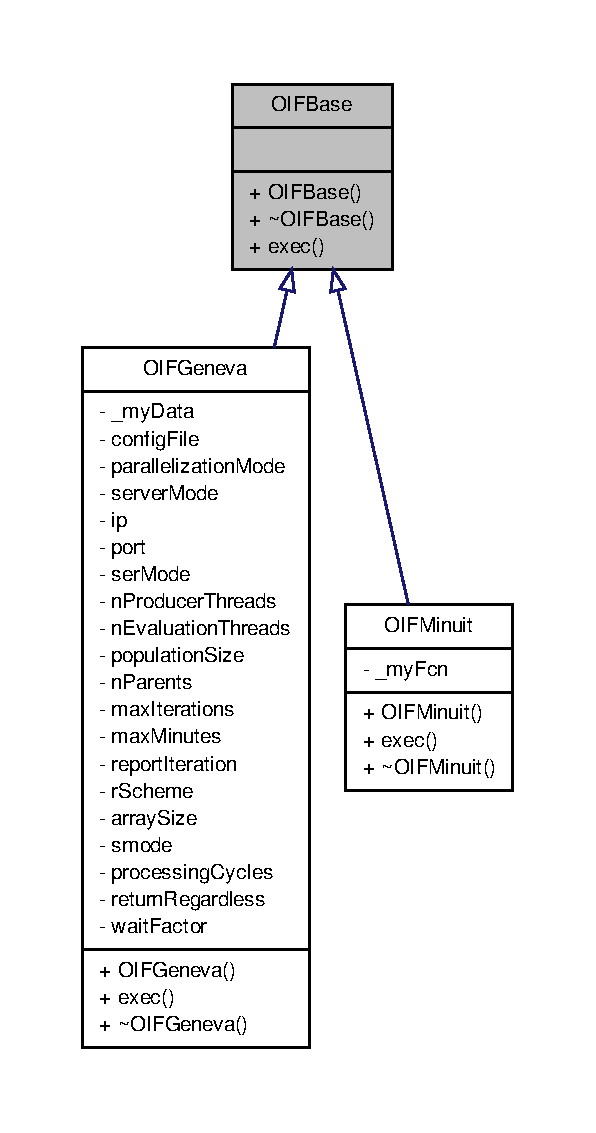
\includegraphics[width=286pt]{db/d8d/classOIFBase__inherit__graph}
\end{center}
\end{figure}
\subsection*{Public Member Functions}
\begin{DoxyCompactItemize}
\item 
\hyperlink{classOIFBase_a1e964e846b32437d0009bbd924caae72}{OIFBase} ()
\item 
virtual \hyperlink{classOIFBase_ad39d706bbab59c376437b592db1164ff}{$\sim$OIFBase} ()
\item 
virtual const double \hyperlink{classOIFBase_acc6067869ca4adf70f00075196c5ebdf}{exec} (unsigned int Npar, double $\ast$par, double $\ast$min, double $\ast$max, double $\ast$err)=0
\end{DoxyCompactItemize}


\subsection{Detailed Description}
Optimizer Interface Base-\/Class. 

\subsection{Constructor \& Destructor Documentation}
\hypertarget{classOIFBase_a1e964e846b32437d0009bbd924caae72}{
\index{OIFBase@{OIFBase}!OIFBase@{OIFBase}}
\index{OIFBase@{OIFBase}!OIFBase@{OIFBase}}
\subsubsection[{OIFBase}]{\setlength{\rightskip}{0pt plus 5cm}OIFBase::OIFBase (
\begin{DoxyParamCaption}
{}
\end{DoxyParamCaption}
)\hspace{0.3cm}{\ttfamily  \mbox{[}inline\mbox{]}}}}
\label{d0/d31/classOIFBase_a1e964e846b32437d0009bbd924caae72}
\hypertarget{classOIFBase_ad39d706bbab59c376437b592db1164ff}{
\index{OIFBase@{OIFBase}!$\sim$OIFBase@{$\sim$OIFBase}}
\index{$\sim$OIFBase@{$\sim$OIFBase}!OIFBase@{OIFBase}}
\subsubsection[{$\sim$OIFBase}]{\setlength{\rightskip}{0pt plus 5cm}virtual OIFBase::$\sim$OIFBase (
\begin{DoxyParamCaption}
{}
\end{DoxyParamCaption}
)\hspace{0.3cm}{\ttfamily  \mbox{[}inline, virtual\mbox{]}}}}
\label{d0/d31/classOIFBase_ad39d706bbab59c376437b592db1164ff}


\subsection{Member Function Documentation}
\hypertarget{classOIFBase_acc6067869ca4adf70f00075196c5ebdf}{
\index{OIFBase@{OIFBase}!exec@{exec}}
\index{exec@{exec}!OIFBase@{OIFBase}}
\subsubsection[{exec}]{\setlength{\rightskip}{0pt plus 5cm}virtual const double OIFBase::exec (
\begin{DoxyParamCaption}
\item[{unsigned int}]{Npar, }
\item[{double $\ast$}]{par, }
\item[{double $\ast$}]{min, }
\item[{double $\ast$}]{max, }
\item[{double $\ast$}]{err}
\end{DoxyParamCaption}
)\hspace{0.3cm}{\ttfamily  \mbox{[}pure virtual\mbox{]}}}}
\label{d0/d31/classOIFBase_acc6067869ca4adf70f00075196c5ebdf}


Implemented in \hyperlink{classOIFGeneva_a1a5cf2ace477bd40ce1c4848365a2f13}{OIFGeneva}, and \hyperlink{classOIFMinuit_a6a8ff974bdddf918ab2abb5a5a7810b6}{OIFMinuit}.



The documentation for this class was generated from the following file:\begin{DoxyCompactItemize}
\item 
Core/\hyperlink{OIFBase_8hpp}{OIFBase.hpp}\end{DoxyCompactItemize}

\hypertarget{classOIFData}{
\section{OIFData Class Reference}
\label{d1/d4f/classOIFData}\index{OIFData@{OIFData}}
}


Optimizer Data Base-\/Class.  




{\ttfamily \#include $<$OIFData.hpp$>$}



Inheritance diagram for OIFData:
\nopagebreak
\begin{figure}[H]
\begin{center}
\leavevmode
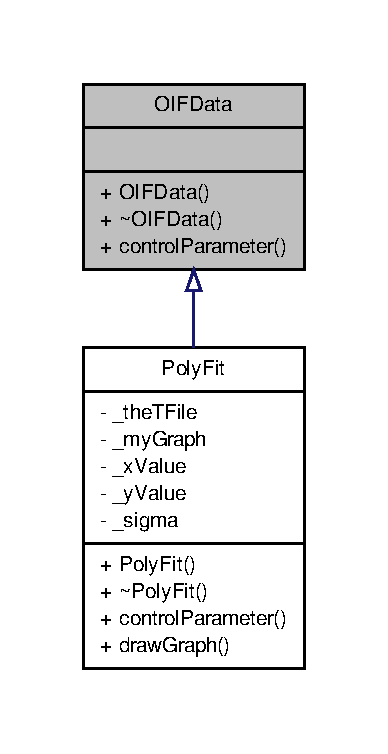
\includegraphics[width=186pt]{d9/d48/classOIFData__inherit__graph}
\end{center}
\end{figure}
\subsection*{Public Member Functions}
\begin{DoxyCompactItemize}
\item 
\hyperlink{classOIFData_a11151212f0897c14c0b81b0b55939473}{OIFData} ()
\item 
virtual \hyperlink{classOIFData_ab7126c43d4911e022db3033996fc345c}{$\sim$OIFData} ()
\item 
virtual double \hyperlink{classOIFData_adb5b2e9a28b1767f07ccb8737211ff4f}{controlParameter} (const std::vector$<$ double $>$ \&minPar)=0
\end{DoxyCompactItemize}


\subsection{Detailed Description}
Optimizer Data Base-\/Class. 

\subsection{Constructor \& Destructor Documentation}
\hypertarget{classOIFData_a11151212f0897c14c0b81b0b55939473}{
\index{OIFData@{OIFData}!OIFData@{OIFData}}
\index{OIFData@{OIFData}!OIFData@{OIFData}}
\subsubsection[{OIFData}]{\setlength{\rightskip}{0pt plus 5cm}OIFData::OIFData (
\begin{DoxyParamCaption}
{}
\end{DoxyParamCaption}
)\hspace{0.3cm}{\ttfamily  \mbox{[}inline\mbox{]}}}}
\label{d1/d4f/classOIFData_a11151212f0897c14c0b81b0b55939473}
\hypertarget{classOIFData_ab7126c43d4911e022db3033996fc345c}{
\index{OIFData@{OIFData}!$\sim$OIFData@{$\sim$OIFData}}
\index{$\sim$OIFData@{$\sim$OIFData}!OIFData@{OIFData}}
\subsubsection[{$\sim$OIFData}]{\setlength{\rightskip}{0pt plus 5cm}virtual OIFData::$\sim$OIFData (
\begin{DoxyParamCaption}
{}
\end{DoxyParamCaption}
)\hspace{0.3cm}{\ttfamily  \mbox{[}inline, virtual\mbox{]}}}}
\label{d1/d4f/classOIFData_ab7126c43d4911e022db3033996fc345c}


\subsection{Member Function Documentation}
\hypertarget{classOIFData_adb5b2e9a28b1767f07ccb8737211ff4f}{
\index{OIFData@{OIFData}!controlParameter@{controlParameter}}
\index{controlParameter@{controlParameter}!OIFData@{OIFData}}
\subsubsection[{controlParameter}]{\setlength{\rightskip}{0pt plus 5cm}virtual double OIFData::controlParameter (
\begin{DoxyParamCaption}
\item[{const std::vector$<$ double $>$ \&}]{minPar}
\end{DoxyParamCaption}
)\hspace{0.3cm}{\ttfamily  \mbox{[}pure virtual\mbox{]}}}}
\label{d1/d4f/classOIFData_adb5b2e9a28b1767f07ccb8737211ff4f}


Implemented in \hyperlink{classPolyFit_a5e7833b86023f7497b548711777bc273}{PolyFit}.



The documentation for this class was generated from the following file:\begin{DoxyCompactItemize}
\item 
Core/\hyperlink{OIFData_8hpp}{OIFData.hpp}\end{DoxyCompactItemize}

\hypertarget{classOIFGeneva}{
\section{OIFGeneva Class Reference}
\label{d4/dce/classOIFGeneva}\index{OIFGeneva@{OIFGeneva}}
}


Wrapper of the Geneva Optimizer library.  




{\ttfamily \#include $<$OIFGeneva.hpp$>$}



Inheritance diagram for OIFGeneva:\nopagebreak
\begin{figure}[H]
\begin{center}
\leavevmode
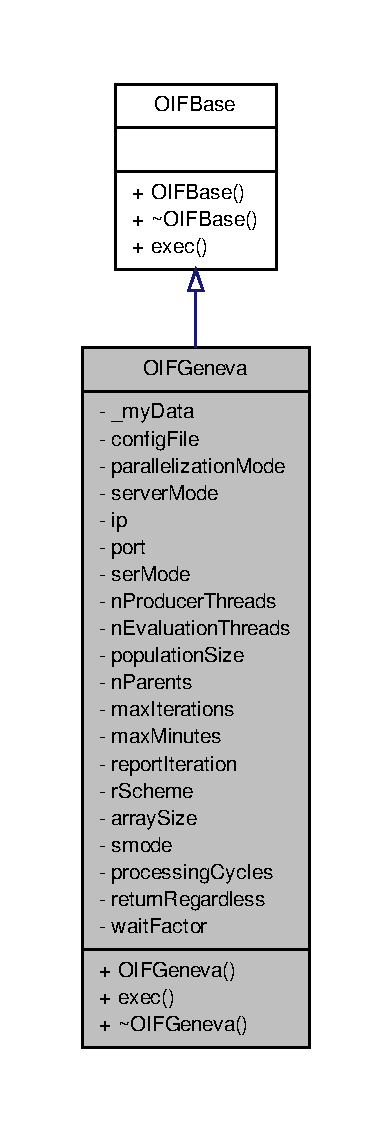
\includegraphics[width=188pt]{d9/d88/classOIFGeneva__inherit__graph}
\end{center}
\end{figure}


Collaboration diagram for OIFGeneva:\nopagebreak
\begin{figure}[H]
\begin{center}
\leavevmode
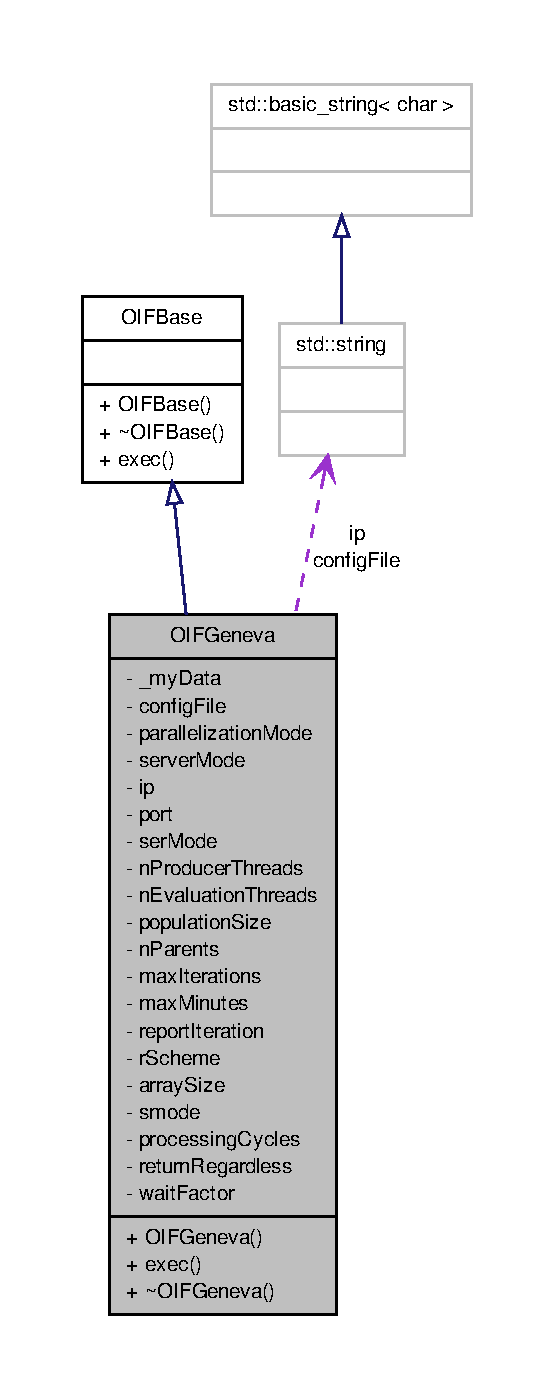
\includegraphics[height=600pt]{df/d29/classOIFGeneva__coll__graph}
\end{center}
\end{figure}
\subsection*{Public Member Functions}
\begin{DoxyCompactItemize}
\item 
\hyperlink{classOIFGeneva_a89e83a814e6571cb875d18cdedf42449}{OIFGeneva} (std::shared\_\-ptr$<$ \hyperlink{classOIFData}{OIFData} $>$ theData, std::string inConfigFile=\char`\"{}test/GStartProject.cfg\char`\"{}, boost::uint16\_\-t inparallelizationMode=1, bool inserverMode=false, std::string inip=\char`\"{}localhost\char`\"{}, unsigned short inport=10000, Gem::Common::serializationMode inserMode=Gem::Common::SERIALIZATIONMODE\_\-TEXT)
\begin{DoxyCompactList}\small\item\em Default Constructor (0x0) \end{DoxyCompactList}\item 
virtual const double \hyperlink{classOIFGeneva_a1a5cf2ace477bd40ce1c4848365a2f13}{exec} (unsigned int Npar, double $\ast$par, double $\ast$min, double $\ast$max, double $\ast$err)
\item 
virtual \hyperlink{classOIFGeneva_a72a8b0d30f8ef7d1d7dbe51a15a412e3}{$\sim$OIFGeneva} ()
\end{DoxyCompactItemize}
\subsection*{Private Attributes}
\begin{DoxyCompactItemize}
\item 
std::shared\_\-ptr$<$ \hyperlink{classOIFData}{OIFData} $>$ \hyperlink{classOIFGeneva_a6f384385ad5eebc149aa9cc84665c271}{\_\-myData}
\item 
std::string \hyperlink{classOIFGeneva_abf5610433384454ae4884b2f17f01f01}{configFile}
\item 
boost::uint16\_\-t \hyperlink{classOIFGeneva_ae51bcfad038f5365a2ff5c4d0691e05b}{parallelizationMode}
\item 
bool \hyperlink{classOIFGeneva_a12fed8d5df83853111e8e9bba2b00b5e}{serverMode}
\item 
std::string \hyperlink{classOIFGeneva_a24b10918d314755d3c566ea8c17b2bc1}{ip}
\item 
unsigned short \hyperlink{classOIFGeneva_a49edc5e8fefa9137eab821b81f8015b1}{port}
\item 
Gem::Common::serializationMode \hyperlink{classOIFGeneva_aaad7df3d69cbe6399123820e7fef2a3c}{serMode}
\item 
boost::uint16\_\-t \hyperlink{classOIFGeneva_a4b3bfbf12d2911a081fc7c5feb9c4ae7}{nProducerThreads}
\item 
boost::uint16\_\-t \hyperlink{classOIFGeneva_a9afb57f9439eddc693b06456c7f1a4a6}{nEvaluationThreads}
\item 
std::size\_\-t \hyperlink{classOIFGeneva_a9797a7ec73f3bf9b192799813f601600}{populationSize}
\item 
std::size\_\-t \hyperlink{classOIFGeneva_a01cfc180dd253ea8767446e4116f8bb2}{nParents}
\item 
boost::uint32\_\-t \hyperlink{classOIFGeneva_ae2a0cd2de953edc56ffa0dbb743fc9af}{maxIterations}
\item 
long \hyperlink{classOIFGeneva_a48b49d12e4ecd4a0e19b31692224f2a7}{maxMinutes}
\item 
boost::uint32\_\-t \hyperlink{classOIFGeneva_a4419a9af665e5589174b4442fb3e44b9}{reportIteration}
\item 
Gem::Geneva::recoScheme \hyperlink{classOIFGeneva_a84d9c1da4a30943abe44cbc58162755f}{rScheme}
\item 
std::size\_\-t \hyperlink{classOIFGeneva_ae17ccd19943bfe1ced5f7b0373c36ee9}{arraySize}
\item 
Gem::Geneva::sortingMode \hyperlink{classOIFGeneva_a74949f91a856d291c760b6668ace8275}{smode}
\item 
boost::uint32\_\-t \hyperlink{classOIFGeneva_a1e194ecfec04056b27e32205839a3f60}{processingCycles}
\item 
bool \hyperlink{classOIFGeneva_a812f07c15fdfda372b6fb82ad9d3795a}{returnRegardless}
\item 
boost::uint32\_\-t \hyperlink{classOIFGeneva_ad40b4a27317aacf88a920b07c23010ab}{waitFactor}
\end{DoxyCompactItemize}


\subsection{Detailed Description}
Wrapper of the Geneva Optimizer library. 

\subsection{Constructor \& Destructor Documentation}
\hypertarget{classOIFGeneva_a89e83a814e6571cb875d18cdedf42449}{
\index{OIFGeneva@{OIFGeneva}!OIFGeneva@{OIFGeneva}}
\index{OIFGeneva@{OIFGeneva}!OIFGeneva@{OIFGeneva}}
\subsubsection[{OIFGeneva}]{\setlength{\rightskip}{0pt plus 5cm}OIFGeneva::OIFGeneva (
\begin{DoxyParamCaption}
\item[{std::shared\_\-ptr$<$ {\bf OIFData} $>$}]{theData, }
\item[{std::string}]{inConfigFile = {\ttfamily \char`\"{}test/GStartProject.cfg\char`\"{}}, }
\item[{boost::uint16\_\-t}]{inparallelizationMode = {\ttfamily 1}, }
\item[{bool}]{inserverMode = {\ttfamily false}, }
\item[{std::string}]{inip = {\ttfamily \char`\"{}localhost\char`\"{}}, }
\item[{unsigned short}]{inport = {\ttfamily 10000}, }
\item[{Gem::Common::serializationMode}]{inserMode = {\ttfamily Gem::Common::SERIALIZATIONMODE\_\-TEXT}}
\end{DoxyParamCaption}
)}}
\label{d4/dce/classOIFGeneva_a89e83a814e6571cb875d18cdedf42449}


Default Constructor (0x0) 

\hypertarget{classOIFGeneva_a72a8b0d30f8ef7d1d7dbe51a15a412e3}{
\index{OIFGeneva@{OIFGeneva}!$\sim$OIFGeneva@{$\sim$OIFGeneva}}
\index{$\sim$OIFGeneva@{$\sim$OIFGeneva}!OIFGeneva@{OIFGeneva}}
\subsubsection[{$\sim$OIFGeneva}]{\setlength{\rightskip}{0pt plus 5cm}OIFGeneva::$\sim$OIFGeneva (
\begin{DoxyParamCaption}
{}
\end{DoxyParamCaption}
)\hspace{0.3cm}{\ttfamily  \mbox{[}virtual\mbox{]}}}}
\label{d4/dce/classOIFGeneva_a72a8b0d30f8ef7d1d7dbe51a15a412e3}
Destructor 

\subsection{Member Function Documentation}
\hypertarget{classOIFGeneva_a1a5cf2ace477bd40ce1c4848365a2f13}{
\index{OIFGeneva@{OIFGeneva}!exec@{exec}}
\index{exec@{exec}!OIFGeneva@{OIFGeneva}}
\subsubsection[{exec}]{\setlength{\rightskip}{0pt plus 5cm}const double OIFGeneva::exec (
\begin{DoxyParamCaption}
\item[{unsigned int}]{Npar, }
\item[{double $\ast$}]{par, }
\item[{double $\ast$}]{min, }
\item[{double $\ast$}]{max, }
\item[{double $\ast$}]{err}
\end{DoxyParamCaption}
)\hspace{0.3cm}{\ttfamily  \mbox{[}virtual\mbox{]}}}}
\label{d4/dce/classOIFGeneva_a1a5cf2ace477bd40ce1c4848365a2f13}


Implements \hyperlink{classOIFBase_acc6067869ca4adf70f00075196c5ebdf}{OIFBase}.



\subsection{Member Data Documentation}
\hypertarget{classOIFGeneva_a6f384385ad5eebc149aa9cc84665c271}{
\index{OIFGeneva@{OIFGeneva}!\_\-myData@{\_\-myData}}
\index{\_\-myData@{\_\-myData}!OIFGeneva@{OIFGeneva}}
\subsubsection[{\_\-myData}]{\setlength{\rightskip}{0pt plus 5cm}std::shared\_\-ptr$<${\bf OIFData}$>$ {\bf OIFGeneva::\_\-myData}\hspace{0.3cm}{\ttfamily  \mbox{[}private\mbox{]}}}}
\label{d4/dce/classOIFGeneva_a6f384385ad5eebc149aa9cc84665c271}
\hypertarget{classOIFGeneva_ae17ccd19943bfe1ced5f7b0373c36ee9}{
\index{OIFGeneva@{OIFGeneva}!arraySize@{arraySize}}
\index{arraySize@{arraySize}!OIFGeneva@{OIFGeneva}}
\subsubsection[{arraySize}]{\setlength{\rightskip}{0pt plus 5cm}std::size\_\-t {\bf OIFGeneva::arraySize}\hspace{0.3cm}{\ttfamily  \mbox{[}private\mbox{]}}}}
\label{d4/dce/classOIFGeneva_ae17ccd19943bfe1ced5f7b0373c36ee9}
\hypertarget{classOIFGeneva_abf5610433384454ae4884b2f17f01f01}{
\index{OIFGeneva@{OIFGeneva}!configFile@{configFile}}
\index{configFile@{configFile}!OIFGeneva@{OIFGeneva}}
\subsubsection[{configFile}]{\setlength{\rightskip}{0pt plus 5cm}std::string {\bf OIFGeneva::configFile}\hspace{0.3cm}{\ttfamily  \mbox{[}private\mbox{]}}}}
\label{d4/dce/classOIFGeneva_abf5610433384454ae4884b2f17f01f01}
\hypertarget{classOIFGeneva_a24b10918d314755d3c566ea8c17b2bc1}{
\index{OIFGeneva@{OIFGeneva}!ip@{ip}}
\index{ip@{ip}!OIFGeneva@{OIFGeneva}}
\subsubsection[{ip}]{\setlength{\rightskip}{0pt plus 5cm}std::string {\bf OIFGeneva::ip}\hspace{0.3cm}{\ttfamily  \mbox{[}private\mbox{]}}}}
\label{d4/dce/classOIFGeneva_a24b10918d314755d3c566ea8c17b2bc1}
\hypertarget{classOIFGeneva_ae2a0cd2de953edc56ffa0dbb743fc9af}{
\index{OIFGeneva@{OIFGeneva}!maxIterations@{maxIterations}}
\index{maxIterations@{maxIterations}!OIFGeneva@{OIFGeneva}}
\subsubsection[{maxIterations}]{\setlength{\rightskip}{0pt plus 5cm}boost::uint32\_\-t {\bf OIFGeneva::maxIterations}\hspace{0.3cm}{\ttfamily  \mbox{[}private\mbox{]}}}}
\label{d4/dce/classOIFGeneva_ae2a0cd2de953edc56ffa0dbb743fc9af}
\hypertarget{classOIFGeneva_a48b49d12e4ecd4a0e19b31692224f2a7}{
\index{OIFGeneva@{OIFGeneva}!maxMinutes@{maxMinutes}}
\index{maxMinutes@{maxMinutes}!OIFGeneva@{OIFGeneva}}
\subsubsection[{maxMinutes}]{\setlength{\rightskip}{0pt plus 5cm}long {\bf OIFGeneva::maxMinutes}\hspace{0.3cm}{\ttfamily  \mbox{[}private\mbox{]}}}}
\label{d4/dce/classOIFGeneva_a48b49d12e4ecd4a0e19b31692224f2a7}
\hypertarget{classOIFGeneva_a9afb57f9439eddc693b06456c7f1a4a6}{
\index{OIFGeneva@{OIFGeneva}!nEvaluationThreads@{nEvaluationThreads}}
\index{nEvaluationThreads@{nEvaluationThreads}!OIFGeneva@{OIFGeneva}}
\subsubsection[{nEvaluationThreads}]{\setlength{\rightskip}{0pt plus 5cm}boost::uint16\_\-t {\bf OIFGeneva::nEvaluationThreads}\hspace{0.3cm}{\ttfamily  \mbox{[}private\mbox{]}}}}
\label{d4/dce/classOIFGeneva_a9afb57f9439eddc693b06456c7f1a4a6}
\hypertarget{classOIFGeneva_a01cfc180dd253ea8767446e4116f8bb2}{
\index{OIFGeneva@{OIFGeneva}!nParents@{nParents}}
\index{nParents@{nParents}!OIFGeneva@{OIFGeneva}}
\subsubsection[{nParents}]{\setlength{\rightskip}{0pt plus 5cm}std::size\_\-t {\bf OIFGeneva::nParents}\hspace{0.3cm}{\ttfamily  \mbox{[}private\mbox{]}}}}
\label{d4/dce/classOIFGeneva_a01cfc180dd253ea8767446e4116f8bb2}
\hypertarget{classOIFGeneva_a4b3bfbf12d2911a081fc7c5feb9c4ae7}{
\index{OIFGeneva@{OIFGeneva}!nProducerThreads@{nProducerThreads}}
\index{nProducerThreads@{nProducerThreads}!OIFGeneva@{OIFGeneva}}
\subsubsection[{nProducerThreads}]{\setlength{\rightskip}{0pt plus 5cm}boost::uint16\_\-t {\bf OIFGeneva::nProducerThreads}\hspace{0.3cm}{\ttfamily  \mbox{[}private\mbox{]}}}}
\label{d4/dce/classOIFGeneva_a4b3bfbf12d2911a081fc7c5feb9c4ae7}
\hypertarget{classOIFGeneva_ae51bcfad038f5365a2ff5c4d0691e05b}{
\index{OIFGeneva@{OIFGeneva}!parallelizationMode@{parallelizationMode}}
\index{parallelizationMode@{parallelizationMode}!OIFGeneva@{OIFGeneva}}
\subsubsection[{parallelizationMode}]{\setlength{\rightskip}{0pt plus 5cm}boost::uint16\_\-t {\bf OIFGeneva::parallelizationMode}\hspace{0.3cm}{\ttfamily  \mbox{[}private\mbox{]}}}}
\label{d4/dce/classOIFGeneva_ae51bcfad038f5365a2ff5c4d0691e05b}
\hypertarget{classOIFGeneva_a9797a7ec73f3bf9b192799813f601600}{
\index{OIFGeneva@{OIFGeneva}!populationSize@{populationSize}}
\index{populationSize@{populationSize}!OIFGeneva@{OIFGeneva}}
\subsubsection[{populationSize}]{\setlength{\rightskip}{0pt plus 5cm}std::size\_\-t {\bf OIFGeneva::populationSize}\hspace{0.3cm}{\ttfamily  \mbox{[}private\mbox{]}}}}
\label{d4/dce/classOIFGeneva_a9797a7ec73f3bf9b192799813f601600}
\hypertarget{classOIFGeneva_a49edc5e8fefa9137eab821b81f8015b1}{
\index{OIFGeneva@{OIFGeneva}!port@{port}}
\index{port@{port}!OIFGeneva@{OIFGeneva}}
\subsubsection[{port}]{\setlength{\rightskip}{0pt plus 5cm}unsigned short {\bf OIFGeneva::port}\hspace{0.3cm}{\ttfamily  \mbox{[}private\mbox{]}}}}
\label{d4/dce/classOIFGeneva_a49edc5e8fefa9137eab821b81f8015b1}
\hypertarget{classOIFGeneva_a1e194ecfec04056b27e32205839a3f60}{
\index{OIFGeneva@{OIFGeneva}!processingCycles@{processingCycles}}
\index{processingCycles@{processingCycles}!OIFGeneva@{OIFGeneva}}
\subsubsection[{processingCycles}]{\setlength{\rightskip}{0pt plus 5cm}boost::uint32\_\-t {\bf OIFGeneva::processingCycles}\hspace{0.3cm}{\ttfamily  \mbox{[}private\mbox{]}}}}
\label{d4/dce/classOIFGeneva_a1e194ecfec04056b27e32205839a3f60}
\hypertarget{classOIFGeneva_a4419a9af665e5589174b4442fb3e44b9}{
\index{OIFGeneva@{OIFGeneva}!reportIteration@{reportIteration}}
\index{reportIteration@{reportIteration}!OIFGeneva@{OIFGeneva}}
\subsubsection[{reportIteration}]{\setlength{\rightskip}{0pt plus 5cm}boost::uint32\_\-t {\bf OIFGeneva::reportIteration}\hspace{0.3cm}{\ttfamily  \mbox{[}private\mbox{]}}}}
\label{d4/dce/classOIFGeneva_a4419a9af665e5589174b4442fb3e44b9}
\hypertarget{classOIFGeneva_a812f07c15fdfda372b6fb82ad9d3795a}{
\index{OIFGeneva@{OIFGeneva}!returnRegardless@{returnRegardless}}
\index{returnRegardless@{returnRegardless}!OIFGeneva@{OIFGeneva}}
\subsubsection[{returnRegardless}]{\setlength{\rightskip}{0pt plus 5cm}bool {\bf OIFGeneva::returnRegardless}\hspace{0.3cm}{\ttfamily  \mbox{[}private\mbox{]}}}}
\label{d4/dce/classOIFGeneva_a812f07c15fdfda372b6fb82ad9d3795a}
\hypertarget{classOIFGeneva_a84d9c1da4a30943abe44cbc58162755f}{
\index{OIFGeneva@{OIFGeneva}!rScheme@{rScheme}}
\index{rScheme@{rScheme}!OIFGeneva@{OIFGeneva}}
\subsubsection[{rScheme}]{\setlength{\rightskip}{0pt plus 5cm}Gem::Geneva::recoScheme {\bf OIFGeneva::rScheme}\hspace{0.3cm}{\ttfamily  \mbox{[}private\mbox{]}}}}
\label{d4/dce/classOIFGeneva_a84d9c1da4a30943abe44cbc58162755f}
\hypertarget{classOIFGeneva_aaad7df3d69cbe6399123820e7fef2a3c}{
\index{OIFGeneva@{OIFGeneva}!serMode@{serMode}}
\index{serMode@{serMode}!OIFGeneva@{OIFGeneva}}
\subsubsection[{serMode}]{\setlength{\rightskip}{0pt plus 5cm}Gem::Common::serializationMode {\bf OIFGeneva::serMode}\hspace{0.3cm}{\ttfamily  \mbox{[}private\mbox{]}}}}
\label{d4/dce/classOIFGeneva_aaad7df3d69cbe6399123820e7fef2a3c}
\hypertarget{classOIFGeneva_a12fed8d5df83853111e8e9bba2b00b5e}{
\index{OIFGeneva@{OIFGeneva}!serverMode@{serverMode}}
\index{serverMode@{serverMode}!OIFGeneva@{OIFGeneva}}
\subsubsection[{serverMode}]{\setlength{\rightskip}{0pt plus 5cm}bool {\bf OIFGeneva::serverMode}\hspace{0.3cm}{\ttfamily  \mbox{[}private\mbox{]}}}}
\label{d4/dce/classOIFGeneva_a12fed8d5df83853111e8e9bba2b00b5e}
\hypertarget{classOIFGeneva_a74949f91a856d291c760b6668ace8275}{
\index{OIFGeneva@{OIFGeneva}!smode@{smode}}
\index{smode@{smode}!OIFGeneva@{OIFGeneva}}
\subsubsection[{smode}]{\setlength{\rightskip}{0pt plus 5cm}Gem::Geneva::sortingMode {\bf OIFGeneva::smode}\hspace{0.3cm}{\ttfamily  \mbox{[}private\mbox{]}}}}
\label{d4/dce/classOIFGeneva_a74949f91a856d291c760b6668ace8275}
\hypertarget{classOIFGeneva_ad40b4a27317aacf88a920b07c23010ab}{
\index{OIFGeneva@{OIFGeneva}!waitFactor@{waitFactor}}
\index{waitFactor@{waitFactor}!OIFGeneva@{OIFGeneva}}
\subsubsection[{waitFactor}]{\setlength{\rightskip}{0pt plus 5cm}boost::uint32\_\-t {\bf OIFGeneva::waitFactor}\hspace{0.3cm}{\ttfamily  \mbox{[}private\mbox{]}}}}
\label{d4/dce/classOIFGeneva_ad40b4a27317aacf88a920b07c23010ab}


The documentation for this class was generated from the following files:\begin{DoxyCompactItemize}
\item 
OIFGeneva/\hyperlink{OIFGeneva_8hpp}{OIFGeneva.hpp}\item 
OIFGeneva/\hyperlink{OIFGeneva_8cpp}{OIFGeneva.cpp}\end{DoxyCompactItemize}

\hypertarget{classOIFMinuit}{
\section{OIFMinuit Class Reference}
\label{d5/db7/classOIFMinuit}\index{OIFMinuit@{OIFMinuit}}
}


Wrapper of the Minuit2 Optimizer library.  




{\ttfamily \#include $<$OIFMinuit.hpp$>$}



Inheritance diagram for OIFMinuit:
\nopagebreak
\begin{figure}[H]
\begin{center}
\leavevmode
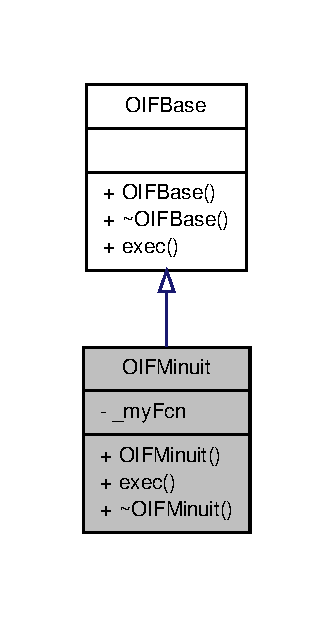
\includegraphics[width=160pt]{dc/daa/classOIFMinuit__inherit__graph}
\end{center}
\end{figure}


Collaboration diagram for OIFMinuit:
\nopagebreak
\begin{figure}[H]
\begin{center}
\leavevmode
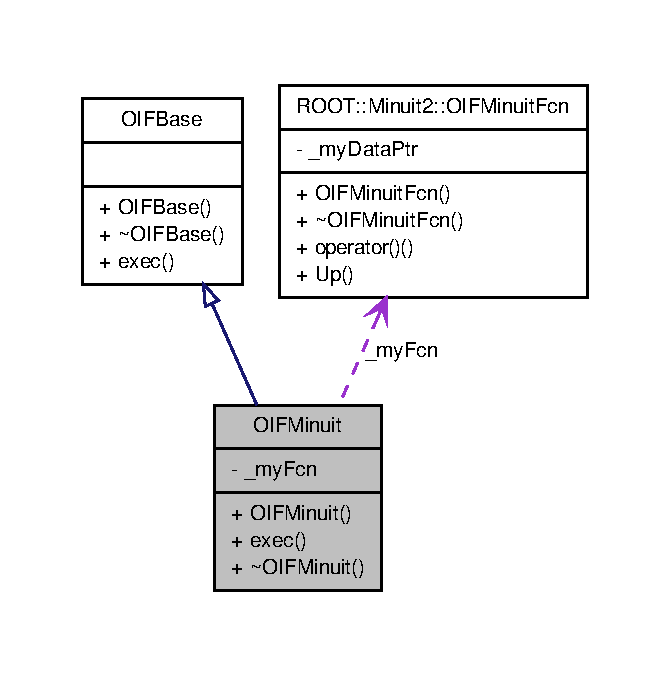
\includegraphics[width=322pt]{d4/da7/classOIFMinuit__coll__graph}
\end{center}
\end{figure}
\subsection*{Public Member Functions}
\begin{DoxyCompactItemize}
\item 
\hyperlink{classOIFMinuit_a24a4245e7e2775c199a6d60717d8027d}{OIFMinuit} (std::shared\_\-ptr$<$ \hyperlink{classOIFData}{OIFData} $>$ theData)
\begin{DoxyCompactList}\small\item\em Default Constructor (0x0) \end{DoxyCompactList}\item 
virtual const double \hyperlink{classOIFMinuit_a6a8ff974bdddf918ab2abb5a5a7810b6}{exec} (unsigned int Npar, double $\ast$par, double $\ast$min, double $\ast$max, double $\ast$err)
\item 
virtual \hyperlink{classOIFMinuit_ac0653bc60bb66da10970480d76596975}{$\sim$OIFMinuit} ()
\end{DoxyCompactItemize}
\subsection*{Private Attributes}
\begin{DoxyCompactItemize}
\item 
\hyperlink{classROOT_1_1Minuit2_1_1OIFMinuitFcn}{OIFMinuitFcn} \hyperlink{classOIFMinuit_ae4ec346c614ffd9881ab2c24f9024351}{\_\-myFcn}
\end{DoxyCompactItemize}


\subsection{Detailed Description}
Wrapper of the Minuit2 Optimizer library. 

\subsection{Constructor \& Destructor Documentation}
\hypertarget{classOIFMinuit_a24a4245e7e2775c199a6d60717d8027d}{
\index{OIFMinuit@{OIFMinuit}!OIFMinuit@{OIFMinuit}}
\index{OIFMinuit@{OIFMinuit}!OIFMinuit@{OIFMinuit}}
\subsubsection[{OIFMinuit}]{\setlength{\rightskip}{0pt plus 5cm}OIFMinuit::OIFMinuit (
\begin{DoxyParamCaption}
\item[{std::shared\_\-ptr$<$ {\bf OIFData} $>$}]{theData}
\end{DoxyParamCaption}
)}}
\label{d5/db7/classOIFMinuit_a24a4245e7e2775c199a6d60717d8027d}


Default Constructor (0x0) 

\hypertarget{classOIFMinuit_ac0653bc60bb66da10970480d76596975}{
\index{OIFMinuit@{OIFMinuit}!$\sim$OIFMinuit@{$\sim$OIFMinuit}}
\index{$\sim$OIFMinuit@{$\sim$OIFMinuit}!OIFMinuit@{OIFMinuit}}
\subsubsection[{$\sim$OIFMinuit}]{\setlength{\rightskip}{0pt plus 5cm}OIFMinuit::$\sim$OIFMinuit (
\begin{DoxyParamCaption}
{}
\end{DoxyParamCaption}
)\hspace{0.3cm}{\ttfamily  \mbox{[}virtual\mbox{]}}}}
\label{d5/db7/classOIFMinuit_ac0653bc60bb66da10970480d76596975}
Destructor 

\subsection{Member Function Documentation}
\hypertarget{classOIFMinuit_a6a8ff974bdddf918ab2abb5a5a7810b6}{
\index{OIFMinuit@{OIFMinuit}!exec@{exec}}
\index{exec@{exec}!OIFMinuit@{OIFMinuit}}
\subsubsection[{exec}]{\setlength{\rightskip}{0pt plus 5cm}const double OIFMinuit::exec (
\begin{DoxyParamCaption}
\item[{unsigned int}]{Npar, }
\item[{double $\ast$}]{par, }
\item[{double $\ast$}]{min, }
\item[{double $\ast$}]{max, }
\item[{double $\ast$}]{err}
\end{DoxyParamCaption}
)\hspace{0.3cm}{\ttfamily  \mbox{[}virtual\mbox{]}}}}
\label{d5/db7/classOIFMinuit_a6a8ff974bdddf918ab2abb5a5a7810b6}


Implements \hyperlink{classOIFBase_acc6067869ca4adf70f00075196c5ebdf}{OIFBase}.



\subsection{Member Data Documentation}
\hypertarget{classOIFMinuit_ae4ec346c614ffd9881ab2c24f9024351}{
\index{OIFMinuit@{OIFMinuit}!\_\-myFcn@{\_\-myFcn}}
\index{\_\-myFcn@{\_\-myFcn}!OIFMinuit@{OIFMinuit}}
\subsubsection[{\_\-myFcn}]{\setlength{\rightskip}{0pt plus 5cm}{\bf OIFMinuitFcn} {\bf OIFMinuit::\_\-myFcn}\hspace{0.3cm}{\ttfamily  \mbox{[}private\mbox{]}}}}
\label{d5/db7/classOIFMinuit_ae4ec346c614ffd9881ab2c24f9024351}


The documentation for this class was generated from the following files:\begin{DoxyCompactItemize}
\item 
OIFMinuit2/\hyperlink{OIFMinuit_8hpp}{OIFMinuit.hpp}\item 
OIFMinuit2/\hyperlink{OIFMinuit_8cpp}{OIFMinuit.cpp}\end{DoxyCompactItemize}

\hypertarget{classOIFMinuitFcn}{
\section{OIFMinuitFcn Class Reference}
\label{d5/d19/classOIFMinuitFcn}\index{OIFMinuitFcn@{OIFMinuitFcn}}
}


Minuit2 function to be optimized.  




{\ttfamily \#include $<$OIFMinuitFcn.hpp$>$}



\subsection{Detailed Description}
Minuit2 function to be optimized. 

The documentation for this class was generated from the following file:\begin{DoxyCompactItemize}
\item 
OIFMinuit2/\hyperlink{OIFMinuitFcn_8hpp}{OIFMinuitFcn.hpp}\end{DoxyCompactItemize}

\hypertarget{classROOT_1_1Minuit2_1_1OIFMinuitFcn}{
\section{ROOT::Minuit2::OIFMinuitFcn Class Reference}
\label{d3/dc7/classROOT_1_1Minuit2_1_1OIFMinuitFcn}\index{ROOT::Minuit2::OIFMinuitFcn@{ROOT::Minuit2::OIFMinuitFcn}}
}


{\ttfamily \#include $<$OIFMinuitFcn.hpp$>$}

\subsection*{Public Member Functions}
\begin{DoxyCompactItemize}
\item 
\hyperlink{classROOT_1_1Minuit2_1_1OIFMinuitFcn_aff2f5645420e8719ebc6415b04184433}{OIFMinuitFcn} (std::shared\_\-ptr$<$ \hyperlink{classOIFData}{OIFData} $>$ theData)
\item 
virtual \hyperlink{classROOT_1_1Minuit2_1_1OIFMinuitFcn_a6f933e4568fc0d8ad5a6d3d6ad2fd727}{$\sim$OIFMinuitFcn} ()
\item 
double \hyperlink{classROOT_1_1Minuit2_1_1OIFMinuitFcn_a7e83033d923f085fa8192c8952027f39}{operator()} (const std::vector$<$ double $>$ \&par) const 
\item 
double \hyperlink{classROOT_1_1Minuit2_1_1OIFMinuitFcn_a6f55d1c39778acd5bbed8e04e6f049e4}{Up} () const 
\end{DoxyCompactItemize}
\subsection*{Private Attributes}
\begin{DoxyCompactItemize}
\item 
std::shared\_\-ptr$<$ \hyperlink{classOIFData}{OIFData} $>$ \hyperlink{classROOT_1_1Minuit2_1_1OIFMinuitFcn_a0fd03437f3d07ab064773733efb8e4bf}{\_\-myDataPtr}
\end{DoxyCompactItemize}


\subsection{Constructor \& Destructor Documentation}
\hypertarget{classROOT_1_1Minuit2_1_1OIFMinuitFcn_aff2f5645420e8719ebc6415b04184433}{
\index{ROOT::Minuit2::OIFMinuitFcn@{ROOT::Minuit2::OIFMinuitFcn}!OIFMinuitFcn@{OIFMinuitFcn}}
\index{OIFMinuitFcn@{OIFMinuitFcn}!ROOT::Minuit2::OIFMinuitFcn@{ROOT::Minuit2::OIFMinuitFcn}}
\subsubsection[{OIFMinuitFcn}]{\setlength{\rightskip}{0pt plus 5cm}OIFMinuitFcn::OIFMinuitFcn (
\begin{DoxyParamCaption}
\item[{std::shared\_\-ptr$<$ {\bf OIFData} $>$}]{theData}
\end{DoxyParamCaption}
)}}
\label{d3/dc7/classROOT_1_1Minuit2_1_1OIFMinuitFcn_aff2f5645420e8719ebc6415b04184433}
\hypertarget{classROOT_1_1Minuit2_1_1OIFMinuitFcn_a6f933e4568fc0d8ad5a6d3d6ad2fd727}{
\index{ROOT::Minuit2::OIFMinuitFcn@{ROOT::Minuit2::OIFMinuitFcn}!$\sim$OIFMinuitFcn@{$\sim$OIFMinuitFcn}}
\index{$\sim$OIFMinuitFcn@{$\sim$OIFMinuitFcn}!ROOT::Minuit2::OIFMinuitFcn@{ROOT::Minuit2::OIFMinuitFcn}}
\subsubsection[{$\sim$OIFMinuitFcn}]{\setlength{\rightskip}{0pt plus 5cm}OIFMinuitFcn::$\sim$OIFMinuitFcn (
\begin{DoxyParamCaption}
{}
\end{DoxyParamCaption}
)\hspace{0.3cm}{\ttfamily  \mbox{[}virtual\mbox{]}}}}
\label{d3/dc7/classROOT_1_1Minuit2_1_1OIFMinuitFcn_a6f933e4568fc0d8ad5a6d3d6ad2fd727}


\subsection{Member Function Documentation}
\hypertarget{classROOT_1_1Minuit2_1_1OIFMinuitFcn_a7e83033d923f085fa8192c8952027f39}{
\index{ROOT::Minuit2::OIFMinuitFcn@{ROOT::Minuit2::OIFMinuitFcn}!operator()@{operator()}}
\index{operator()@{operator()}!ROOT::Minuit2::OIFMinuitFcn@{ROOT::Minuit2::OIFMinuitFcn}}
\subsubsection[{operator()}]{\setlength{\rightskip}{0pt plus 5cm}double OIFMinuitFcn::operator() (
\begin{DoxyParamCaption}
\item[{const std::vector$<$ double $>$ \&}]{par}
\end{DoxyParamCaption}
) const}}
\label{d3/dc7/classROOT_1_1Minuit2_1_1OIFMinuitFcn_a7e83033d923f085fa8192c8952027f39}
\hypertarget{classROOT_1_1Minuit2_1_1OIFMinuitFcn_a6f55d1c39778acd5bbed8e04e6f049e4}{
\index{ROOT::Minuit2::OIFMinuitFcn@{ROOT::Minuit2::OIFMinuitFcn}!Up@{Up}}
\index{Up@{Up}!ROOT::Minuit2::OIFMinuitFcn@{ROOT::Minuit2::OIFMinuitFcn}}
\subsubsection[{Up}]{\setlength{\rightskip}{0pt plus 5cm}double OIFMinuitFcn::Up (
\begin{DoxyParamCaption}
{}
\end{DoxyParamCaption}
) const}}
\label{d3/dc7/classROOT_1_1Minuit2_1_1OIFMinuitFcn_a6f55d1c39778acd5bbed8e04e6f049e4}


\subsection{Member Data Documentation}
\hypertarget{classROOT_1_1Minuit2_1_1OIFMinuitFcn_a0fd03437f3d07ab064773733efb8e4bf}{
\index{ROOT::Minuit2::OIFMinuitFcn@{ROOT::Minuit2::OIFMinuitFcn}!\_\-myDataPtr@{\_\-myDataPtr}}
\index{\_\-myDataPtr@{\_\-myDataPtr}!ROOT::Minuit2::OIFMinuitFcn@{ROOT::Minuit2::OIFMinuitFcn}}
\subsubsection[{\_\-myDataPtr}]{\setlength{\rightskip}{0pt plus 5cm}std::shared\_\-ptr$<${\bf OIFData}$>$ {\bf ROOT::Minuit2::OIFMinuitFcn::\_\-myDataPtr}\hspace{0.3cm}{\ttfamily  \mbox{[}private\mbox{]}}}}
\label{d3/dc7/classROOT_1_1Minuit2_1_1OIFMinuitFcn_a0fd03437f3d07ab064773733efb8e4bf}


The documentation for this class was generated from the following files:\begin{DoxyCompactItemize}
\item 
OIFMinuit2/\hyperlink{OIFMinuitFcn_8hpp}{OIFMinuitFcn.hpp}\item 
OIFMinuit2/\hyperlink{OIFMinuitFcn_8cpp}{OIFMinuitFcn.cpp}\end{DoxyCompactItemize}

\hypertarget{classPIFBase}{
\section{PIFBase Class Reference}
\label{d5/d3f/classPIFBase}\index{PIFBase@{PIFBase}}
}


Physics Interface Base-\/Class.  




{\ttfamily \#include $<$PIFBase.hpp$>$}

Inheritance diagram for PIFBase:\begin{figure}[H]
\begin{center}
\leavevmode
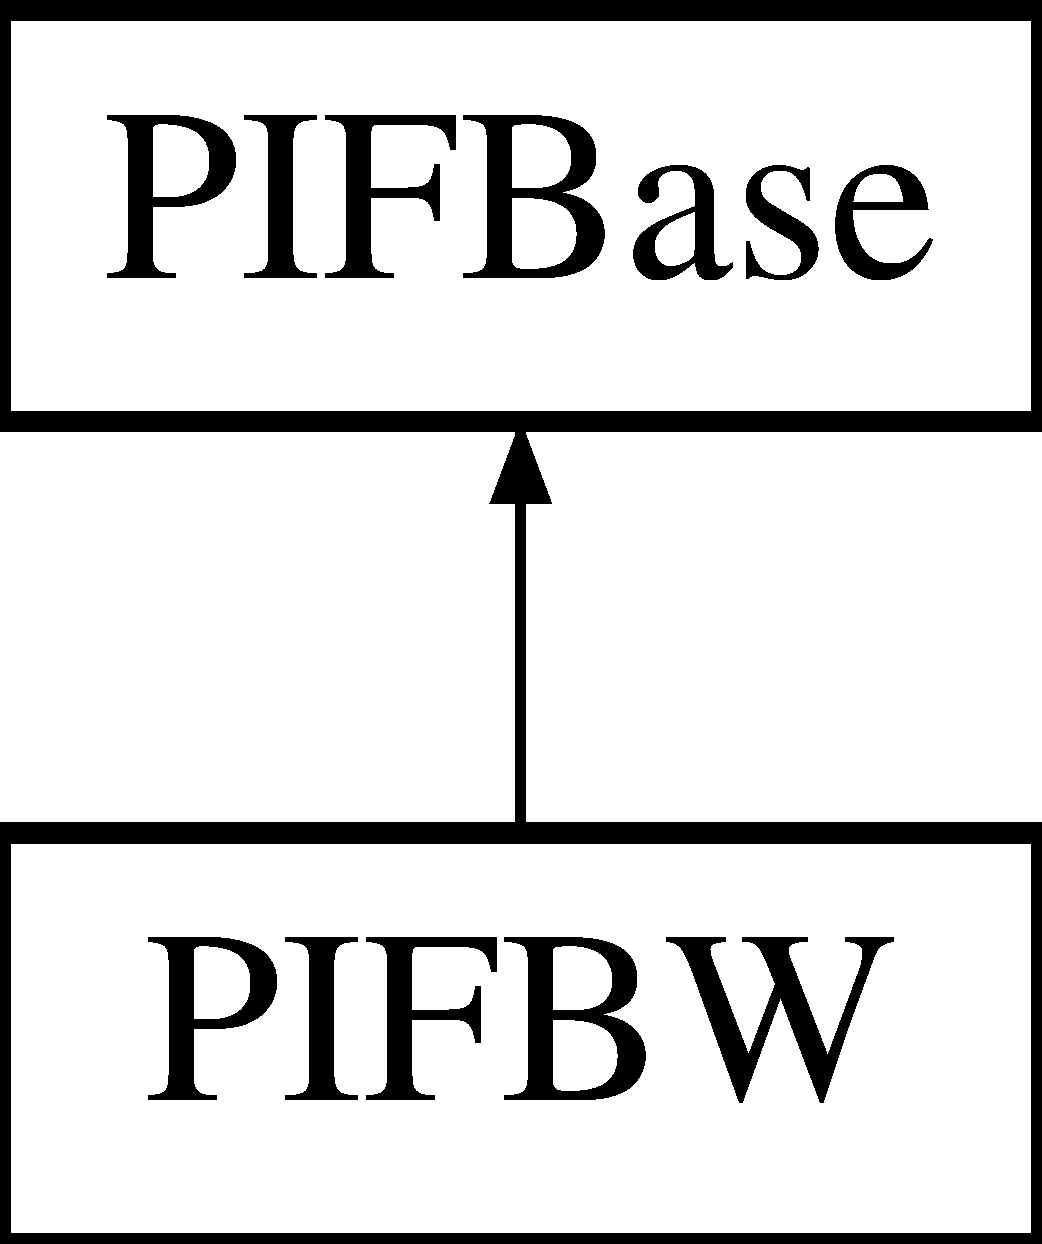
\includegraphics[height=2.000000cm]{d5/d3f/classPIFBase}
\end{center}
\end{figure}
\subsection*{Public Member Functions}
\begin{DoxyCompactItemize}
\item 
\hyperlink{classPIFBase_aa435256425c756fa92b2008ca7381a47}{PIFBase} ()
\item 
virtual \hyperlink{classPIFBase_a0b598b33b36f0ecda10c9cafe3c8e083}{$\sim$PIFBase} ()
\item 
virtual const double \hyperlink{classPIFBase_a7e0628a7d23475f2471fb9b7262659cf}{intensity} (double x, double M, double T)=0
\end{DoxyCompactItemize}


\subsection{Detailed Description}
Physics Interface Base-\/Class. 

\subsection{Constructor \& Destructor Documentation}
\hypertarget{classPIFBase_aa435256425c756fa92b2008ca7381a47}{
\index{PIFBase@{PIFBase}!PIFBase@{PIFBase}}
\index{PIFBase@{PIFBase}!PIFBase@{PIFBase}}
\subsubsection[{PIFBase}]{\setlength{\rightskip}{0pt plus 5cm}PIFBase::PIFBase (
\begin{DoxyParamCaption}
{}
\end{DoxyParamCaption}
)\hspace{0.3cm}{\ttfamily  \mbox{[}inline\mbox{]}}}}
\label{d5/d3f/classPIFBase_aa435256425c756fa92b2008ca7381a47}
\hypertarget{classPIFBase_a0b598b33b36f0ecda10c9cafe3c8e083}{
\index{PIFBase@{PIFBase}!$\sim$PIFBase@{$\sim$PIFBase}}
\index{$\sim$PIFBase@{$\sim$PIFBase}!PIFBase@{PIFBase}}
\subsubsection[{$\sim$PIFBase}]{\setlength{\rightskip}{0pt plus 5cm}virtual PIFBase::$\sim$PIFBase (
\begin{DoxyParamCaption}
{}
\end{DoxyParamCaption}
)\hspace{0.3cm}{\ttfamily  \mbox{[}inline, virtual\mbox{]}}}}
\label{d5/d3f/classPIFBase_a0b598b33b36f0ecda10c9cafe3c8e083}


\subsection{Member Function Documentation}
\hypertarget{classPIFBase_a7e0628a7d23475f2471fb9b7262659cf}{
\index{PIFBase@{PIFBase}!intensity@{intensity}}
\index{intensity@{intensity}!PIFBase@{PIFBase}}
\subsubsection[{intensity}]{\setlength{\rightskip}{0pt plus 5cm}virtual const double PIFBase::intensity (
\begin{DoxyParamCaption}
\item[{double}]{x, }
\item[{double}]{M, }
\item[{double}]{T}
\end{DoxyParamCaption}
)\hspace{0.3cm}{\ttfamily  \mbox{[}pure virtual\mbox{]}}}}
\label{d5/d3f/classPIFBase_a7e0628a7d23475f2471fb9b7262659cf}


Implemented in \hyperlink{classPIFBW_a044bc6c62245217b03abcd9d7b4e9e25}{PIFBW}.



The documentation for this class was generated from the following file:\begin{DoxyCompactItemize}
\item 
Core/\hyperlink{PIFBase_8hpp}{PIFBase.hpp}\end{DoxyCompactItemize}

\hypertarget{classPIFBW}{
\section{PIFBW Class Reference}
\label{d8/d58/classPIFBW}\index{PIFBW@{PIFBW}}
}


Physics Module with simple 1D Breit-\/Wigner.  




{\ttfamily \#include $<$PIFBW.hpp$>$}



Inheritance diagram for PIFBW:
\nopagebreak
\begin{figure}[H]
\begin{center}
\leavevmode
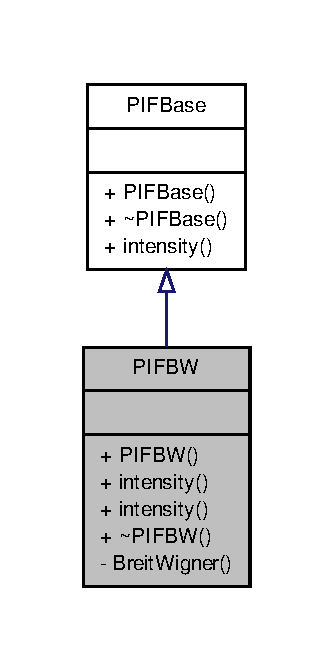
\includegraphics[width=160pt]{dc/de4/classPIFBW__inherit__graph}
\end{center}
\end{figure}


Collaboration diagram for PIFBW:
\nopagebreak
\begin{figure}[H]
\begin{center}
\leavevmode
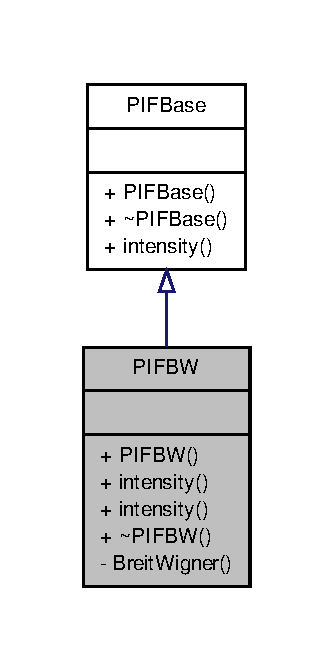
\includegraphics[width=160pt]{d3/d9b/classPIFBW__coll__graph}
\end{center}
\end{figure}
\subsection*{Public Member Functions}
\begin{DoxyCompactItemize}
\item 
\hyperlink{classPIFBW_a5dcb579e7810aedea4a13073415992e3}{PIFBW} ()
\begin{DoxyCompactList}\small\item\em Default Constructor (0x0) \end{DoxyCompactList}\item 
virtual const double \hyperlink{classPIFBW_a044bc6c62245217b03abcd9d7b4e9e25}{intensity} (double x, double M, double T)
\item 
virtual \hyperlink{classPIFBW_ae37b777b3d43bd6a78e07f8e971ba005}{$\sim$PIFBW} ()
\end{DoxyCompactItemize}
\subsection*{Private Member Functions}
\begin{DoxyCompactItemize}
\item 
const double \hyperlink{classPIFBW_a466dd8f3128a4ab2a9200ee44787dcef}{BreitWigner} (double x, double M, double T)
\end{DoxyCompactItemize}


\subsection{Detailed Description}
Physics Module with simple 1D Breit-\/Wigner. 

\subsection{Constructor \& Destructor Documentation}
\hypertarget{classPIFBW_a5dcb579e7810aedea4a13073415992e3}{
\index{PIFBW@{PIFBW}!PIFBW@{PIFBW}}
\index{PIFBW@{PIFBW}!PIFBW@{PIFBW}}
\subsubsection[{PIFBW}]{\setlength{\rightskip}{0pt plus 5cm}PIFBW::PIFBW (
\begin{DoxyParamCaption}
{}
\end{DoxyParamCaption}
)}}
\label{d8/d58/classPIFBW_a5dcb579e7810aedea4a13073415992e3}


Default Constructor (0x0) 

\hypertarget{classPIFBW_ae37b777b3d43bd6a78e07f8e971ba005}{
\index{PIFBW@{PIFBW}!$\sim$PIFBW@{$\sim$PIFBW}}
\index{$\sim$PIFBW@{$\sim$PIFBW}!PIFBW@{PIFBW}}
\subsubsection[{$\sim$PIFBW}]{\setlength{\rightskip}{0pt plus 5cm}PIFBW::$\sim$PIFBW (
\begin{DoxyParamCaption}
{}
\end{DoxyParamCaption}
)\hspace{0.3cm}{\ttfamily  \mbox{[}virtual\mbox{]}}}}
\label{d8/d58/classPIFBW_ae37b777b3d43bd6a78e07f8e971ba005}
Destructor 

\subsection{Member Function Documentation}
\hypertarget{classPIFBW_a466dd8f3128a4ab2a9200ee44787dcef}{
\index{PIFBW@{PIFBW}!BreitWigner@{BreitWigner}}
\index{BreitWigner@{BreitWigner}!PIFBW@{PIFBW}}
\subsubsection[{BreitWigner}]{\setlength{\rightskip}{0pt plus 5cm}const double PIFBW::BreitWigner (
\begin{DoxyParamCaption}
\item[{double}]{x, }
\item[{double}]{M, }
\item[{double}]{T}
\end{DoxyParamCaption}
)\hspace{0.3cm}{\ttfamily  \mbox{[}private\mbox{]}}}}
\label{d8/d58/classPIFBW_a466dd8f3128a4ab2a9200ee44787dcef}
\hypertarget{classPIFBW_a044bc6c62245217b03abcd9d7b4e9e25}{
\index{PIFBW@{PIFBW}!intensity@{intensity}}
\index{intensity@{intensity}!PIFBW@{PIFBW}}
\subsubsection[{intensity}]{\setlength{\rightskip}{0pt plus 5cm}const double PIFBW::intensity (
\begin{DoxyParamCaption}
\item[{double}]{x, }
\item[{double}]{M, }
\item[{double}]{T}
\end{DoxyParamCaption}
)\hspace{0.3cm}{\ttfamily  \mbox{[}virtual\mbox{]}}}}
\label{d8/d58/classPIFBW_a044bc6c62245217b03abcd9d7b4e9e25}


Implements \hyperlink{classPIFBase_a7e0628a7d23475f2471fb9b7262659cf}{PIFBase}.



The documentation for this class was generated from the following files:\begin{DoxyCompactItemize}
\item 
PIFBW/\hyperlink{PIFBW_8hpp}{PIFBW.hpp}\item 
PIFBW/\hyperlink{PIFBW_8cpp}{PIFBW.cpp}\end{DoxyCompactItemize}

\hypertarget{classPolyFit}{
\section{PolyFit Class Reference}
\label{de/d89/classPolyFit}\index{PolyFit@{PolyFit}}
}


Test implementation of \hyperlink{OIFData_8hpp}{OIFData.hpp}.  




{\ttfamily \#include $<$PolyFit.hpp$>$}



Inheritance diagram for PolyFit:\nopagebreak
\begin{figure}[H]
\begin{center}
\leavevmode
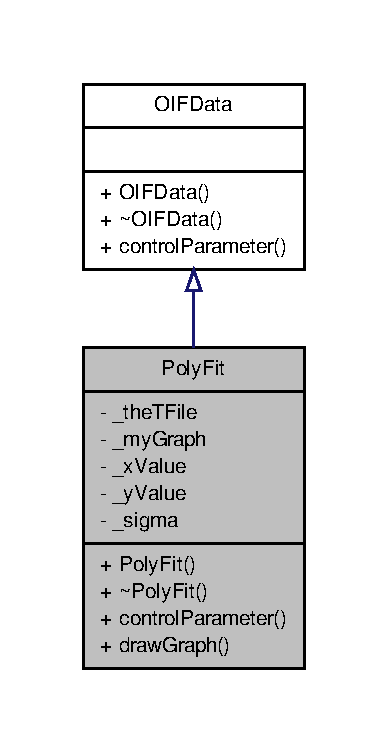
\includegraphics[width=186pt]{da/d58/classPolyFit__inherit__graph}
\end{center}
\end{figure}


Collaboration diagram for PolyFit:\nopagebreak
\begin{figure}[H]
\begin{center}
\leavevmode
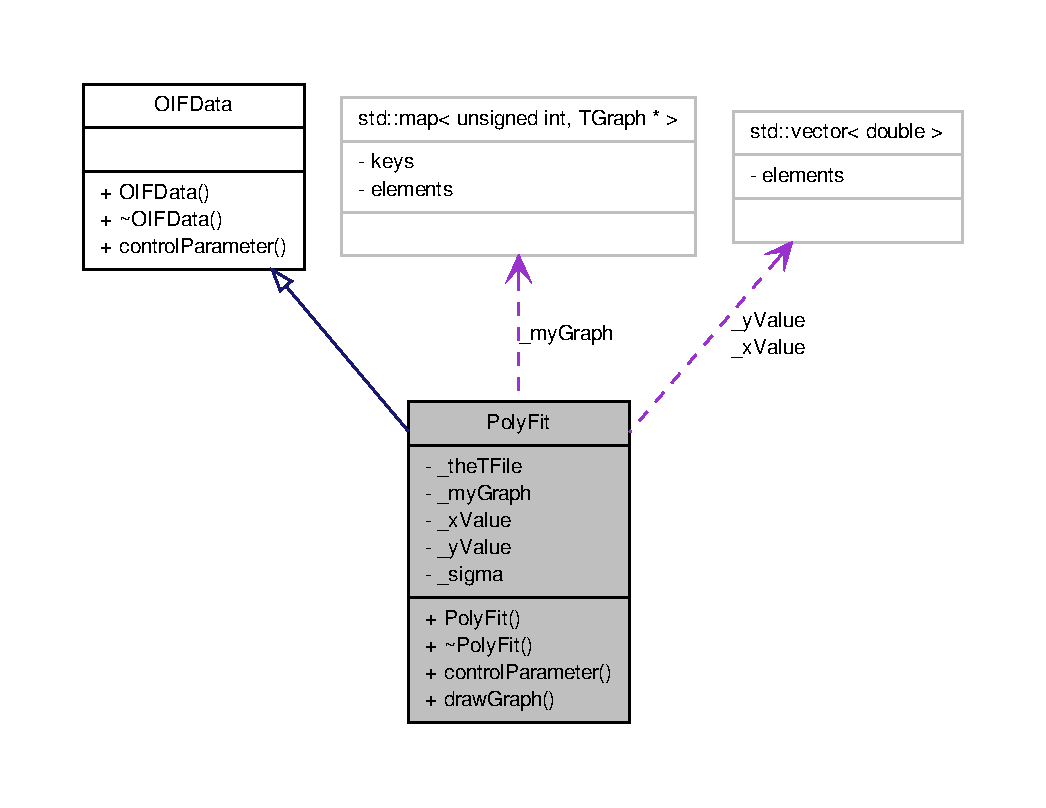
\includegraphics[width=400pt]{d6/d22/classPolyFit__coll__graph}
\end{center}
\end{figure}
\subsection*{Public Member Functions}
\begin{DoxyCompactItemize}
\item 
\hyperlink{classPolyFit_abfc9528462669ea53ce08e4945c4ce99}{PolyFit} (double p0, double p1, double p2, double p3, double sigma)
\begin{DoxyCompactList}\small\item\em Constructor. \end{DoxyCompactList}\item 
virtual \hyperlink{classPolyFit_a3462736e02f02d3ab46ccd64aaf235d3}{$\sim$PolyFit} ()
\item 
double \hyperlink{classPolyFit_a2f8bf8460f31aef010e67950c3db0c82}{controlParameter} (const vector$<$ \hyperlink{classPWAParameter}{PWAParameter}$<$ double $>$ $>$ \&minPar)
\item 
void \hyperlink{classPolyFit_ad90dd471fea18051d5c0c2e5b483f0a5}{drawGraph} (double a, double b, double c, double d)
\end{DoxyCompactItemize}
\subsection*{Private Attributes}
\begin{DoxyCompactItemize}
\item 
shared\_\-ptr$<$ TFile $>$ \hyperlink{classPolyFit_a9905a65c08ba059c98a0e4cf14dc1752}{\_\-theTFile}
\item 
map$<$ unsigned int, TGraph $\ast$ $>$ \hyperlink{classPolyFit_ae3de4c7d4cda8ce2cf162d9d70631cba}{\_\-myGraph}
\item 
vector$<$ double $>$ \hyperlink{classPolyFit_a0092a72e38616b0541f5ca2d3e109397}{\_\-xValue}
\item 
vector$<$ double $>$ \hyperlink{classPolyFit_a29d10890ebfda2ec6f0e7697dca5258f}{\_\-yValue}
\item 
double \hyperlink{classPolyFit_a0a19ea869319d65f97de4d0bc95e8061}{\_\-sigma}
\end{DoxyCompactItemize}


\subsection{Detailed Description}
Test implementation of \hyperlink{OIFData_8hpp}{OIFData.hpp}. 

\subsection{Constructor \& Destructor Documentation}
\hypertarget{classPolyFit_abfc9528462669ea53ce08e4945c4ce99}{
\index{PolyFit@{PolyFit}!PolyFit@{PolyFit}}
\index{PolyFit@{PolyFit}!PolyFit@{PolyFit}}
\subsubsection[{PolyFit}]{\setlength{\rightskip}{0pt plus 5cm}PolyFit::PolyFit (
\begin{DoxyParamCaption}
\item[{double}]{p0, }
\item[{double}]{p1, }
\item[{double}]{p2, }
\item[{double}]{p3, }
\item[{double}]{sigma}
\end{DoxyParamCaption}
)}}
\label{de/d89/classPolyFit_abfc9528462669ea53ce08e4945c4ce99}


Constructor. 

\hypertarget{classPolyFit_a3462736e02f02d3ab46ccd64aaf235d3}{
\index{PolyFit@{PolyFit}!$\sim$PolyFit@{$\sim$PolyFit}}
\index{$\sim$PolyFit@{$\sim$PolyFit}!PolyFit@{PolyFit}}
\subsubsection[{$\sim$PolyFit}]{\setlength{\rightskip}{0pt plus 5cm}PolyFit::$\sim$PolyFit (
\begin{DoxyParamCaption}
{}
\end{DoxyParamCaption}
)\hspace{0.3cm}{\ttfamily  \mbox{[}virtual\mbox{]}}}}
\label{de/d89/classPolyFit_a3462736e02f02d3ab46ccd64aaf235d3}
Destructor 

\subsection{Member Function Documentation}
\hypertarget{classPolyFit_a2f8bf8460f31aef010e67950c3db0c82}{
\index{PolyFit@{PolyFit}!controlParameter@{controlParameter}}
\index{controlParameter@{controlParameter}!PolyFit@{PolyFit}}
\subsubsection[{controlParameter}]{\setlength{\rightskip}{0pt plus 5cm}double PolyFit::controlParameter (
\begin{DoxyParamCaption}
\item[{const vector$<$ {\bf PWAParameter}$<$ double $>$ $>$ \&}]{minPar}
\end{DoxyParamCaption}
)\hspace{0.3cm}{\ttfamily  \mbox{[}virtual\mbox{]}}}}
\label{de/d89/classPolyFit_a2f8bf8460f31aef010e67950c3db0c82}


Implements \hyperlink{classOIFData_a12eef51d074a73b5b261c411e79cbb37}{OIFData}.

\hypertarget{classPolyFit_ad90dd471fea18051d5c0c2e5b483f0a5}{
\index{PolyFit@{PolyFit}!drawGraph@{drawGraph}}
\index{drawGraph@{drawGraph}!PolyFit@{PolyFit}}
\subsubsection[{drawGraph}]{\setlength{\rightskip}{0pt plus 5cm}void PolyFit::drawGraph (
\begin{DoxyParamCaption}
\item[{double}]{a, }
\item[{double}]{b, }
\item[{double}]{c, }
\item[{double}]{d}
\end{DoxyParamCaption}
)}}
\label{de/d89/classPolyFit_ad90dd471fea18051d5c0c2e5b483f0a5}


\subsection{Member Data Documentation}
\hypertarget{classPolyFit_ae3de4c7d4cda8ce2cf162d9d70631cba}{
\index{PolyFit@{PolyFit}!\_\-myGraph@{\_\-myGraph}}
\index{\_\-myGraph@{\_\-myGraph}!PolyFit@{PolyFit}}
\subsubsection[{\_\-myGraph}]{\setlength{\rightskip}{0pt plus 5cm}map$<$unsigned int, TGraph$\ast$ $>$ {\bf PolyFit::\_\-myGraph}\hspace{0.3cm}{\ttfamily  \mbox{[}private\mbox{]}}}}
\label{de/d89/classPolyFit_ae3de4c7d4cda8ce2cf162d9d70631cba}
\hypertarget{classPolyFit_a0a19ea869319d65f97de4d0bc95e8061}{
\index{PolyFit@{PolyFit}!\_\-sigma@{\_\-sigma}}
\index{\_\-sigma@{\_\-sigma}!PolyFit@{PolyFit}}
\subsubsection[{\_\-sigma}]{\setlength{\rightskip}{0pt plus 5cm}double {\bf PolyFit::\_\-sigma}\hspace{0.3cm}{\ttfamily  \mbox{[}private\mbox{]}}}}
\label{de/d89/classPolyFit_a0a19ea869319d65f97de4d0bc95e8061}
\hypertarget{classPolyFit_a9905a65c08ba059c98a0e4cf14dc1752}{
\index{PolyFit@{PolyFit}!\_\-theTFile@{\_\-theTFile}}
\index{\_\-theTFile@{\_\-theTFile}!PolyFit@{PolyFit}}
\subsubsection[{\_\-theTFile}]{\setlength{\rightskip}{0pt plus 5cm}shared\_\-ptr$<$TFile$>$ {\bf PolyFit::\_\-theTFile}\hspace{0.3cm}{\ttfamily  \mbox{[}private\mbox{]}}}}
\label{de/d89/classPolyFit_a9905a65c08ba059c98a0e4cf14dc1752}
\hypertarget{classPolyFit_a0092a72e38616b0541f5ca2d3e109397}{
\index{PolyFit@{PolyFit}!\_\-xValue@{\_\-xValue}}
\index{\_\-xValue@{\_\-xValue}!PolyFit@{PolyFit}}
\subsubsection[{\_\-xValue}]{\setlength{\rightskip}{0pt plus 5cm}vector$<$ double $>$ {\bf PolyFit::\_\-xValue}\hspace{0.3cm}{\ttfamily  \mbox{[}private\mbox{]}}}}
\label{de/d89/classPolyFit_a0092a72e38616b0541f5ca2d3e109397}
\hypertarget{classPolyFit_a29d10890ebfda2ec6f0e7697dca5258f}{
\index{PolyFit@{PolyFit}!\_\-yValue@{\_\-yValue}}
\index{\_\-yValue@{\_\-yValue}!PolyFit@{PolyFit}}
\subsubsection[{\_\-yValue}]{\setlength{\rightskip}{0pt plus 5cm}vector$<$ double $>$ {\bf PolyFit::\_\-yValue}\hspace{0.3cm}{\ttfamily  \mbox{[}private\mbox{]}}}}
\label{de/d89/classPolyFit_a29d10890ebfda2ec6f0e7697dca5258f}


The documentation for this class was generated from the following files:\begin{DoxyCompactItemize}
\item 
test/\hyperlink{PolyFit_8hpp}{PolyFit.hpp}\item 
test/\hyperlink{PolyFit_8cpp}{PolyFit.cpp}\end{DoxyCompactItemize}

\hypertarget{classPWAEvent}{
\section{PWAEvent Class Reference}
\label{dc/d66/classPWAEvent}\index{PWAEvent@{PWAEvent}}
}


Internal container for event information.  




{\ttfamily \#include $<$PWAEvent.hpp$>$}



Collaboration diagram for PWAEvent:\nopagebreak
\begin{figure}[H]
\begin{center}
\leavevmode
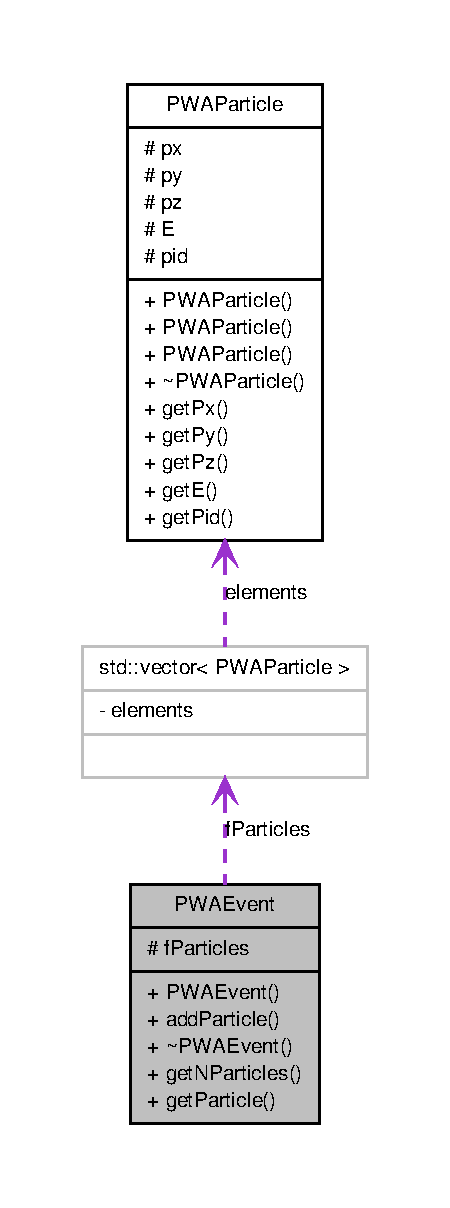
\includegraphics[width=216pt]{de/def/classPWAEvent__coll__graph}
\end{center}
\end{figure}
\subsection*{Public Member Functions}
\begin{DoxyCompactItemize}
\item 
\hyperlink{classPWAEvent_ad3c985fe0c67d2294ff58b99fb06a043}{PWAEvent} ()
\item 
virtual void \hyperlink{classPWAEvent_a9bacf043ab4eb9bff4e7b44580292d51}{addParticle} (\hyperlink{classPWAParticle}{PWAParticle} inParticle)
\item 
virtual \hyperlink{classPWAEvent_aed26fd206a7074baca66e27b3b983e55}{$\sim$PWAEvent} ()
\item 
virtual const unsigned int \hyperlink{classPWAEvent_a49b9731f3e38c7535c14bb0df3b032fc}{getNParticles} ()
\item 
virtual const int \hyperlink{classPWAEvent_a10ce3fc05ac0f64ac411b03a4d0f0138}{getParticle} (const unsigned int id, \hyperlink{classPWAParticle}{PWAParticle} \&out)
\end{DoxyCompactItemize}
\subsection*{Protected Attributes}
\begin{DoxyCompactItemize}
\item 
std::vector$<$ \hyperlink{classPWAParticle}{PWAParticle} $>$ \hyperlink{classPWAEvent_aac928bac7991d55225c0219c4c9ddf7a}{fParticles}
\end{DoxyCompactItemize}


\subsection{Detailed Description}
Internal container for event information. 

\subsection{Constructor \& Destructor Documentation}
\hypertarget{classPWAEvent_ad3c985fe0c67d2294ff58b99fb06a043}{
\index{PWAEvent@{PWAEvent}!PWAEvent@{PWAEvent}}
\index{PWAEvent@{PWAEvent}!PWAEvent@{PWAEvent}}
\subsubsection[{PWAEvent}]{\setlength{\rightskip}{0pt plus 5cm}PWAEvent::PWAEvent (
\begin{DoxyParamCaption}
{}
\end{DoxyParamCaption}
)}}
\label{dc/d66/classPWAEvent_ad3c985fe0c67d2294ff58b99fb06a043}
\hypertarget{classPWAEvent_aed26fd206a7074baca66e27b3b983e55}{
\index{PWAEvent@{PWAEvent}!$\sim$PWAEvent@{$\sim$PWAEvent}}
\index{$\sim$PWAEvent@{$\sim$PWAEvent}!PWAEvent@{PWAEvent}}
\subsubsection[{$\sim$PWAEvent}]{\setlength{\rightskip}{0pt plus 5cm}PWAEvent::$\sim$PWAEvent (
\begin{DoxyParamCaption}
{}
\end{DoxyParamCaption}
)\hspace{0.3cm}{\ttfamily  \mbox{[}virtual\mbox{]}}}}
\label{dc/d66/classPWAEvent_aed26fd206a7074baca66e27b3b983e55}


\subsection{Member Function Documentation}
\hypertarget{classPWAEvent_a9bacf043ab4eb9bff4e7b44580292d51}{
\index{PWAEvent@{PWAEvent}!addParticle@{addParticle}}
\index{addParticle@{addParticle}!PWAEvent@{PWAEvent}}
\subsubsection[{addParticle}]{\setlength{\rightskip}{0pt plus 5cm}void PWAEvent::addParticle (
\begin{DoxyParamCaption}
\item[{{\bf PWAParticle}}]{inParticle}
\end{DoxyParamCaption}
)\hspace{0.3cm}{\ttfamily  \mbox{[}virtual\mbox{]}}}}
\label{dc/d66/classPWAEvent_a9bacf043ab4eb9bff4e7b44580292d51}
\hypertarget{classPWAEvent_a49b9731f3e38c7535c14bb0df3b032fc}{
\index{PWAEvent@{PWAEvent}!getNParticles@{getNParticles}}
\index{getNParticles@{getNParticles}!PWAEvent@{PWAEvent}}
\subsubsection[{getNParticles}]{\setlength{\rightskip}{0pt plus 5cm}virtual const unsigned int PWAEvent::getNParticles (
\begin{DoxyParamCaption}
{}
\end{DoxyParamCaption}
)\hspace{0.3cm}{\ttfamily  \mbox{[}inline, virtual\mbox{]}}}}
\label{dc/d66/classPWAEvent_a49b9731f3e38c7535c14bb0df3b032fc}
\hypertarget{classPWAEvent_a10ce3fc05ac0f64ac411b03a4d0f0138}{
\index{PWAEvent@{PWAEvent}!getParticle@{getParticle}}
\index{getParticle@{getParticle}!PWAEvent@{PWAEvent}}
\subsubsection[{getParticle}]{\setlength{\rightskip}{0pt plus 5cm}const int PWAEvent::getParticle (
\begin{DoxyParamCaption}
\item[{const unsigned int}]{id, }
\item[{{\bf PWAParticle} \&}]{out}
\end{DoxyParamCaption}
)\hspace{0.3cm}{\ttfamily  \mbox{[}virtual\mbox{]}}}}
\label{dc/d66/classPWAEvent_a10ce3fc05ac0f64ac411b03a4d0f0138}


\subsection{Member Data Documentation}
\hypertarget{classPWAEvent_aac928bac7991d55225c0219c4c9ddf7a}{
\index{PWAEvent@{PWAEvent}!fParticles@{fParticles}}
\index{fParticles@{fParticles}!PWAEvent@{PWAEvent}}
\subsubsection[{fParticles}]{\setlength{\rightskip}{0pt plus 5cm}std::vector$<${\bf PWAParticle}$>$ {\bf PWAEvent::fParticles}\hspace{0.3cm}{\ttfamily  \mbox{[}protected\mbox{]}}}}
\label{dc/d66/classPWAEvent_aac928bac7991d55225c0219c4c9ddf7a}


The documentation for this class was generated from the following files:\begin{DoxyCompactItemize}
\item 
Core/\hyperlink{PWAEvent_8hpp}{PWAEvent.hpp}\item 
Core/\hyperlink{PWAEvent_8cpp}{PWAEvent.cpp}\end{DoxyCompactItemize}

\hypertarget{classPWAParameter}{
\section{PWAParameter$<$ T $>$ Class Template Reference}
\label{d2/d41/classPWAParameter}\index{PWAParameter@{PWAParameter}}
}


Internal container representing a parameter.  




{\ttfamily \#include $<$PWAParameter.hpp$>$}



Collaboration diagram for PWAParameter$<$ T $>$:\nopagebreak
\begin{figure}[H]
\begin{center}
\leavevmode
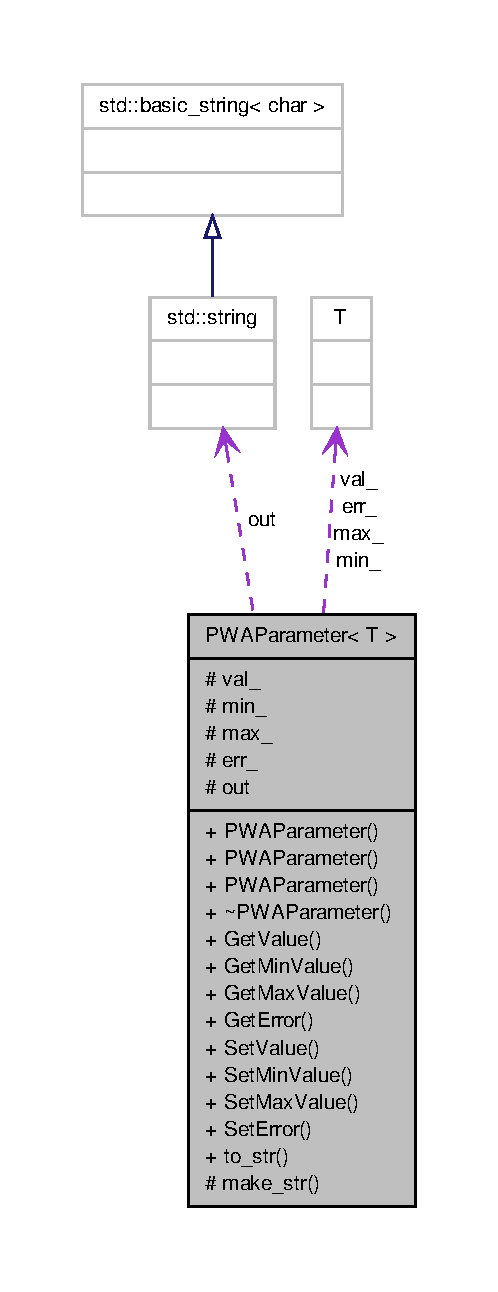
\includegraphics[height=600pt]{de/d75/classPWAParameter__coll__graph}
\end{center}
\end{figure}
\subsection*{Public Member Functions}
\begin{DoxyCompactItemize}
\item 
\hyperlink{classPWAParameter_a4be4f99ee7b087966625af22b6724d2b}{PWAParameter} ()
\item 
\hyperlink{classPWAParameter_a1fd9d62e6e6d9665fa8f50a01ea44e08}{PWAParameter} (const T value, const T min, const T max, const T error)
\item 
\hyperlink{classPWAParameter_a26d29b6f5db20ce28bffb4f8f51f103d}{PWAParameter} (const \hyperlink{classPWAParameter}{PWAParameter}$<$ T $>$ \&in)
\item 
virtual \hyperlink{classPWAParameter_abe9cf9e35dd365263bab2ba448417320}{$\sim$PWAParameter} ()
\item 
virtual const T \hyperlink{classPWAParameter_aeb63b119db2a408ba1a69b057458e476}{GetValue} () const 
\item 
virtual const T \hyperlink{classPWAParameter_ad56bff0ec385ebc123f980fd932b7679}{GetMinValue} () const 
\item 
virtual const T \hyperlink{classPWAParameter_ae2cf7ce619f8539dd2d54fb836fc6881}{GetMaxValue} () const 
\item 
virtual const T \hyperlink{classPWAParameter_afa71b91326c07eadcc832928d21fcc1c}{GetError} () const 
\item 
virtual void \hyperlink{classPWAParameter_a5b0aeb09e7f770c8196d5afc08f59320}{SetValue} (const T value)
\item 
virtual void \hyperlink{classPWAParameter_abd0ed2ea7347c9a74eb2f9f1a0871198}{SetMinValue} (const T min)
\item 
virtual void \hyperlink{classPWAParameter_a2681d68a47e40c4226e7eee63dca985a}{SetMaxValue} (const T max)
\item 
virtual void \hyperlink{classPWAParameter_add37911ceeaddfaa2e4b8a2ce7ca5947}{SetError} (const T error)
\item 
std::string const \& \hyperlink{classPWAParameter_aaea7aaa18a729118f0fcb75ef2fdbb8c}{to\_\-str} () const 
\end{DoxyCompactItemize}
\subsection*{Protected Member Functions}
\begin{DoxyCompactItemize}
\item 
void \hyperlink{classPWAParameter_ad61ee62933b2b6b8edf73efde8e8e71b}{make\_\-str} ()
\end{DoxyCompactItemize}
\subsection*{Protected Attributes}
\begin{DoxyCompactItemize}
\item 
T \hyperlink{classPWAParameter_a340ff1428a7859762b83ee9f607b45b5}{val\_\-}
\item 
T \hyperlink{classPWAParameter_aafd4f577aa33a901f7ed8e7544158af0}{min\_\-}
\item 
T \hyperlink{classPWAParameter_a6baf4acd771fc311860d1f8c5ff01026}{max\_\-}
\item 
T \hyperlink{classPWAParameter_acea642e8ce9666a54bcecffc573acbde}{err\_\-}
\item 
std::string \hyperlink{classPWAParameter_aa2b305c00ce772a886f23cabe1170a08}{out}
\end{DoxyCompactItemize}
\subsection*{Friends}
\begin{DoxyCompactItemize}
\item 
{\footnotesize template$<$class U $>$ }\\std::ostream \& \hyperlink{classPWAParameter_a22f81859f3803c4acbd53ccf03d50780}{operator$<$$<$} (std::ostream \&os, const \hyperlink{classPWAParameter}{PWAParameter}$<$ U $>$ \&p)
\end{DoxyCompactItemize}


\subsection{Detailed Description}
\subsubsection*{template$<$class T$>$class PWAParameter$<$ T $>$}

Internal container representing a parameter. 

\subsection{Constructor \& Destructor Documentation}
\hypertarget{classPWAParameter_a4be4f99ee7b087966625af22b6724d2b}{
\index{PWAParameter@{PWAParameter}!PWAParameter@{PWAParameter}}
\index{PWAParameter@{PWAParameter}!PWAParameter@{PWAParameter}}
\subsubsection[{PWAParameter}]{\setlength{\rightskip}{0pt plus 5cm}template$<$class T$>$ {\bf PWAParameter}$<$ T $>$::{\bf PWAParameter} (
\begin{DoxyParamCaption}
{}
\end{DoxyParamCaption}
)\hspace{0.3cm}{\ttfamily  \mbox{[}inline\mbox{]}}}}
\label{d2/d41/classPWAParameter_a4be4f99ee7b087966625af22b6724d2b}
\hypertarget{classPWAParameter_a1fd9d62e6e6d9665fa8f50a01ea44e08}{
\index{PWAParameter@{PWAParameter}!PWAParameter@{PWAParameter}}
\index{PWAParameter@{PWAParameter}!PWAParameter@{PWAParameter}}
\subsubsection[{PWAParameter}]{\setlength{\rightskip}{0pt plus 5cm}template$<$class T$>$ {\bf PWAParameter}$<$ T $>$::{\bf PWAParameter} (
\begin{DoxyParamCaption}
\item[{const T}]{value, }
\item[{const T}]{min, }
\item[{const T}]{max, }
\item[{const T}]{error}
\end{DoxyParamCaption}
)\hspace{0.3cm}{\ttfamily  \mbox{[}inline\mbox{]}}}}
\label{d2/d41/classPWAParameter_a1fd9d62e6e6d9665fa8f50a01ea44e08}
\hypertarget{classPWAParameter_a26d29b6f5db20ce28bffb4f8f51f103d}{
\index{PWAParameter@{PWAParameter}!PWAParameter@{PWAParameter}}
\index{PWAParameter@{PWAParameter}!PWAParameter@{PWAParameter}}
\subsubsection[{PWAParameter}]{\setlength{\rightskip}{0pt plus 5cm}template$<$class T$>$ {\bf PWAParameter}$<$ T $>$::{\bf PWAParameter} (
\begin{DoxyParamCaption}
\item[{const {\bf PWAParameter}$<$ T $>$ \&}]{in}
\end{DoxyParamCaption}
)\hspace{0.3cm}{\ttfamily  \mbox{[}inline\mbox{]}}}}
\label{d2/d41/classPWAParameter_a26d29b6f5db20ce28bffb4f8f51f103d}
\hypertarget{classPWAParameter_abe9cf9e35dd365263bab2ba448417320}{
\index{PWAParameter@{PWAParameter}!$\sim$PWAParameter@{$\sim$PWAParameter}}
\index{$\sim$PWAParameter@{$\sim$PWAParameter}!PWAParameter@{PWAParameter}}
\subsubsection[{$\sim$PWAParameter}]{\setlength{\rightskip}{0pt plus 5cm}template$<$class T$>$ virtual {\bf PWAParameter}$<$ T $>$::$\sim${\bf PWAParameter} (
\begin{DoxyParamCaption}
{}
\end{DoxyParamCaption}
)\hspace{0.3cm}{\ttfamily  \mbox{[}inline, virtual\mbox{]}}}}
\label{d2/d41/classPWAParameter_abe9cf9e35dd365263bab2ba448417320}


\subsection{Member Function Documentation}
\hypertarget{classPWAParameter_afa71b91326c07eadcc832928d21fcc1c}{
\index{PWAParameter@{PWAParameter}!GetError@{GetError}}
\index{GetError@{GetError}!PWAParameter@{PWAParameter}}
\subsubsection[{GetError}]{\setlength{\rightskip}{0pt plus 5cm}template$<$class T$>$ virtual const T {\bf PWAParameter}$<$ T $>$::GetError (
\begin{DoxyParamCaption}
{}
\end{DoxyParamCaption}
) const\hspace{0.3cm}{\ttfamily  \mbox{[}inline, virtual\mbox{]}}}}
\label{d2/d41/classPWAParameter_afa71b91326c07eadcc832928d21fcc1c}
\hypertarget{classPWAParameter_ae2cf7ce619f8539dd2d54fb836fc6881}{
\index{PWAParameter@{PWAParameter}!GetMaxValue@{GetMaxValue}}
\index{GetMaxValue@{GetMaxValue}!PWAParameter@{PWAParameter}}
\subsubsection[{GetMaxValue}]{\setlength{\rightskip}{0pt plus 5cm}template$<$class T$>$ virtual const T {\bf PWAParameter}$<$ T $>$::GetMaxValue (
\begin{DoxyParamCaption}
{}
\end{DoxyParamCaption}
) const\hspace{0.3cm}{\ttfamily  \mbox{[}inline, virtual\mbox{]}}}}
\label{d2/d41/classPWAParameter_ae2cf7ce619f8539dd2d54fb836fc6881}
\hypertarget{classPWAParameter_ad56bff0ec385ebc123f980fd932b7679}{
\index{PWAParameter@{PWAParameter}!GetMinValue@{GetMinValue}}
\index{GetMinValue@{GetMinValue}!PWAParameter@{PWAParameter}}
\subsubsection[{GetMinValue}]{\setlength{\rightskip}{0pt plus 5cm}template$<$class T$>$ virtual const T {\bf PWAParameter}$<$ T $>$::GetMinValue (
\begin{DoxyParamCaption}
{}
\end{DoxyParamCaption}
) const\hspace{0.3cm}{\ttfamily  \mbox{[}inline, virtual\mbox{]}}}}
\label{d2/d41/classPWAParameter_ad56bff0ec385ebc123f980fd932b7679}
\hypertarget{classPWAParameter_aeb63b119db2a408ba1a69b057458e476}{
\index{PWAParameter@{PWAParameter}!GetValue@{GetValue}}
\index{GetValue@{GetValue}!PWAParameter@{PWAParameter}}
\subsubsection[{GetValue}]{\setlength{\rightskip}{0pt plus 5cm}template$<$class T$>$ virtual const T {\bf PWAParameter}$<$ T $>$::GetValue (
\begin{DoxyParamCaption}
{}
\end{DoxyParamCaption}
) const\hspace{0.3cm}{\ttfamily  \mbox{[}inline, virtual\mbox{]}}}}
\label{d2/d41/classPWAParameter_aeb63b119db2a408ba1a69b057458e476}
\hypertarget{classPWAParameter_ad61ee62933b2b6b8edf73efde8e8e71b}{
\index{PWAParameter@{PWAParameter}!make\_\-str@{make\_\-str}}
\index{make\_\-str@{make\_\-str}!PWAParameter@{PWAParameter}}
\subsubsection[{make\_\-str}]{\setlength{\rightskip}{0pt plus 5cm}template$<$class T$>$ void {\bf PWAParameter}$<$ T $>$::make\_\-str (
\begin{DoxyParamCaption}
{}
\end{DoxyParamCaption}
)\hspace{0.3cm}{\ttfamily  \mbox{[}inline, protected\mbox{]}}}}
\label{d2/d41/classPWAParameter_ad61ee62933b2b6b8edf73efde8e8e71b}
\hypertarget{classPWAParameter_add37911ceeaddfaa2e4b8a2ce7ca5947}{
\index{PWAParameter@{PWAParameter}!SetError@{SetError}}
\index{SetError@{SetError}!PWAParameter@{PWAParameter}}
\subsubsection[{SetError}]{\setlength{\rightskip}{0pt plus 5cm}template$<$class T$>$ virtual void {\bf PWAParameter}$<$ T $>$::SetError (
\begin{DoxyParamCaption}
\item[{const T}]{error}
\end{DoxyParamCaption}
)\hspace{0.3cm}{\ttfamily  \mbox{[}inline, virtual\mbox{]}}}}
\label{d2/d41/classPWAParameter_add37911ceeaddfaa2e4b8a2ce7ca5947}
\hypertarget{classPWAParameter_a2681d68a47e40c4226e7eee63dca985a}{
\index{PWAParameter@{PWAParameter}!SetMaxValue@{SetMaxValue}}
\index{SetMaxValue@{SetMaxValue}!PWAParameter@{PWAParameter}}
\subsubsection[{SetMaxValue}]{\setlength{\rightskip}{0pt plus 5cm}template$<$class T$>$ virtual void {\bf PWAParameter}$<$ T $>$::SetMaxValue (
\begin{DoxyParamCaption}
\item[{const T}]{max}
\end{DoxyParamCaption}
)\hspace{0.3cm}{\ttfamily  \mbox{[}inline, virtual\mbox{]}}}}
\label{d2/d41/classPWAParameter_a2681d68a47e40c4226e7eee63dca985a}
\hypertarget{classPWAParameter_abd0ed2ea7347c9a74eb2f9f1a0871198}{
\index{PWAParameter@{PWAParameter}!SetMinValue@{SetMinValue}}
\index{SetMinValue@{SetMinValue}!PWAParameter@{PWAParameter}}
\subsubsection[{SetMinValue}]{\setlength{\rightskip}{0pt plus 5cm}template$<$class T$>$ virtual void {\bf PWAParameter}$<$ T $>$::SetMinValue (
\begin{DoxyParamCaption}
\item[{const T}]{min}
\end{DoxyParamCaption}
)\hspace{0.3cm}{\ttfamily  \mbox{[}inline, virtual\mbox{]}}}}
\label{d2/d41/classPWAParameter_abd0ed2ea7347c9a74eb2f9f1a0871198}
\hypertarget{classPWAParameter_a5b0aeb09e7f770c8196d5afc08f59320}{
\index{PWAParameter@{PWAParameter}!SetValue@{SetValue}}
\index{SetValue@{SetValue}!PWAParameter@{PWAParameter}}
\subsubsection[{SetValue}]{\setlength{\rightskip}{0pt plus 5cm}template$<$class T$>$ virtual void {\bf PWAParameter}$<$ T $>$::SetValue (
\begin{DoxyParamCaption}
\item[{const T}]{value}
\end{DoxyParamCaption}
)\hspace{0.3cm}{\ttfamily  \mbox{[}inline, virtual\mbox{]}}}}
\label{d2/d41/classPWAParameter_a5b0aeb09e7f770c8196d5afc08f59320}
\hypertarget{classPWAParameter_aaea7aaa18a729118f0fcb75ef2fdbb8c}{
\index{PWAParameter@{PWAParameter}!to\_\-str@{to\_\-str}}
\index{to\_\-str@{to\_\-str}!PWAParameter@{PWAParameter}}
\subsubsection[{to\_\-str}]{\setlength{\rightskip}{0pt plus 5cm}template$<$class T$>$ std::string const\& {\bf PWAParameter}$<$ T $>$::to\_\-str (
\begin{DoxyParamCaption}
{}
\end{DoxyParamCaption}
) const\hspace{0.3cm}{\ttfamily  \mbox{[}inline\mbox{]}}}}
\label{d2/d41/classPWAParameter_aaea7aaa18a729118f0fcb75ef2fdbb8c}


\subsection{Friends And Related Function Documentation}
\hypertarget{classPWAParameter_a22f81859f3803c4acbd53ccf03d50780}{
\index{PWAParameter@{PWAParameter}!operator$<$$<$@{operator$<$$<$}}
\index{operator$<$$<$@{operator$<$$<$}!PWAParameter@{PWAParameter}}
\subsubsection[{operator$<$$<$}]{\setlength{\rightskip}{0pt plus 5cm}template$<$class T$>$ template$<$class U $>$ std::ostream\& operator$<$$<$ (
\begin{DoxyParamCaption}
\item[{std::ostream \&}]{os, }
\item[{const {\bf PWAParameter}$<$ U $>$ \&}]{p}
\end{DoxyParamCaption}
)\hspace{0.3cm}{\ttfamily  \mbox{[}friend\mbox{]}}}}
\label{d2/d41/classPWAParameter_a22f81859f3803c4acbd53ccf03d50780}


\subsection{Member Data Documentation}
\hypertarget{classPWAParameter_acea642e8ce9666a54bcecffc573acbde}{
\index{PWAParameter@{PWAParameter}!err\_\-@{err\_\-}}
\index{err\_\-@{err\_\-}!PWAParameter@{PWAParameter}}
\subsubsection[{err\_\-}]{\setlength{\rightskip}{0pt plus 5cm}template$<$class T$>$ T {\bf PWAParameter}$<$ T $>$::{\bf err\_\-}\hspace{0.3cm}{\ttfamily  \mbox{[}protected\mbox{]}}}}
\label{d2/d41/classPWAParameter_acea642e8ce9666a54bcecffc573acbde}
\hypertarget{classPWAParameter_a6baf4acd771fc311860d1f8c5ff01026}{
\index{PWAParameter@{PWAParameter}!max\_\-@{max\_\-}}
\index{max\_\-@{max\_\-}!PWAParameter@{PWAParameter}}
\subsubsection[{max\_\-}]{\setlength{\rightskip}{0pt plus 5cm}template$<$class T$>$ T {\bf PWAParameter}$<$ T $>$::{\bf max\_\-}\hspace{0.3cm}{\ttfamily  \mbox{[}protected\mbox{]}}}}
\label{d2/d41/classPWAParameter_a6baf4acd771fc311860d1f8c5ff01026}
\hypertarget{classPWAParameter_aafd4f577aa33a901f7ed8e7544158af0}{
\index{PWAParameter@{PWAParameter}!min\_\-@{min\_\-}}
\index{min\_\-@{min\_\-}!PWAParameter@{PWAParameter}}
\subsubsection[{min\_\-}]{\setlength{\rightskip}{0pt plus 5cm}template$<$class T$>$ T {\bf PWAParameter}$<$ T $>$::{\bf min\_\-}\hspace{0.3cm}{\ttfamily  \mbox{[}protected\mbox{]}}}}
\label{d2/d41/classPWAParameter_aafd4f577aa33a901f7ed8e7544158af0}
\hypertarget{classPWAParameter_aa2b305c00ce772a886f23cabe1170a08}{
\index{PWAParameter@{PWAParameter}!out@{out}}
\index{out@{out}!PWAParameter@{PWAParameter}}
\subsubsection[{out}]{\setlength{\rightskip}{0pt plus 5cm}template$<$class T$>$ std::string {\bf PWAParameter}$<$ T $>$::{\bf out}\hspace{0.3cm}{\ttfamily  \mbox{[}protected\mbox{]}}}}
\label{d2/d41/classPWAParameter_aa2b305c00ce772a886f23cabe1170a08}
\hypertarget{classPWAParameter_a340ff1428a7859762b83ee9f607b45b5}{
\index{PWAParameter@{PWAParameter}!val\_\-@{val\_\-}}
\index{val\_\-@{val\_\-}!PWAParameter@{PWAParameter}}
\subsubsection[{val\_\-}]{\setlength{\rightskip}{0pt plus 5cm}template$<$class T$>$ T {\bf PWAParameter}$<$ T $>$::{\bf val\_\-}\hspace{0.3cm}{\ttfamily  \mbox{[}protected\mbox{]}}}}
\label{d2/d41/classPWAParameter_a340ff1428a7859762b83ee9f607b45b5}


The documentation for this class was generated from the following file:\begin{DoxyCompactItemize}
\item 
Core/\hyperlink{PWAParameter_8hpp}{PWAParameter.hpp}\end{DoxyCompactItemize}

\hypertarget{classPWAParticle}{
\section{PWAParticle Class Reference}
\label{d9/dcb/classPWAParticle}\index{PWAParticle@{PWAParticle}}
}


Internal container representing a particle.  




{\ttfamily \#include $<$PWAParticle.hpp$>$}

\subsection*{Public Member Functions}
\begin{DoxyCompactItemize}
\item 
\hyperlink{classPWAParticle_ad2757e82d6f72eb190f2a5530f5873d3}{PWAParticle} ()
\item 
\hyperlink{classPWAParticle_a05dccc6d5ab7b646a08970cd170afcd5}{PWAParticle} (double inPx, double inPy, double inPz, double inE, int inpid=0)
\item 
\hyperlink{classPWAParticle_a0d440b263ef67cbfca30cbed4c8d3bb0}{PWAParticle} (const \hyperlink{classPWAParticle}{PWAParticle} \&inParticle)
\item 
virtual \hyperlink{classPWAParticle_af90e6b356ab1069a0f3aa09b6b1be95e}{$\sim$PWAParticle} ()
\item 
virtual const double \hyperlink{classPWAParticle_a983609ee7bb185843079a9efc34224ec}{getPx} () const 
\item 
virtual const double \hyperlink{classPWAParticle_aadee7eda584f3efb78ed942f3bf02f46}{getPy} () const 
\item 
virtual const double \hyperlink{classPWAParticle_af367d5bac6dc8995d071b4435da8de9c}{getPz} () const 
\item 
virtual const double \hyperlink{classPWAParticle_a1b4990b52e0a4de681e1192645c60d53}{getE} () const 
\item 
virtual const int \hyperlink{classPWAParticle_a0ae39e4858d572a07bd0fac1de0c2d31}{getPid} () const 
\end{DoxyCompactItemize}
\subsection*{Protected Attributes}
\begin{DoxyCompactItemize}
\item 
double \hyperlink{classPWAParticle_a785b498941ebc062698dbd34be8c6d96}{px}
\item 
double \hyperlink{classPWAParticle_a51a443171d65b2abd885c51f92068f85}{py}
\item 
double \hyperlink{classPWAParticle_aaf5605fd8e557449072e9437add86a15}{pz}
\item 
double \hyperlink{classPWAParticle_ae1b3e03ff18925509275e763e3a76417}{E}
\item 
int \hyperlink{classPWAParticle_af45a7569c8ddbf0b8971cbbc24ab879d}{pid}
\end{DoxyCompactItemize}


\subsection{Detailed Description}
Internal container representing a particle. 

\subsection{Constructor \& Destructor Documentation}
\hypertarget{classPWAParticle_ad2757e82d6f72eb190f2a5530f5873d3}{
\index{PWAParticle@{PWAParticle}!PWAParticle@{PWAParticle}}
\index{PWAParticle@{PWAParticle}!PWAParticle@{PWAParticle}}
\subsubsection[{PWAParticle}]{\setlength{\rightskip}{0pt plus 5cm}PWAParticle::PWAParticle (
\begin{DoxyParamCaption}
{}
\end{DoxyParamCaption}
)\hspace{0.3cm}{\ttfamily  \mbox{[}inline\mbox{]}}}}
\label{d9/dcb/classPWAParticle_ad2757e82d6f72eb190f2a5530f5873d3}
\hypertarget{classPWAParticle_a05dccc6d5ab7b646a08970cd170afcd5}{
\index{PWAParticle@{PWAParticle}!PWAParticle@{PWAParticle}}
\index{PWAParticle@{PWAParticle}!PWAParticle@{PWAParticle}}
\subsubsection[{PWAParticle}]{\setlength{\rightskip}{0pt plus 5cm}PWAParticle::PWAParticle (
\begin{DoxyParamCaption}
\item[{double}]{inPx, }
\item[{double}]{inPy, }
\item[{double}]{inPz, }
\item[{double}]{inE, }
\item[{int}]{inpid = {\ttfamily 0}}
\end{DoxyParamCaption}
)\hspace{0.3cm}{\ttfamily  \mbox{[}inline\mbox{]}}}}
\label{d9/dcb/classPWAParticle_a05dccc6d5ab7b646a08970cd170afcd5}
\hypertarget{classPWAParticle_a0d440b263ef67cbfca30cbed4c8d3bb0}{
\index{PWAParticle@{PWAParticle}!PWAParticle@{PWAParticle}}
\index{PWAParticle@{PWAParticle}!PWAParticle@{PWAParticle}}
\subsubsection[{PWAParticle}]{\setlength{\rightskip}{0pt plus 5cm}PWAParticle::PWAParticle (
\begin{DoxyParamCaption}
\item[{const {\bf PWAParticle} \&}]{inParticle}
\end{DoxyParamCaption}
)\hspace{0.3cm}{\ttfamily  \mbox{[}inline\mbox{]}}}}
\label{d9/dcb/classPWAParticle_a0d440b263ef67cbfca30cbed4c8d3bb0}
\hypertarget{classPWAParticle_af90e6b356ab1069a0f3aa09b6b1be95e}{
\index{PWAParticle@{PWAParticle}!$\sim$PWAParticle@{$\sim$PWAParticle}}
\index{$\sim$PWAParticle@{$\sim$PWAParticle}!PWAParticle@{PWAParticle}}
\subsubsection[{$\sim$PWAParticle}]{\setlength{\rightskip}{0pt plus 5cm}virtual PWAParticle::$\sim$PWAParticle (
\begin{DoxyParamCaption}
{}
\end{DoxyParamCaption}
)\hspace{0.3cm}{\ttfamily  \mbox{[}inline, virtual\mbox{]}}}}
\label{d9/dcb/classPWAParticle_af90e6b356ab1069a0f3aa09b6b1be95e}


\subsection{Member Function Documentation}
\hypertarget{classPWAParticle_a1b4990b52e0a4de681e1192645c60d53}{
\index{PWAParticle@{PWAParticle}!getE@{getE}}
\index{getE@{getE}!PWAParticle@{PWAParticle}}
\subsubsection[{getE}]{\setlength{\rightskip}{0pt plus 5cm}virtual const double PWAParticle::getE (
\begin{DoxyParamCaption}
{}
\end{DoxyParamCaption}
) const\hspace{0.3cm}{\ttfamily  \mbox{[}inline, virtual\mbox{]}}}}
\label{d9/dcb/classPWAParticle_a1b4990b52e0a4de681e1192645c60d53}
\hypertarget{classPWAParticle_a0ae39e4858d572a07bd0fac1de0c2d31}{
\index{PWAParticle@{PWAParticle}!getPid@{getPid}}
\index{getPid@{getPid}!PWAParticle@{PWAParticle}}
\subsubsection[{getPid}]{\setlength{\rightskip}{0pt plus 5cm}virtual const int PWAParticle::getPid (
\begin{DoxyParamCaption}
{}
\end{DoxyParamCaption}
) const\hspace{0.3cm}{\ttfamily  \mbox{[}inline, virtual\mbox{]}}}}
\label{d9/dcb/classPWAParticle_a0ae39e4858d572a07bd0fac1de0c2d31}
\hypertarget{classPWAParticle_a983609ee7bb185843079a9efc34224ec}{
\index{PWAParticle@{PWAParticle}!getPx@{getPx}}
\index{getPx@{getPx}!PWAParticle@{PWAParticle}}
\subsubsection[{getPx}]{\setlength{\rightskip}{0pt plus 5cm}virtual const double PWAParticle::getPx (
\begin{DoxyParamCaption}
{}
\end{DoxyParamCaption}
) const\hspace{0.3cm}{\ttfamily  \mbox{[}inline, virtual\mbox{]}}}}
\label{d9/dcb/classPWAParticle_a983609ee7bb185843079a9efc34224ec}
\hypertarget{classPWAParticle_aadee7eda584f3efb78ed942f3bf02f46}{
\index{PWAParticle@{PWAParticle}!getPy@{getPy}}
\index{getPy@{getPy}!PWAParticle@{PWAParticle}}
\subsubsection[{getPy}]{\setlength{\rightskip}{0pt plus 5cm}virtual const double PWAParticle::getPy (
\begin{DoxyParamCaption}
{}
\end{DoxyParamCaption}
) const\hspace{0.3cm}{\ttfamily  \mbox{[}inline, virtual\mbox{]}}}}
\label{d9/dcb/classPWAParticle_aadee7eda584f3efb78ed942f3bf02f46}
\hypertarget{classPWAParticle_af367d5bac6dc8995d071b4435da8de9c}{
\index{PWAParticle@{PWAParticle}!getPz@{getPz}}
\index{getPz@{getPz}!PWAParticle@{PWAParticle}}
\subsubsection[{getPz}]{\setlength{\rightskip}{0pt plus 5cm}virtual const double PWAParticle::getPz (
\begin{DoxyParamCaption}
{}
\end{DoxyParamCaption}
) const\hspace{0.3cm}{\ttfamily  \mbox{[}inline, virtual\mbox{]}}}}
\label{d9/dcb/classPWAParticle_af367d5bac6dc8995d071b4435da8de9c}


\subsection{Member Data Documentation}
\hypertarget{classPWAParticle_ae1b3e03ff18925509275e763e3a76417}{
\index{PWAParticle@{PWAParticle}!E@{E}}
\index{E@{E}!PWAParticle@{PWAParticle}}
\subsubsection[{E}]{\setlength{\rightskip}{0pt plus 5cm}double {\bf PWAParticle::E}\hspace{0.3cm}{\ttfamily  \mbox{[}protected\mbox{]}}}}
\label{d9/dcb/classPWAParticle_ae1b3e03ff18925509275e763e3a76417}
\hypertarget{classPWAParticle_af45a7569c8ddbf0b8971cbbc24ab879d}{
\index{PWAParticle@{PWAParticle}!pid@{pid}}
\index{pid@{pid}!PWAParticle@{PWAParticle}}
\subsubsection[{pid}]{\setlength{\rightskip}{0pt plus 5cm}int {\bf PWAParticle::pid}\hspace{0.3cm}{\ttfamily  \mbox{[}protected\mbox{]}}}}
\label{d9/dcb/classPWAParticle_af45a7569c8ddbf0b8971cbbc24ab879d}
\hypertarget{classPWAParticle_a785b498941ebc062698dbd34be8c6d96}{
\index{PWAParticle@{PWAParticle}!px@{px}}
\index{px@{px}!PWAParticle@{PWAParticle}}
\subsubsection[{px}]{\setlength{\rightskip}{0pt plus 5cm}double {\bf PWAParticle::px}\hspace{0.3cm}{\ttfamily  \mbox{[}protected\mbox{]}}}}
\label{d9/dcb/classPWAParticle_a785b498941ebc062698dbd34be8c6d96}
\hypertarget{classPWAParticle_a51a443171d65b2abd885c51f92068f85}{
\index{PWAParticle@{PWAParticle}!py@{py}}
\index{py@{py}!PWAParticle@{PWAParticle}}
\subsubsection[{py}]{\setlength{\rightskip}{0pt plus 5cm}double {\bf PWAParticle::py}\hspace{0.3cm}{\ttfamily  \mbox{[}protected\mbox{]}}}}
\label{d9/dcb/classPWAParticle_a51a443171d65b2abd885c51f92068f85}
\hypertarget{classPWAParticle_aaf5605fd8e557449072e9437add86a15}{
\index{PWAParticle@{PWAParticle}!pz@{pz}}
\index{pz@{pz}!PWAParticle@{PWAParticle}}
\subsubsection[{pz}]{\setlength{\rightskip}{0pt plus 5cm}double {\bf PWAParticle::pz}\hspace{0.3cm}{\ttfamily  \mbox{[}protected\mbox{]}}}}
\label{d9/dcb/classPWAParticle_aaf5605fd8e557449072e9437add86a15}


The documentation for this class was generated from the following file:\begin{DoxyCompactItemize}
\item 
Core/\hyperlink{PWAParticle_8hpp}{PWAParticle.hpp}\end{DoxyCompactItemize}

\chapter{File Documentation}
\hypertarget{DIFBase_8hpp}{
\section{Core/DIFBase.hpp File Reference}
\label{db/d2c/DIFBase_8hpp}\index{Core/DIFBase.hpp@{Core/DIFBase.hpp}}
}


This class provides the interface to experimental data.  


{\ttfamily \#include \char`\"{}PWAEvent.hpp\char`\"{}}\par
Include dependency graph for DIFBase.hpp:\nopagebreak
\begin{figure}[H]
\begin{center}
\leavevmode
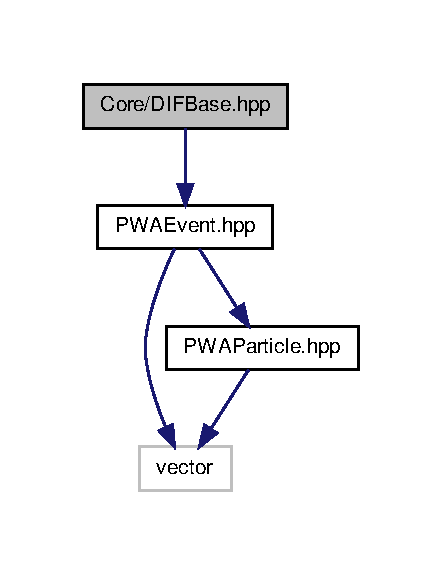
\includegraphics[width=212pt]{d7/d2a/DIFBase_8hpp__incl}
\end{center}
\end{figure}
This graph shows which files directly or indirectly include this file:
\nopagebreak
\begin{figure}[H]
\begin{center}
\leavevmode
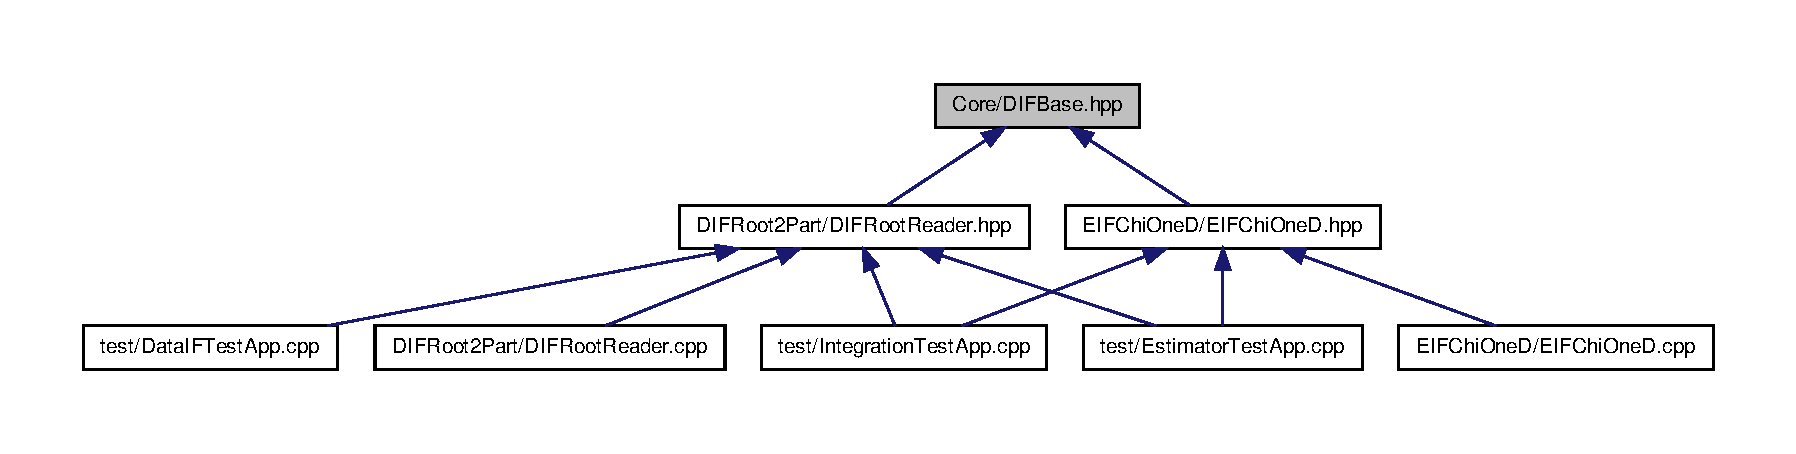
\includegraphics[width=400pt]{d8/d7d/DIFBase_8hpp__dep__incl}
\end{center}
\end{figure}
\subsection*{Classes}
\begin{DoxyCompactItemize}
\item 
class \hyperlink{classDIFBase}{DIFBase}
\begin{DoxyCompactList}\small\item\em Data Interface Base-\/Class. \end{DoxyCompactList}\end{DoxyCompactItemize}


\subsection{Detailed Description}
This class provides the interface to experimental data. As it is pure virtual, one needs at least one implementation to provide data for the other modules. If a new reader is derived from and fulfills this base-\/class, no change in other modules are necessary to work with the new dataset. 
\hypertarget{EIFBase_8hpp}{
\section{Core/EIFBase.hpp File Reference}
\label{df/d05/EIFBase_8hpp}\index{Core/EIFBase.hpp@{Core/EIFBase.hpp}}
}


This class provides the interface to classes which estimate the \char`\"{}closeness\char`\"{} of the modeled intensity to the data.  


{\ttfamily \#include \char`\"{}OIFData.hpp\char`\"{}}\par
{\ttfamily \#include \char`\"{}PWAParameter.hpp\char`\"{}}\par
Include dependency graph for EIFBase.hpp:\nopagebreak
\begin{figure}[H]
\begin{center}
\leavevmode
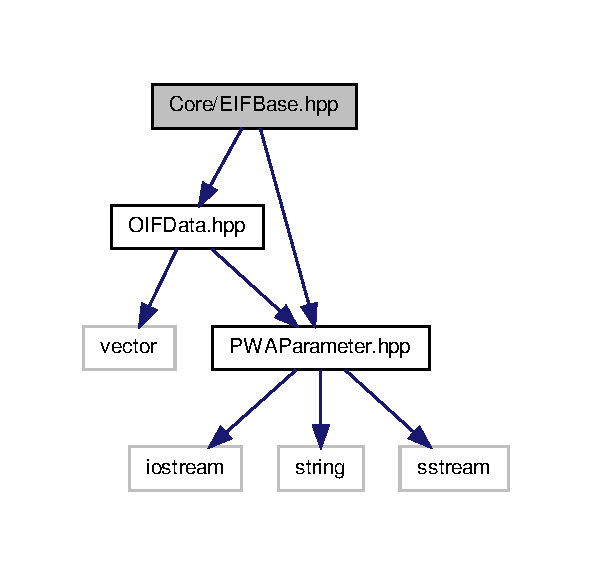
\includegraphics[width=284pt]{d5/d54/EIFBase_8hpp__incl}
\end{center}
\end{figure}
This graph shows which files directly or indirectly include this file:
\nopagebreak
\begin{figure}[H]
\begin{center}
\leavevmode
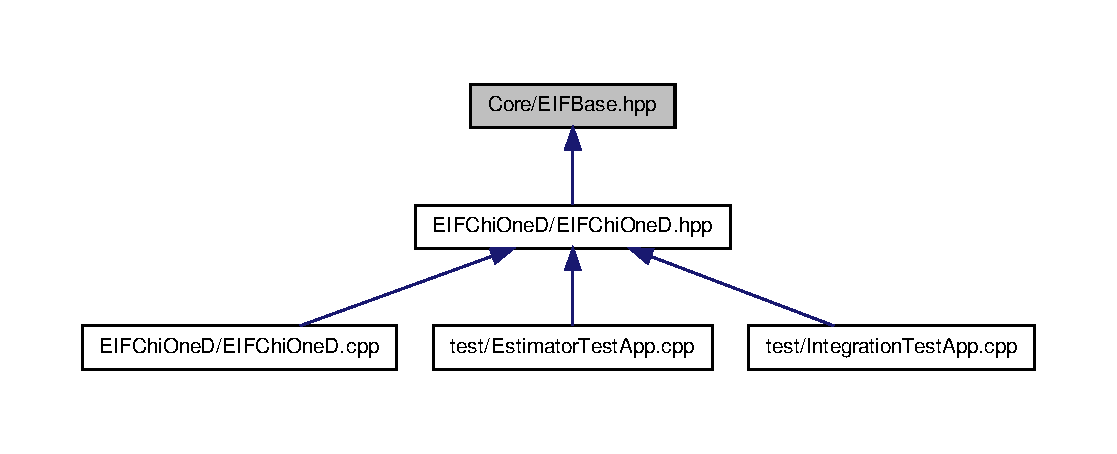
\includegraphics[width=400pt]{d7/def/EIFBase_8hpp__dep__incl}
\end{center}
\end{figure}
\subsection*{Classes}
\begin{DoxyCompactItemize}
\item 
class \hyperlink{classEIFBase}{EIFBase}
\begin{DoxyCompactList}\small\item\em Estimator Interface Base-\/Class. \end{DoxyCompactList}\end{DoxyCompactItemize}


\subsection{Detailed Description}
This class provides the interface to classes which estimate the \char`\"{}closeness\char`\"{} of the modeled intensity to the data. As it is pure virtual, one needs at least one implementation to provide an estimator for the analysis. If a new estimator is derived from and fulfills this base-\/class, no change in other modules are necessary to work with the new estimation function. As it is derived from \hyperlink{classOIFData}{OIFData}, it can be used in the optimizer modules. 
\hypertarget{OIFBase_8hpp}{
\section{Core/OIFBase.hpp File Reference}
\label{d8/dc8/OIFBase_8hpp}\index{Core/OIFBase.hpp@{Core/OIFBase.hpp}}
}


This class provides the interface to (external) optimization libraries or routines.  


\subsection*{Classes}
\begin{DoxyCompactItemize}
\item 
class \hyperlink{classOIFBase}{OIFBase}
\begin{DoxyCompactList}\small\item\em Optimizer Interface Base-\/Class. \end{DoxyCompactList}\end{DoxyCompactItemize}


\subsection{Detailed Description}
This class provides the interface to (external) optimization libraries or routines. As it is pure virtual, one needs at least one implementation to provide an optimizer for the analysis which varies free model-\/parameters. If a new optimizer is derived from and fulfills this base-\/class, no change in other modules are necessary to work with the new optimizer library or routine. 
\hypertarget{OIFData_8hpp}{
\section{Core/OIFData.hpp File Reference}
\label{db/dc2/OIFData_8hpp}\index{Core/OIFData.hpp@{Core/OIFData.hpp}}
}


This class provides the interface for the optimizer module to access the data.  


{\ttfamily \#include $<$vector$>$}\par
\subsection*{Classes}
\begin{DoxyCompactItemize}
\item 
class \hyperlink{classOIFData}{OIFData}
\begin{DoxyCompactList}\small\item\em Optimizer Data Base-\/Class. \end{DoxyCompactList}\end{DoxyCompactItemize}


\subsection{Detailed Description}
This class provides the interface for the optimizer module to access the data. If the access to the data is provided fulfilling this interface, then one can use the same data and parameter-\/set with different optimizers. 
\hypertarget{PIFBase_8hpp}{
\section{Core/PIFBase.hpp File Reference}
\label{de/dc5/PIFBase_8hpp}\index{Core/PIFBase.hpp@{Core/PIFBase.hpp}}
}


This class provides the interface to the model which tries to describe the intensity.  


{\ttfamily \#include $<$vector$>$}\par
{\ttfamily \#include \char`\"{}PWAParameter.hpp\char`\"{}}\par
Include dependency graph for PIFBase.hpp:\nopagebreak
\begin{figure}[H]
\begin{center}
\leavevmode
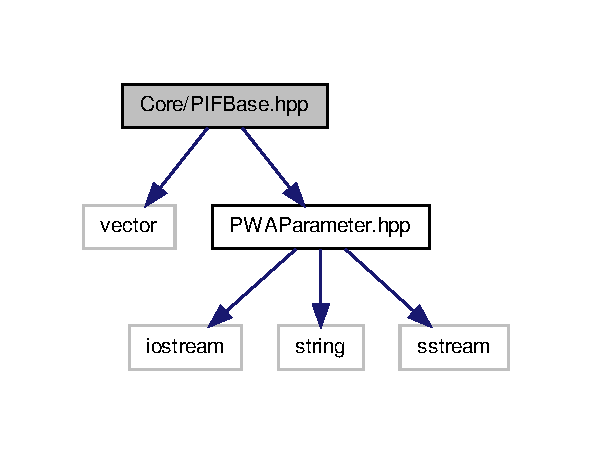
\includegraphics[width=284pt]{d9/d58/PIFBase_8hpp__incl}
\end{center}
\end{figure}
This graph shows which files directly or indirectly include this file:
\nopagebreak
\begin{figure}[H]
\begin{center}
\leavevmode
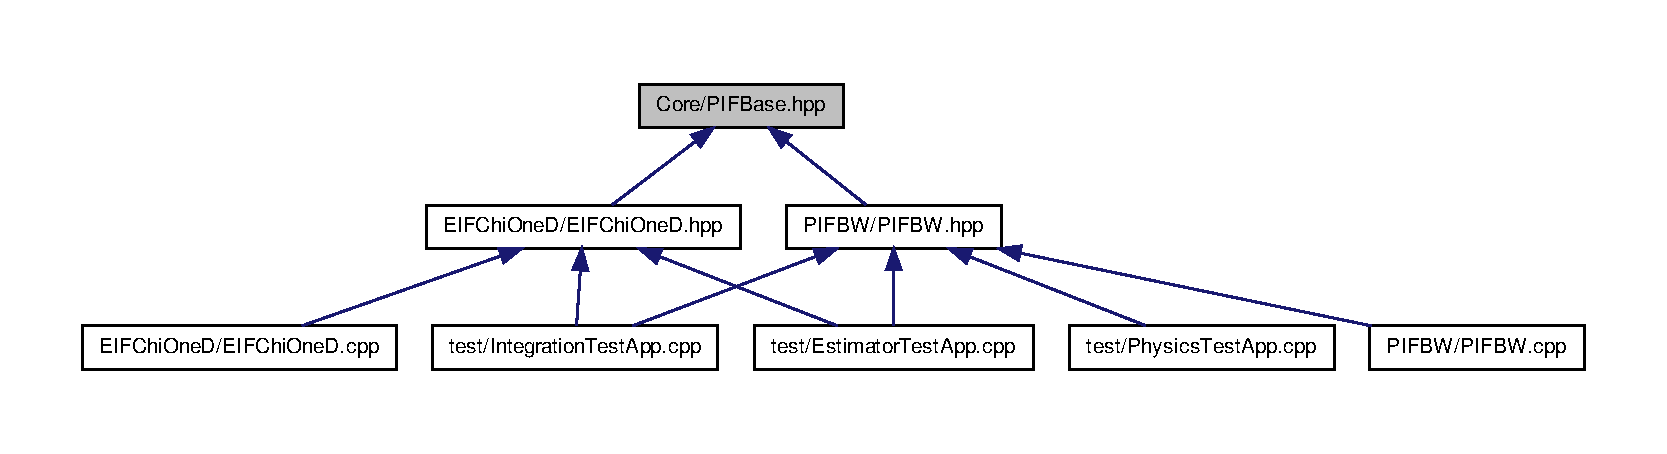
\includegraphics[width=400pt]{d1/da3/PIFBase_8hpp__dep__incl}
\end{center}
\end{figure}
\subsection*{Classes}
\begin{DoxyCompactItemize}
\item 
class \hyperlink{classPIFBase}{PIFBase}
\begin{DoxyCompactList}\small\item\em Physics Interface Base-\/Class. \end{DoxyCompactList}\end{DoxyCompactItemize}


\subsection{Detailed Description}
This class provides the interface to the model which tries to describe the intensity. As it is pure virtual, one needs at least one implementation to provide an model for the analysis which calculates intensities for an event on basis model parameters. If a new physics-\/model is derived from and fulfills this base-\/class, no change in other modules are necessary to work with the new physics module. 
\hypertarget{PWAEvent_8cpp}{
\section{Core/PWAEvent.cpp File Reference}
\label{dd/d04/PWAEvent_8cpp}\index{Core/PWAEvent.cpp@{Core/PWAEvent.cpp}}
}
{\ttfamily \#include $<$vector$>$}\par
{\ttfamily \#include \char`\"{}PWAParticle.hpp\char`\"{}}\par
{\ttfamily \#include \char`\"{}PWAEvent.hpp\char`\"{}}\par
Include dependency graph for PWAEvent.cpp:\nopagebreak
\begin{figure}[H]
\begin{center}
\leavevmode
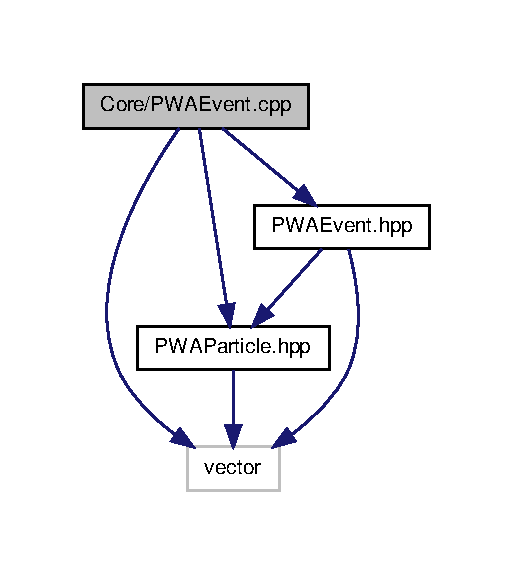
\includegraphics[width=246pt]{d2/dad/PWAEvent_8cpp__incl}
\end{center}
\end{figure}

\hypertarget{PWAEvent_8hpp}{
\section{Core/PWAEvent.hpp File Reference}
\label{d8/d14/PWAEvent_8hpp}\index{Core/PWAEvent.hpp@{Core/PWAEvent.hpp}}
}


This class provides a internal container for event-\/based information.  


{\ttfamily \#include $<$vector$>$}\par
{\ttfamily \#include \char`\"{}PWAParticle.hpp\char`\"{}}\par
Include dependency graph for PWAEvent.hpp:\nopagebreak
\begin{figure}[H]
\begin{center}
\leavevmode
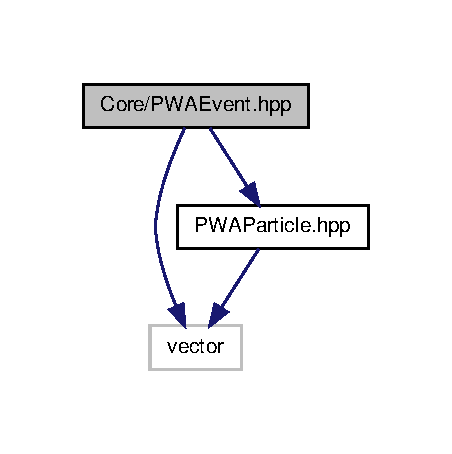
\includegraphics[width=217pt]{d1/dfe/PWAEvent_8hpp__incl}
\end{center}
\end{figure}
This graph shows which files directly or indirectly include this file:
\nopagebreak
\begin{figure}[H]
\begin{center}
\leavevmode
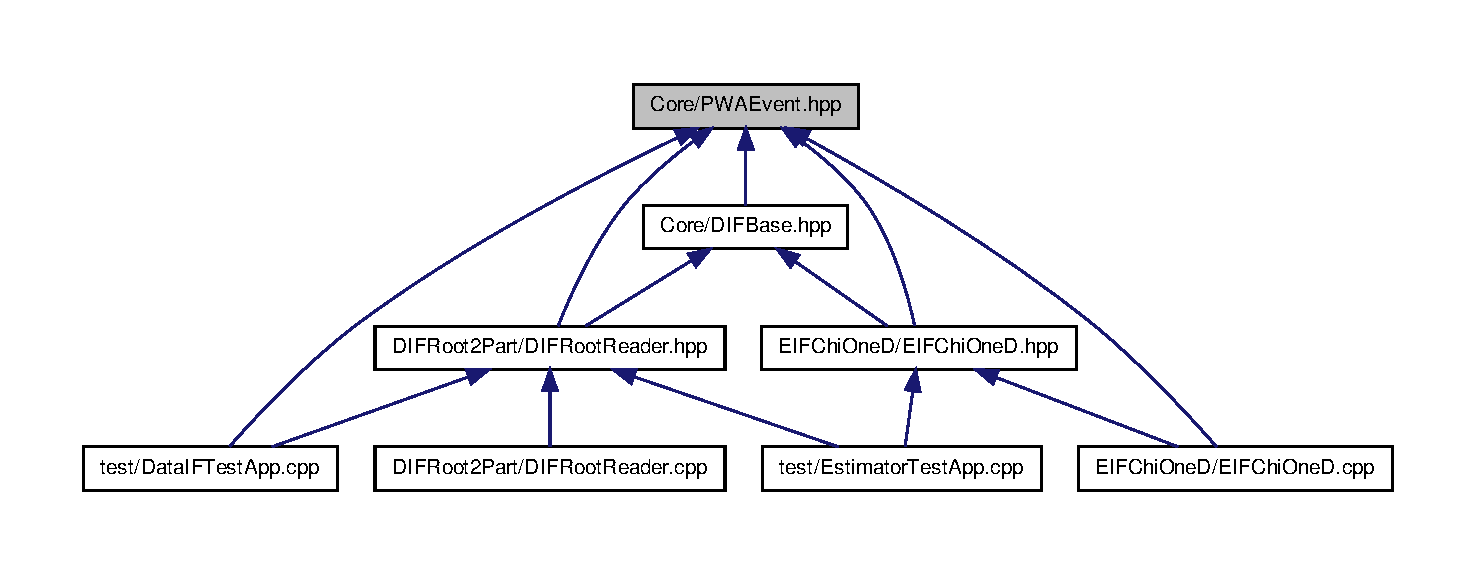
\includegraphics[width=400pt]{d4/dc4/PWAEvent_8hpp__dep__incl}
\end{center}
\end{figure}
\subsection*{Classes}
\begin{DoxyCompactItemize}
\item 
class \hyperlink{classPWAEvent}{PWAEvent}
\begin{DoxyCompactList}\small\item\em Internal container for event information. \end{DoxyCompactList}\end{DoxyCompactItemize}


\subsection{Detailed Description}
This class provides a internal container for event-\/based information. The class provides a list of particles of the event. 
\hypertarget{PWAParameter_8hpp}{
\section{Core/PWAParameter.hpp File Reference}
\label{d1/d85/PWAParameter_8hpp}\index{Core/PWAParameter.hpp@{Core/PWAParameter.hpp}}
}


This class provides a internal container for information of a fit parameter.  


{\ttfamily \#include $<$iostream$>$}\par
{\ttfamily \#include $<$string$>$}\par
{\ttfamily \#include $<$sstream$>$}\par
Include dependency graph for PWAParameter.hpp:\nopagebreak
\begin{figure}[H]
\begin{center}
\leavevmode
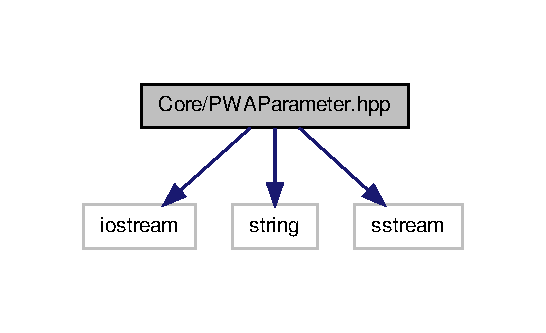
\includegraphics[width=262pt]{d9/d99/PWAParameter_8hpp__incl}
\end{center}
\end{figure}
This graph shows which files directly or indirectly include this file:
\nopagebreak
\begin{figure}[H]
\begin{center}
\leavevmode
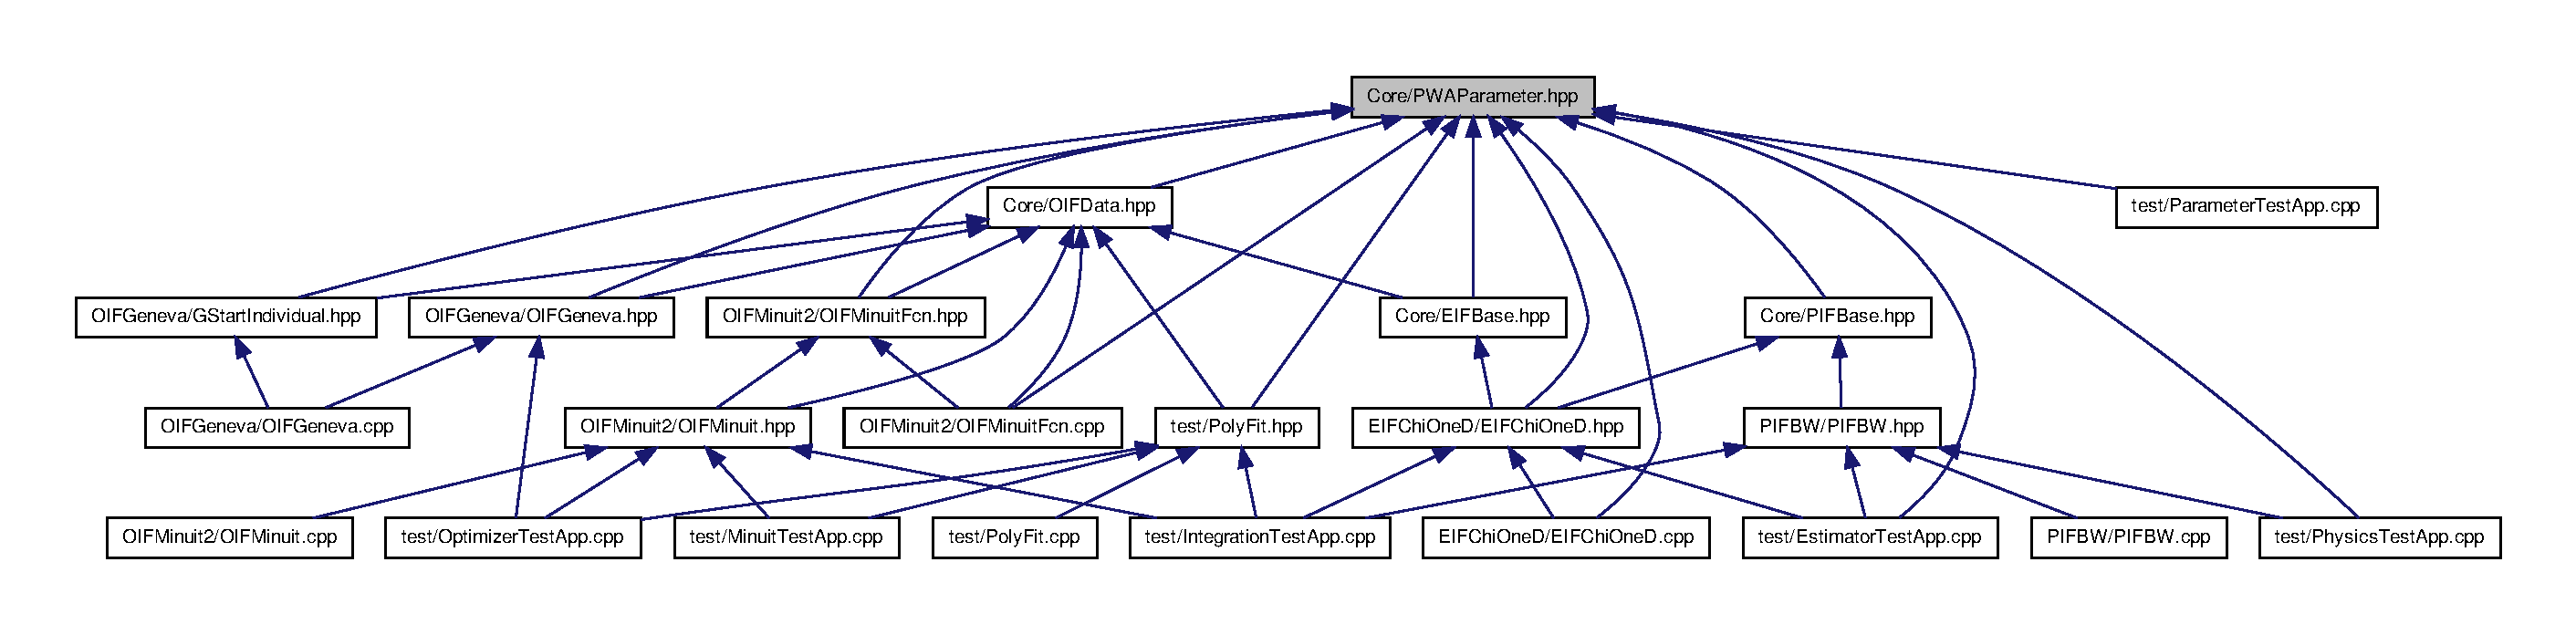
\includegraphics[width=400pt]{d2/da8/PWAParameter_8hpp__dep__incl}
\end{center}
\end{figure}
\subsection*{Classes}
\begin{DoxyCompactItemize}
\item 
class \hyperlink{classPWAParameter}{PWAParameter$<$ T $>$}
\begin{DoxyCompactList}\small\item\em Internal container representing a parameter. \end{DoxyCompactList}\end{DoxyCompactItemize}
\subsection*{Functions}
\begin{DoxyCompactItemize}
\item 
{\footnotesize template$<$class U $>$ }\\std::ostream \& \hyperlink{PWAParameter_8hpp_a22f81859f3803c4acbd53ccf03d50780}{operator$<$$<$} (std::ostream \&os, const \hyperlink{classPWAParameter}{PWAParameter}$<$ U $>$ \&p)
\end{DoxyCompactItemize}


\subsection{Detailed Description}
This class provides a internal container for information of a fit parameter. The class provides the value, bounds and error of a parameter. 

\subsection{Function Documentation}
\hypertarget{PWAParameter_8hpp_a22f81859f3803c4acbd53ccf03d50780}{
\index{PWAParameter.hpp@{PWAParameter.hpp}!operator$<$$<$@{operator$<$$<$}}
\index{operator$<$$<$@{operator$<$$<$}!PWAParameter.hpp@{PWAParameter.hpp}}
\subsubsection[{operator$<$$<$}]{\setlength{\rightskip}{0pt plus 5cm}template$<$class U $>$ std::ostream\& operator$<$$<$ (
\begin{DoxyParamCaption}
\item[{std::ostream \&}]{os, }
\item[{const {\bf PWAParameter}$<$ U $>$ \&}]{p}
\end{DoxyParamCaption}
)}}
\label{d1/d85/PWAParameter_8hpp_a22f81859f3803c4acbd53ccf03d50780}

\hypertarget{PWAParticle_8hpp}{
\section{Core/PWAParticle.hpp File Reference}
\label{d3/ded/PWAParticle_8hpp}\index{Core/PWAParticle.hpp@{Core/PWAParticle.hpp}}
}


This class provides a internal container for information of a particle.  


{\ttfamily \#include $<$vector$>$}\par
Include dependency graph for PWAParticle.hpp:
\nopagebreak
\begin{figure}[H]
\begin{center}
\leavevmode
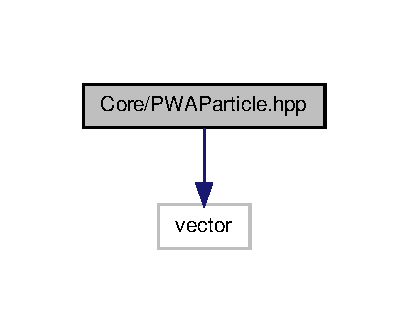
\includegraphics[width=196pt]{d1/d3d/PWAParticle_8hpp__incl}
\end{center}
\end{figure}
This graph shows which files directly or indirectly include this file:
\nopagebreak
\begin{figure}[H]
\begin{center}
\leavevmode
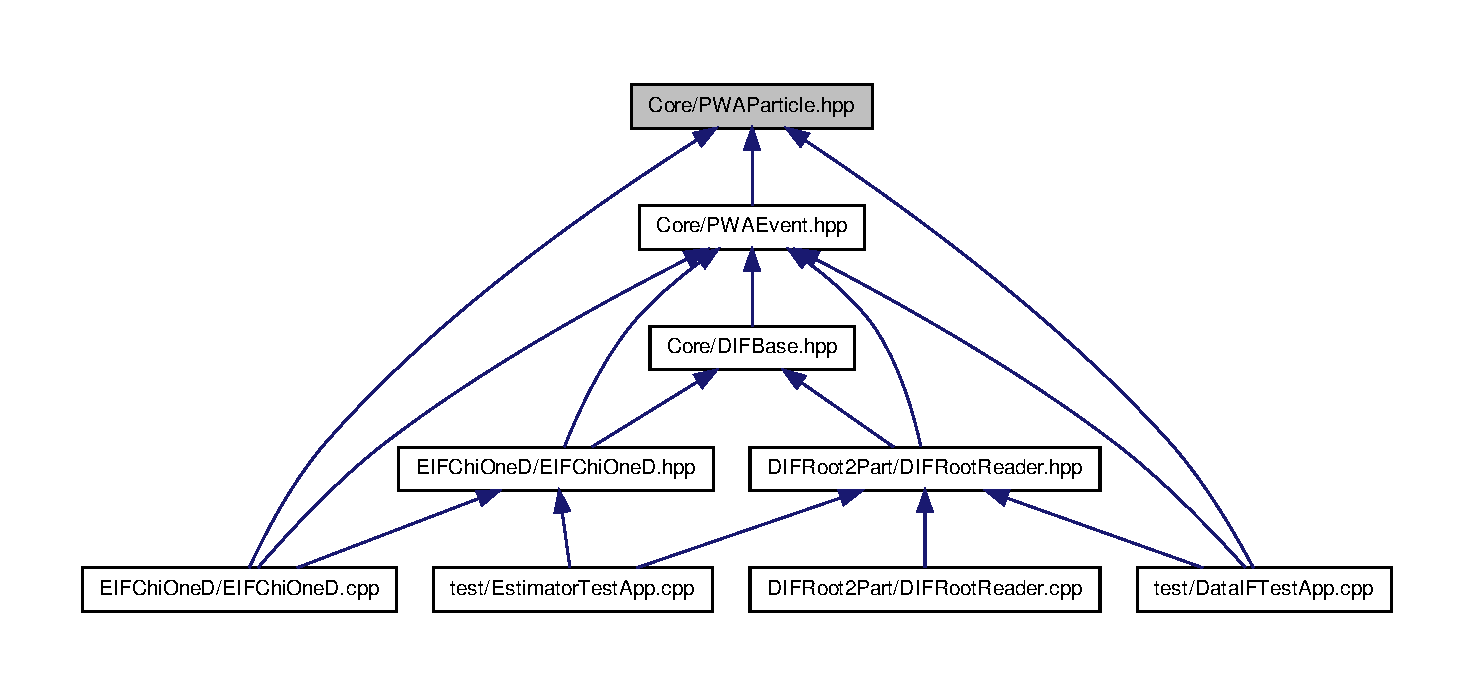
\includegraphics[width=400pt]{d1/d53/PWAParticle_8hpp__dep__incl}
\end{center}
\end{figure}
\subsection*{Classes}
\begin{DoxyCompactItemize}
\item 
class \hyperlink{classPWAParticle}{PWAParticle}
\begin{DoxyCompactList}\small\item\em Internal container representing a particle. \end{DoxyCompactList}\end{DoxyCompactItemize}


\subsection{Detailed Description}
This class provides a internal container for information of a particle. The class provides the momentum 4-\/vector and pid of the particle. 
\hypertarget{DIFRootReader_8cpp}{
\section{DIFRoot2Part/DIFRootReader.cpp File Reference}
\label{dd/de5/DIFRootReader_8cpp}\index{DIFRoot2Part/DIFRootReader.cpp@{DIFRoot2Part/DIFRootReader.cpp}}
}
{\ttfamily \#include $<$sstream$>$}\par
{\ttfamily \#include $<$iostream$>$}\par
{\ttfamily \#include $<$memory$>$}\par
{\ttfamily \#include $<$vector$>$}\par
{\ttfamily \#include \char`\"{}DIFRootReader.hpp\char`\"{}}\par
{\ttfamily \#include \char`\"{}TParticle.h\char`\"{}}\par

\hypertarget{DIFRootReader_8hpp}{
\section{DIFRoot2Part/DIFRootReader.hpp File Reference}
\label{db/d3e/DIFRootReader_8hpp}\index{DIFRoot2Part/DIFRootReader.hpp@{DIFRoot2Part/DIFRootReader.hpp}}
}


This class reads event-\/based data from root-\/files.  


{\ttfamily \#include $<$vector$>$}\par
{\ttfamily \#include $<$memory$>$}\par
{\ttfamily \#include $<$string$>$}\par
{\ttfamily \#include \char`\"{}DIFBase.hpp\char`\"{}}\par
{\ttfamily \#include \char`\"{}PWAEvent.hpp\char`\"{}}\par
{\ttfamily \#include \char`\"{}TMath.h\char`\"{}}\par
{\ttfamily \#include \char`\"{}TLorentzVector.h\char`\"{}}\par
{\ttfamily \#include \char`\"{}TParticle.h\char`\"{}}\par
{\ttfamily \#include \char`\"{}TROOT.h\char`\"{}}\par
{\ttfamily \#include \char`\"{}TFile.h\char`\"{}}\par
{\ttfamily \#include \char`\"{}TClonesArray.h\char`\"{}}\par
{\ttfamily \#include \char`\"{}TTree.h\char`\"{}}\par
{\ttfamily \#include \char`\"{}TRandom3.h\char`\"{}}\par
Include dependency graph for DIFRootReader.hpp:
\nopagebreak
\begin{figure}[H]
\begin{center}
\leavevmode
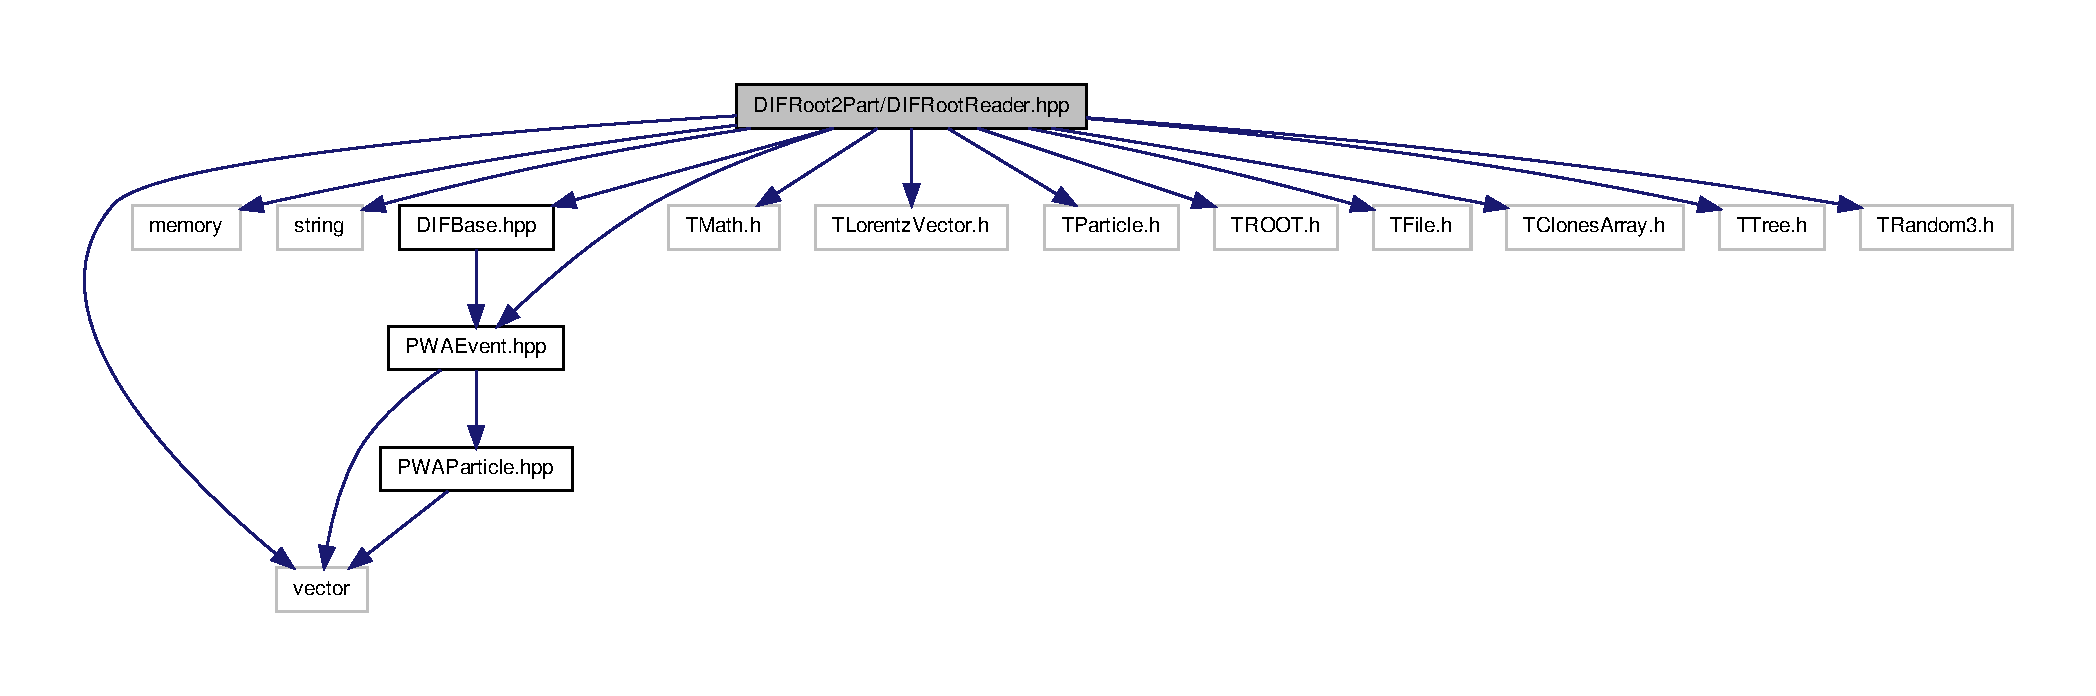
\includegraphics[width=400pt]{d8/d40/DIFRootReader_8hpp__incl}
\end{center}
\end{figure}
This graph shows which files directly or indirectly include this file:
\nopagebreak
\begin{figure}[H]
\begin{center}
\leavevmode
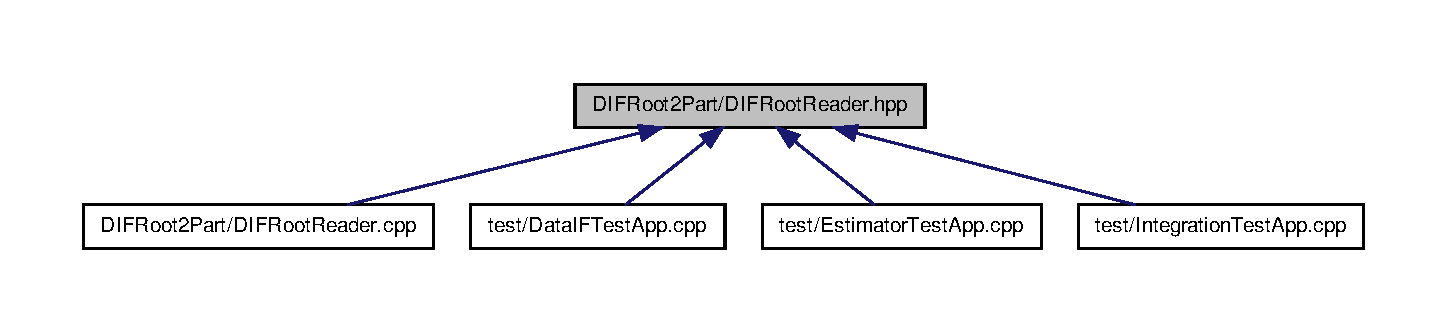
\includegraphics[width=400pt]{da/d34/DIFRootReader_8hpp__dep__incl}
\end{center}
\end{figure}
\subsection*{Classes}
\begin{DoxyCompactItemize}
\item 
class \hyperlink{classDIFRootReader}{DIFRootReader}
\begin{DoxyCompactList}\small\item\em Reader for data in Root-\/files. \end{DoxyCompactList}\end{DoxyCompactItemize}


\subsection{Detailed Description}
This class reads event-\/based data from root-\/files. It implements the interface of \hyperlink{DIFBase_8hpp}{DIFBase.hpp}. 
\hypertarget{EIFChiOneD_8cpp}{
\section{EIFChiOneD/EIFChiOneD.cpp File Reference}
\label{d8/d80/EIFChiOneD_8cpp}\index{EIFChiOneD/EIFChiOneD.cpp@{EIFChiOneD/EIFChiOneD.cpp}}
}
{\ttfamily \#include $<$sstream$>$}\par
{\ttfamily \#include $<$iostream$>$}\par
{\ttfamily \#include $<$memory$>$}\par
{\ttfamily \#include $<$vector$>$}\par
{\ttfamily \#include $<$cmath$>$}\par
{\ttfamily \#include \char`\"{}EIFChiOneD.hpp\char`\"{}}\par
{\ttfamily \#include \char`\"{}PWAEvent.hpp\char`\"{}}\par
{\ttfamily \#include \char`\"{}PWAParticle.hpp\char`\"{}}\par
{\ttfamily \#include \char`\"{}PWAParameter.hpp\char`\"{}}\par
Include dependency graph for EIFChiOneD.cpp:\nopagebreak
\begin{figure}[H]
\begin{center}
\leavevmode
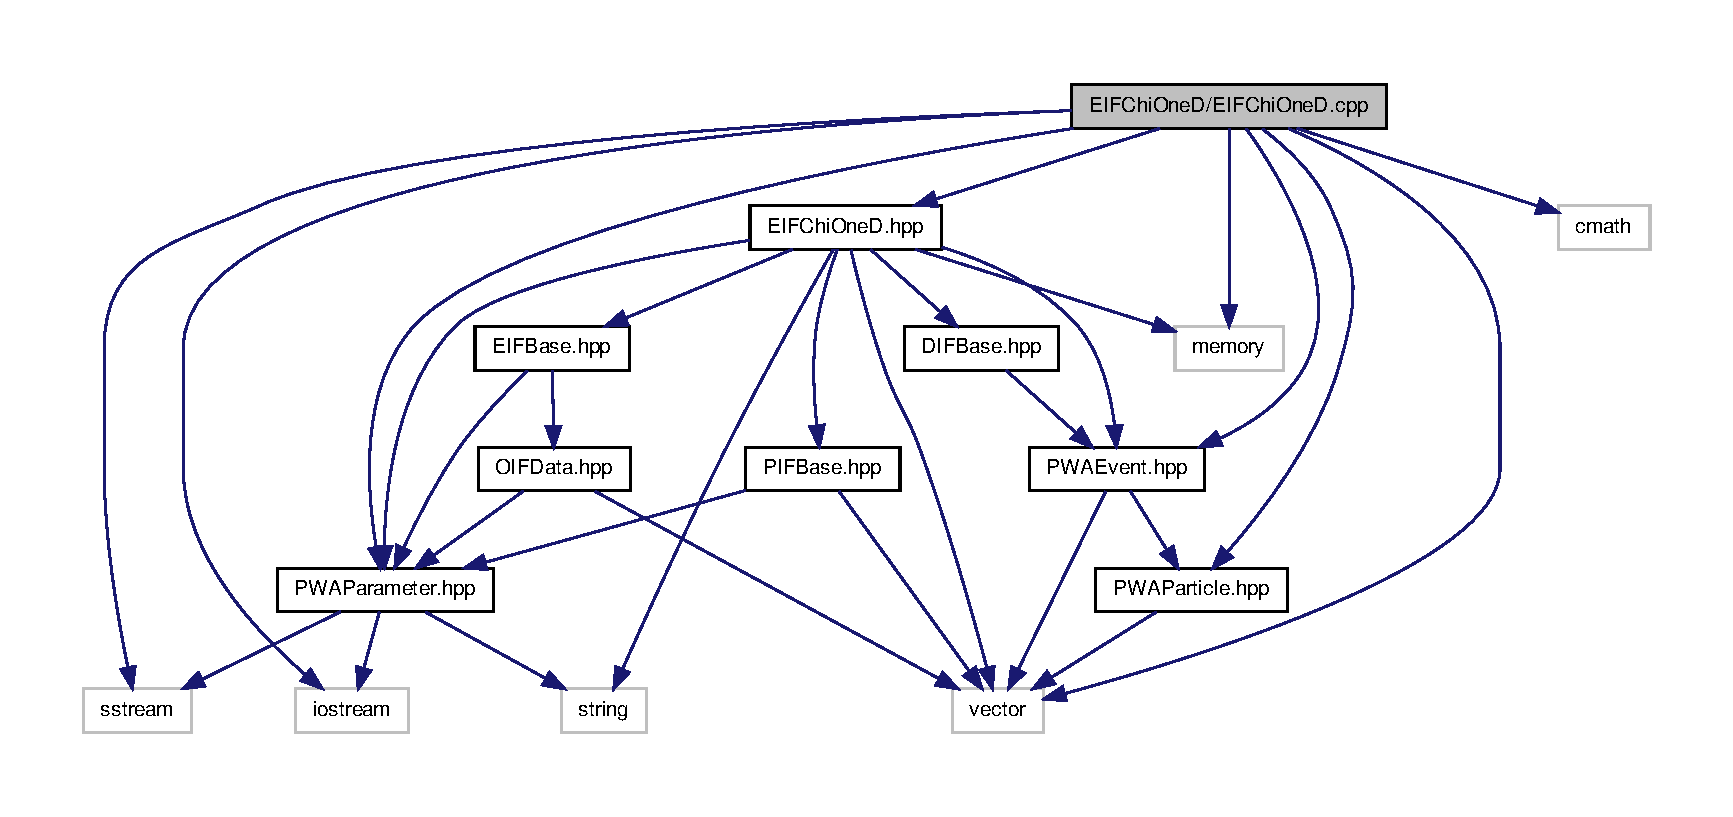
\includegraphics[width=400pt]{dc/d0c/EIFChiOneD_8cpp__incl}
\end{center}
\end{figure}

\hypertarget{EIFChiOneD_8hpp}{
\section{EIFChiOneD/EIFChiOneD.hpp File Reference}
\label{d3/d5d/EIFChiOneD_8hpp}\index{EIFChiOneD/EIFChiOneD.hpp@{EIFChiOneD/EIFChiOneD.hpp}}
}


This class calculates a simple $\chi^{2}$ of a intensity and a dataset.  


{\ttfamily \#include $<$vector$>$}\par
{\ttfamily \#include $<$memory$>$}\par
{\ttfamily \#include $<$string$>$}\par
{\ttfamily \#include \char`\"{}EIFBase.hpp\char`\"{}}\par
{\ttfamily \#include \char`\"{}PIFBase.hpp\char`\"{}}\par
{\ttfamily \#include \char`\"{}DIFBase.hpp\char`\"{}}\par
{\ttfamily \#include \char`\"{}PWAEvent.hpp\char`\"{}}\par
{\ttfamily \#include \char`\"{}PWAParameter.hpp\char`\"{}}\par
Include dependency graph for EIFChiOneD.hpp:\nopagebreak
\begin{figure}[H]
\begin{center}
\leavevmode
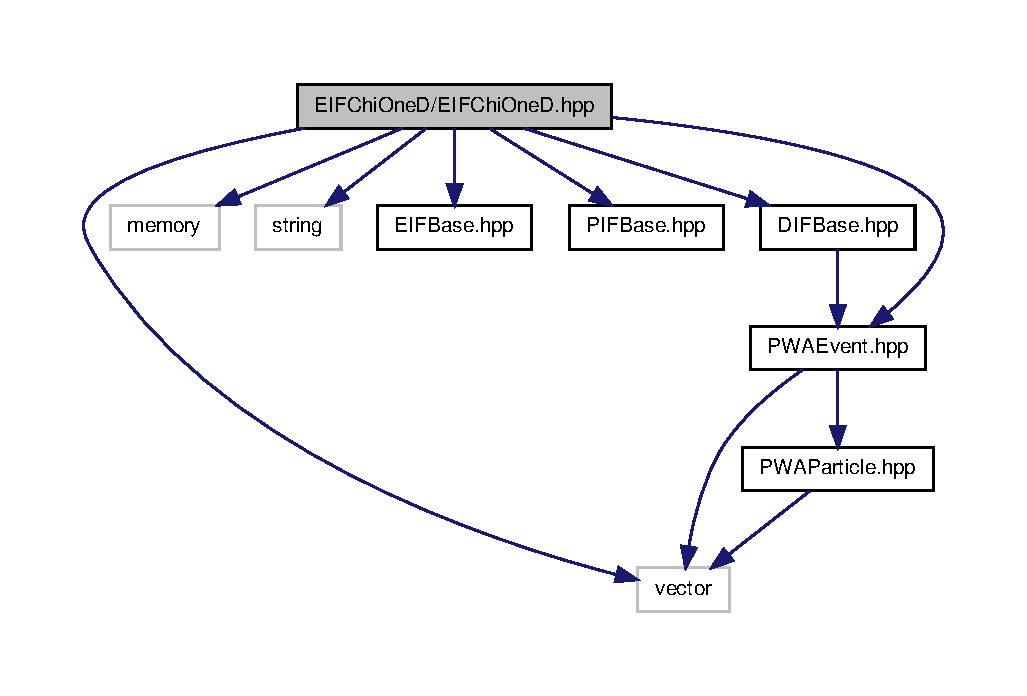
\includegraphics[width=400pt]{d9/d3e/EIFChiOneD_8hpp__incl}
\end{center}
\end{figure}
This graph shows which files directly or indirectly include this file:
\nopagebreak
\begin{figure}[H]
\begin{center}
\leavevmode
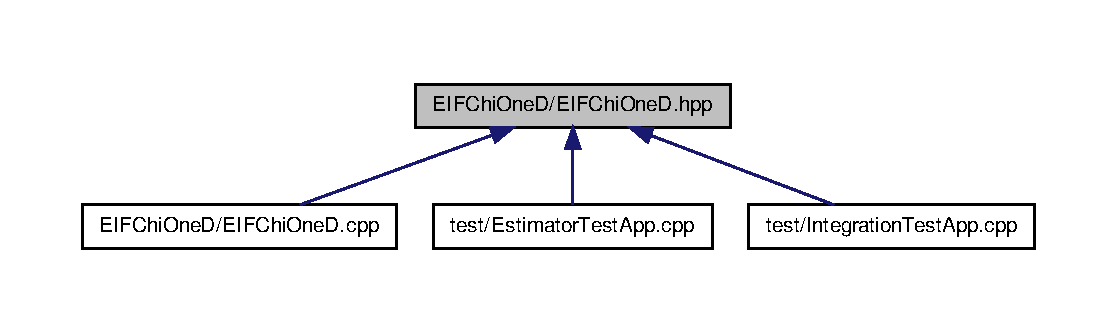
\includegraphics[width=400pt]{d0/dd8/EIFChiOneD_8hpp__dep__incl}
\end{center}
\end{figure}
\subsection*{Classes}
\begin{DoxyCompactItemize}
\item 
class \hyperlink{classEIFChiOneD}{EIFChiOneD}
\begin{DoxyCompactList}\small\item\em Simple $\chi^{2}$-\/Estimator. \end{DoxyCompactList}\end{DoxyCompactItemize}


\subsection{Detailed Description}
This class calculates a simple $\chi^{2}$ of a intensity and a dataset. Data and Model are provided in the constructor using the \hyperlink{classPIFBase}{PIFBase} and \hyperlink{classDIFBase}{DIFBase} interfaces. The class itself fulfills the \hyperlink{classEIFBase}{EIFBase} interface. 
\hypertarget{GArgumentParser_8cpp}{
\section{OIFGeneva/GArgumentParser.cpp File Reference}
\label{d5/d42/GArgumentParser_8cpp}\index{OIFGeneva/GArgumentParser.cpp@{OIFGeneva/GArgumentParser.cpp}}
}
{\ttfamily \#include \char`\"{}GArgumentParser.hpp\char`\"{}}\par
Include dependency graph for GArgumentParser.cpp:\nopagebreak
\begin{figure}[H]
\begin{center}
\leavevmode
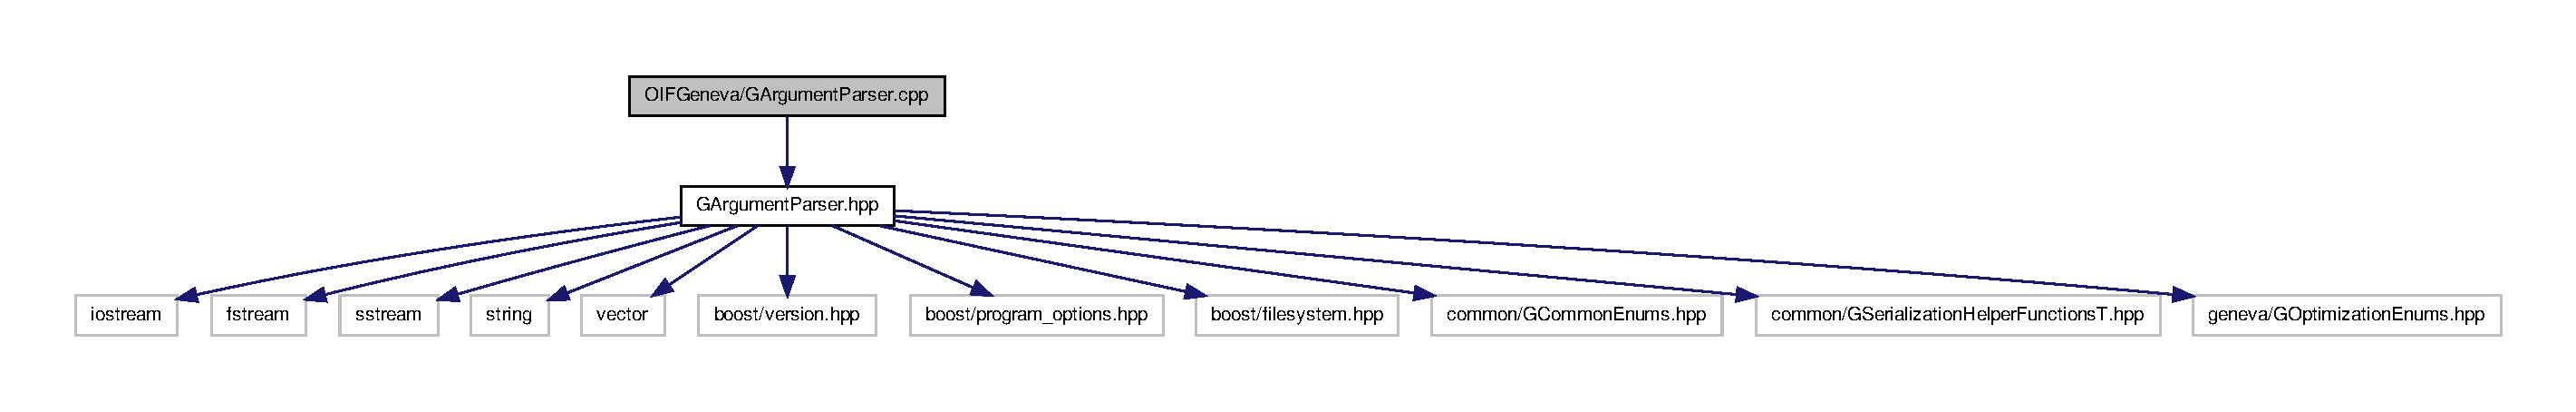
\includegraphics[width=400pt]{d7/dfb/GArgumentParser_8cpp__incl}
\end{center}
\end{figure}
\subsection*{Namespaces}
\begin{DoxyCompactItemize}
\item 
namespace \hyperlink{namespaceGem}{Gem}
\item 
namespace \hyperlink{namespaceGem_1_1Geneva}{Gem::Geneva}
\end{DoxyCompactItemize}
\subsection*{Functions}
\begin{DoxyCompactItemize}
\item 
bool \hyperlink{namespaceGem_1_1Geneva_a32eaed60d47903f4584394f0ceb6567c}{Gem::Geneva::parseCommandLine} (int argc, char $\ast$$\ast$argv, std::string \&configFile, boost::uint16\_\-t \&parallelizationMode, bool \&serverMode, std::string \&ip, unsigned short \&port, Gem::Common::serializationMode \&serMode)
\item 
bool \hyperlink{namespaceGem_1_1Geneva_a72bec142348625258508d6cb05700395}{Gem::Geneva::parseConfigFile} (const std::string \&configFile, boost::uint16\_\-t \&nProducerThreads, boost::uint16\_\-t \&nEvaluationThreads, std::size\_\-t \&populationSize, std::size\_\-t \&nParents, boost::uint32\_\-t \&maxIterations, long \&maxMinutes, boost::uint32\_\-t \&reportIteration, recoScheme \&rScheme, sortingMode \&smode, std::size\_\-t \&arraySize, boost::uint32\_\-t \&processingCycles, bool \&returnRegardless, boost::uint32\_\-t \&waitFactor)
\end{DoxyCompactItemize}


\subsection{Detailed Description}

\hypertarget{GArgumentParser_8hpp}{
\section{OIFGeneva/GArgumentParser.hpp File Reference}
\label{d4/d3c/GArgumentParser_8hpp}\index{OIFGeneva/GArgumentParser.hpp@{OIFGeneva/GArgumentParser.hpp}}
}


Geneva argument parser to interpret command line arguments and config files.  


{\ttfamily \#include $<$iostream$>$}\par
{\ttfamily \#include $<$fstream$>$}\par
{\ttfamily \#include $<$sstream$>$}\par
{\ttfamily \#include $<$string$>$}\par
{\ttfamily \#include $<$vector$>$}\par
{\ttfamily \#include $<$boost/version.hpp$>$}\par
{\ttfamily \#include $<$boost/program\_\-options.hpp$>$}\par
{\ttfamily \#include $<$boost/filesystem.hpp$>$}\par
{\ttfamily \#include $<$common/GCommonEnums.hpp$>$}\par
{\ttfamily \#include $<$common/GSerializationHelperFunctionsT.hpp$>$}\par
{\ttfamily \#include $<$geneva/GOptimizationEnums.hpp$>$}\par
\subsection*{Namespaces}
\begin{DoxyCompactItemize}
\item 
namespace \hyperlink{namespaceGem}{Gem}
\item 
namespace \hyperlink{namespaceGem_1_1Geneva}{Gem::Geneva}
\end{DoxyCompactItemize}
\subsection*{Functions}
\begin{DoxyCompactItemize}
\item 
bool \hyperlink{namespaceGem_1_1Geneva_a32eaed60d47903f4584394f0ceb6567c}{Gem::Geneva::parseCommandLine} (int argc, char $\ast$$\ast$argv, std::string \&configFile, boost::uint16\_\-t \&parallelizationMode, bool \&serverMode, std::string \&ip, unsigned short \&port, Gem::Common::serializationMode \&serMode)
\item 
bool \hyperlink{namespaceGem_1_1Geneva_a72bec142348625258508d6cb05700395}{Gem::Geneva::parseConfigFile} (const std::string \&configFile, boost::uint16\_\-t \&nProducerThreads, boost::uint16\_\-t \&nEvaluationThreads, std::size\_\-t \&populationSize, std::size\_\-t \&nParents, boost::uint32\_\-t \&maxIterations, long \&maxMinutes, boost::uint32\_\-t \&reportIteration, recoScheme \&rScheme, sortingMode \&smode, std::size\_\-t \&arraySize, boost::uint32\_\-t \&processingCycles, bool \&returnRegardless, boost::uint32\_\-t \&waitFactor)
\end{DoxyCompactItemize}
\subsection*{Variables}
\begin{DoxyCompactItemize}
\item 
const boost::uint16\_\-t \hyperlink{namespaceGem_1_1Geneva_a505a99cdd13909343ea78ab3bdf56474}{Gem::Geneva::DEFAULTNPRODUCERTHREADS} = 10
\item 
const boost::uint16\_\-t \hyperlink{namespaceGem_1_1Geneva_a86f3fe2eb8311d0a9b5c18a32c8ee4f1}{Gem::Geneva::DEFAULTNEVALUATIONTHREADS} = 4
\item 
const std::size\_\-t \hyperlink{namespaceGem_1_1Geneva_a09727ec1a0c3212b45a43896ba422151}{Gem::Geneva::DEFAULTPOPULATIONSIZE} = 100
\item 
const std::size\_\-t \hyperlink{namespaceGem_1_1Geneva_a7ba466fb273415c31b26532094f2dd51}{Gem::Geneva::DEFAULTNPARENTS} = 5
\item 
const boost::uint32\_\-t \hyperlink{namespaceGem_1_1Geneva_a71dd5f6f26fa4f040b16cc729074f219}{Gem::Geneva::DEFAULTMAXITERATIONS} = 2000
\item 
const long \hyperlink{namespaceGem_1_1Geneva_a84c4227f18d85106f2377e8f5cbddf4d}{Gem::Geneva::DEFAULTMAXMINUTES} = 10
\item 
const boost::uint32\_\-t \hyperlink{namespaceGem_1_1Geneva_a2b3f870846aa6ccf4502b14e837707d4}{Gem::Geneva::DEFAULTREPORTITERATION} = 1
\item 
const recoScheme \hyperlink{namespaceGem_1_1Geneva_abf07d2c9bf8cc79475a14f410e435cd0}{Gem::Geneva::DEFAULTRSCHEME} = VALUERECOMBINE
\item 
const bool \hyperlink{namespaceGem_1_1Geneva_acfa46336c5707f08a2ef1e87fde2ba4d}{Gem::Geneva::DEFAULTVERBOSE} = true
\item 
const bool \hyperlink{namespaceGem_1_1Geneva_a0d079f912cda83149347effa10cc7039}{Gem::Geneva::DEFAULTPARALLELIZATIONMODE} = 1
\item 
const std::size\_\-t \hyperlink{namespaceGem_1_1Geneva_ad46712aab7136ab7e747ea8860ab46ff}{Gem::Geneva::DEFAULTARRAYSIZE} = 1000
\item 
const bool \hyperlink{namespaceGem_1_1Geneva_ae70305897c4fb0100476012f61c32ae9}{Gem::Geneva::DEFAULTPRODUCTIONPLACE} = true
\item 
const bool \hyperlink{namespaceGem_1_1Geneva_ae66444afbff6f0454a6f7087d0b9ee0a}{Gem::Geneva::DEFAULTUSECOMMONADAPTOR} = false
\item 
const unsigned short \hyperlink{namespaceGem_1_1Geneva_ab35a5c233444f13095b80a36270de007}{Gem::Geneva::DEFAULTPORT} = 10000
\item 
const std::string \hyperlink{namespaceGem_1_1Geneva_a06037b35202b3efd9e20000d566bd790}{Gem::Geneva::DEFAULTIP} = \char`\"{}localhost\char`\"{}
\item 
const std::string \hyperlink{namespaceGem_1_1Geneva_aaba4e2cd93c01787464ebd89699a0259}{Gem::Geneva::DEFAULTCONFIGFILE} = \char`\"{}./GStartProject.cfg\char`\"{}
\item 
const sortingMode \hyperlink{namespaceGem_1_1Geneva_ae75bab36ebf398bfef62bc0432280980}{Gem::Geneva::DEFAULTSORTINGSCHEME} = MUPLUSNU
\item 
const boost::uint32\_\-t \hyperlink{namespaceGem_1_1Geneva_a1295783da2a3d26bd95ee66a2b1e0e28}{Gem::Geneva::DEFAULTSTARTITERATION} = 0
\item 
const boost::uint32\_\-t \hyperlink{namespaceGem_1_1Geneva_a6c15979db3e3fb1efa968e5444296b01}{Gem::Geneva::DEFAULTPROCESSINGCYCLES} = 1
\item 
const bool \hyperlink{namespaceGem_1_1Geneva_aa28d6ada86d874ce11bde88b5569a34d}{Gem::Geneva::DEFAULTRETURNREGARDLESS} = true
\item 
const std::size\_\-t \hyperlink{namespaceGem_1_1Geneva_ac381bed98f84863017b49a4c155199fe}{Gem::Geneva::DEFAULTNBTCONSUMERTHREADS} = 2
\item 
const boost::uint32\_\-t \hyperlink{namespaceGem_1_1Geneva_a1a77f7000b4cb6095f973fc2d0571ff9}{Gem::Geneva::DEFAULTGBTCWAITFACTOR} = 5
\item 
const Gem::Common::serializationMode \hyperlink{namespaceGem_1_1Geneva_abffd76330c5d5bbb1808dd71a3241944}{Gem::Geneva::DEFAULTSERMODE} = Gem::Common::SERIALIZATIONMODE\_\-TEXT
\end{DoxyCompactItemize}


\subsection{Detailed Description}
Geneva argument parser to interpret command line arguments and config files. Adapted for the use in ComPWA. Original Copyright see below:

Copyright (C) Gemfony scientific UG (haftungsbeschraenkt) and Karlsruhe Institute of Technology (University of the State of Baden-\/Wuerttemberg and National Laboratory of the Helmholtz Association).

See the AUTHORS file in the top-\/level directory for a list of authors.

Contact: contact \mbox{[}at\mbox{]} gemfony (dot) com

This file is part of the Geneva library collection

Geneva is free software: you can redistribute it and/or modify it under the terms of version 3 of the GNU Affero General Public License as published by the Free Software Foundation.

Geneva is distributed in the hope that it will be useful, but WITHOUT ANY WARRANTY; without even the implied warranty of MERCHANTABILITY or FITNESS FOR A PARTICULAR PURPOSE. See the GNU Affero General Public License for more details.

You should have received a copy of the GNU Affero General Public License along with the Geneva library. If not, see $<$\href{http://www.gnu.org/licenses/}{\tt http://www.gnu.org/licenses/}$>$.

For further information on Gemfony scientific and Geneva, visit \href{http://www.gemfony.com}{\tt http://www.gemfony.com} . 
\hypertarget{GStartIndividual_8hpp}{
\section{OIFGeneva/GStartIndividual.hpp File Reference}
\label{df/dfa/GStartIndividual_8hpp}\index{OIFGeneva/GStartIndividual.hpp@{OIFGeneva/GStartIndividual.hpp}}
}


Geneva individual extended to the use in ComPWA, using \hyperlink{classOIFData}{OIFData} to access the data.  


{\ttfamily \#include $<$iostream$>$}\par
{\ttfamily \#include $<$cmath$>$}\par
{\ttfamily \#include $<$cstdlib$>$}\par
{\ttfamily \#include $<$sstream$>$}\par
{\ttfamily \#include $<$vector$>$}\par
{\ttfamily \#include $<$list$>$}\par
{\ttfamily \#include $<$algorithm$>$}\par
{\ttfamily \#include $<$utility$>$}\par
{\ttfamily \#include $<$common/GGlobalDefines.hpp$>$}\par
{\ttfamily \#include $<$boost/shared\_\-ptr.hpp$>$}\par
{\ttfamily \#include $<$boost/bind.hpp$>$}\par
{\ttfamily \#include $<$boost/filesystem/operations.hpp$>$}\par
{\ttfamily \#include $<$boost/algorithm/string/trim.hpp$>$}\par
{\ttfamily \#include $<$boost/cast.hpp$>$}\par
{\ttfamily \#include $<$hap/GRandomT.hpp$>$}\par
{\ttfamily \#include $<$common/GCommonEnums.hpp$>$}\par
{\ttfamily \#include $<$common/GExceptions.hpp$>$}\par
{\ttfamily \#include $<$geneva/GConstrainedDoubleObject.hpp$>$}\par
{\ttfamily \#include $<$geneva/GConstrainedDoubleObjectCollection.hpp$>$}\par
{\ttfamily \#include $<$geneva/GDoubleGaussAdaptor.hpp$>$}\par
{\ttfamily \#include $<$geneva/GObjectExpectationChecksT.hpp$>$}\par
{\ttfamily \#include $<$geneva/GParameterObjectCollection.hpp$>$}\par
{\ttfamily \#include $<$geneva/GParameterSet.hpp$>$}\par
{\ttfamily \#include \char`\"{}OIFData.hpp\char`\"{}}\par
{\ttfamily \#include $<$boost/serialization/export.hpp$>$}\par
\subsection*{Classes}
\begin{DoxyCompactItemize}
\item 
class \hyperlink{classGem_1_1Geneva_1_1GStartIndividual}{Gem::Geneva::GStartIndividual}
\end{DoxyCompactItemize}
\subsection*{Namespaces}
\begin{DoxyCompactItemize}
\item 
namespace \hyperlink{namespaceGem}{Gem}
\item 
namespace \hyperlink{namespaceGem_1_1Geneva}{Gem::Geneva}
\end{DoxyCompactItemize}
\subsection*{Defines}
\begin{DoxyCompactItemize}
\item 
\#define \hyperlink{GStartIndividual_8hpp_a1e7025267d70bf9660d690ec7c7fc33f}{GSTARTINDIVIDUAL\_\-HPP\_\-}
\end{DoxyCompactItemize}


\subsection{Detailed Description}
Geneva individual extended to the use in ComPWA, using \hyperlink{classOIFData}{OIFData} to access the data. Original Copyright see below:

Copyright (C) Gemfony scientific UG (haftungsbeschraenkt) and Karlsruhe Institute of Technology (University of the State of Baden-\/Wuerttemberg and National Laboratory of the Helmholtz Association).

See the AUTHORS file in the top-\/level directory for a list of authors.

Contact: contact \mbox{[}at\mbox{]} gemfony (dot) com

This file is part of the Geneva library collection

Geneva is free software: you can redistribute it and/or modify it under the terms of version 3 of the GNU Affero General Public License as published by the Free Software Foundation.

Geneva is distributed in the hope that it will be useful, but WITHOUT ANY WARRANTY; without even the implied warranty of MERCHANTABILITY or FITNESS FOR A PARTICULAR PURPOSE. See the GNU Affero General Public License for more details.

You should have received a copy of the GNU Affero General Public License along with the Geneva library. If not, see $<$\href{http://www.gnu.org/licenses/}{\tt http://www.gnu.org/licenses/}$>$.

For further information on Gemfony scientific and Geneva, visit \href{http://www.gemfony.com}{\tt http://www.gemfony.com} . 

\subsection{Define Documentation}
\hypertarget{GStartIndividual_8hpp_a1e7025267d70bf9660d690ec7c7fc33f}{
\index{GStartIndividual.hpp@{GStartIndividual.hpp}!GSTARTINDIVIDUAL\_\-HPP\_\-@{GSTARTINDIVIDUAL\_\-HPP\_\-}}
\index{GSTARTINDIVIDUAL\_\-HPP\_\-@{GSTARTINDIVIDUAL\_\-HPP\_\-}!GStartIndividual.hpp@{GStartIndividual.hpp}}
\subsubsection[{GSTARTINDIVIDUAL\_\-HPP\_\-}]{\setlength{\rightskip}{0pt plus 5cm}\#define GSTARTINDIVIDUAL\_\-HPP\_\-}}
\label{df/dfa/GStartIndividual_8hpp_a1e7025267d70bf9660d690ec7c7fc33f}

\hypertarget{OIFGeneva_8cpp}{
\section{OIFGeneva/OIFGeneva.cpp File Reference}
\label{dc/ddb/OIFGeneva_8cpp}\index{OIFGeneva/OIFGeneva.cpp@{OIFGeneva/OIFGeneva.cpp}}
}
{\ttfamily \#include $<$vector$>$}\par
{\ttfamily \#include $<$string$>$}\par
{\ttfamily \#include $<$sstream$>$}\par
{\ttfamily \#include $<$iostream$>$}\par
{\ttfamily \#include $<$memory$>$}\par
{\ttfamily \#include \char`\"{}OIFGeneva.hpp\char`\"{}}\par
{\ttfamily \#include \char`\"{}GStartIndividual.hpp\char`\"{}}\par
Include dependency graph for OIFGeneva.cpp:\nopagebreak
\begin{figure}[H]
\begin{center}
\leavevmode

\includegraphics[width=400pt]{d7/dca/OIFGeneva_8cpp__incl}
\end{center}
\end{figure}

\hypertarget{OIFGeneva_8hpp}{
\section{OIFGeneva/OIFGeneva.hpp File Reference}
\label{d2/dcf/OIFGeneva_8hpp}\index{OIFGeneva/OIFGeneva.hpp@{OIFGeneva/OIFGeneva.hpp}}
}


This class provides a wrapper around the Geneva library.  


{\ttfamily \#include $<$vector$>$}\par
{\ttfamily \#include $<$memory$>$}\par
{\ttfamily \#include \char`\"{}OIFData.hpp\char`\"{}}\par
{\ttfamily \#include \char`\"{}OIFBase.hpp\char`\"{}}\par
{\ttfamily \#include \char`\"{}GArgumentParser.hpp\char`\"{}}\par
{\ttfamily \#include $<$boost/program\_\-options.hpp$>$}\par
{\ttfamily \#include $<$boost/filesystem.hpp$>$}\par
{\ttfamily \#include $<$courtier/GAsioHelperFunctions.hpp$>$}\par
{\ttfamily \#include $<$courtier/GAsioTCPClientT.hpp$>$}\par
{\ttfamily \#include $<$courtier/GAsioTCPConsumerT.hpp$>$}\par
{\ttfamily \#include $<$geneva/GBrokerEA.hpp$>$}\par
{\ttfamily \#include $<$geneva/GEvolutionaryAlgorithm.hpp$>$}\par
{\ttfamily \#include $<$geneva/GIndividual.hpp$>$}\par
{\ttfamily \#include $<$geneva/GMultiThreadedEA.hpp$>$}\par
{\ttfamily \#include $<$common/GCommonEnums.hpp$>$}\par
{\ttfamily \#include $<$common/GSerializationHelperFunctionsT.hpp$>$}\par
{\ttfamily \#include $<$geneva/GOptimizationEnums.hpp$>$}\par
Include dependency graph for OIFGeneva.hpp:
\nopagebreak
\begin{figure}[H]
\begin{center}
\leavevmode
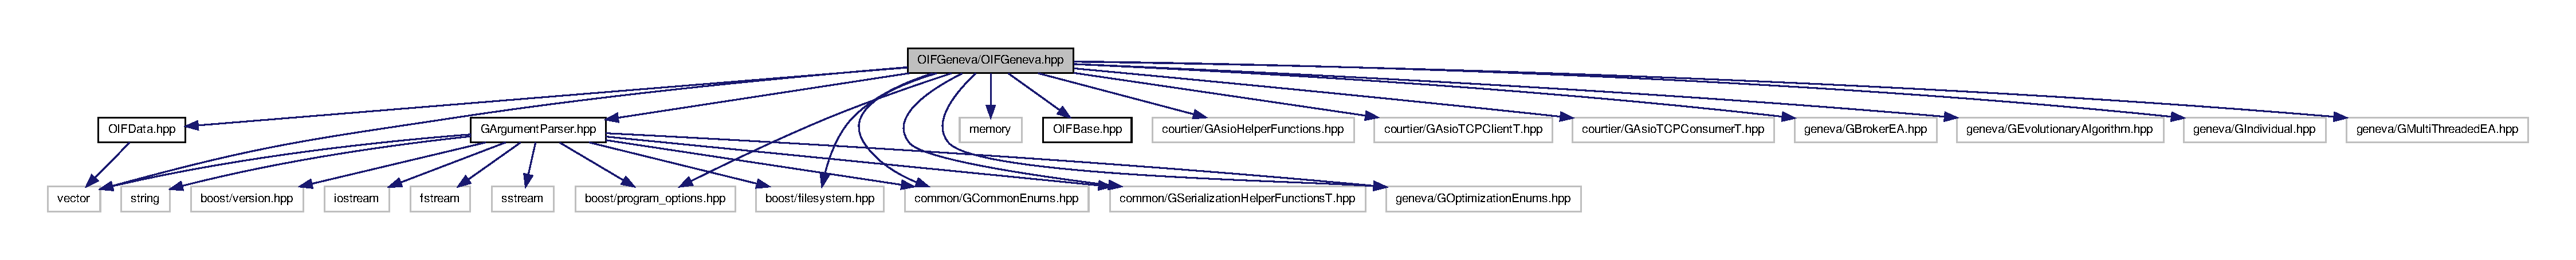
\includegraphics[width=400pt]{d9/df0/OIFGeneva_8hpp__incl}
\end{center}
\end{figure}
This graph shows which files directly or indirectly include this file:
\nopagebreak
\begin{figure}[H]
\begin{center}
\leavevmode
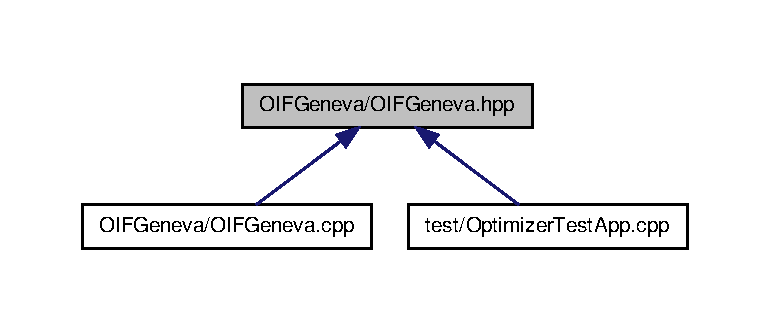
\includegraphics[width=370pt]{d5/d3f/OIFGeneva_8hpp__dep__incl}
\end{center}
\end{figure}
\subsection*{Classes}
\begin{DoxyCompactItemize}
\item 
class \hyperlink{classOIFGeneva}{OIFGeneva}
\begin{DoxyCompactList}\small\item\em Wrapper of the Geneva Optimizer library. \end{DoxyCompactList}\end{DoxyCompactItemize}


\subsection{Detailed Description}
This class provides a wrapper around the Geneva library. It fulfills the \hyperlink{classOIFBase}{OIFBase} interface to be easily adapted to other modules. Parameters for the optimization have to be provided in a config-\/file, the data needs to be provided with the \hyperlink{classOIFData}{OIFData} interface. 
\hypertarget{OIFMinuit_8cpp}{
\section{OIFMinuit2/OIFMinuit.cpp File Reference}
\label{d7/d2d/OIFMinuit_8cpp}\index{OIFMinuit2/OIFMinuit.cpp@{OIFMinuit2/OIFMinuit.cpp}}
}
{\ttfamily \#include $<$vector$>$}\par
{\ttfamily \#include $<$string$>$}\par
{\ttfamily \#include $<$sstream$>$}\par
{\ttfamily \#include $<$iostream$>$}\par
{\ttfamily \#include $<$memory$>$}\par
{\ttfamily \#include \char`\"{}Minuit2/MnUserParameters.h\char`\"{}}\par
{\ttfamily \#include \char`\"{}Minuit2/MnMigrad.h\char`\"{}}\par
{\ttfamily \#include \char`\"{}Minuit2/FunctionMinimum.h\char`\"{}}\par
{\ttfamily \#include \char`\"{}Minuit2/MnMinos.h\char`\"{}}\par
{\ttfamily \#include \char`\"{}Minuit2/MnStrategy.h\char`\"{}}\par
{\ttfamily \#include \char`\"{}OIFMinuit.hpp\char`\"{}}\par

\hypertarget{OIFMinuit_8hpp}{
\section{OIFMinuit2/OIFMinuit.hpp File Reference}
\label{d8/d0f/OIFMinuit_8hpp}\index{OIFMinuit2/OIFMinuit.hpp@{OIFMinuit2/OIFMinuit.hpp}}
}


This class provides a wrapper around the Minuit2 library.  


{\ttfamily \#include $<$vector$>$}\par
{\ttfamily \#include $<$memory$>$}\par
{\ttfamily \#include \char`\"{}OIFData.hpp\char`\"{}}\par
{\ttfamily \#include \char`\"{}OIFBase.hpp\char`\"{}}\par
{\ttfamily \#include \char`\"{}OIFMinuitFcn.hpp\char`\"{}}\par
\subsection*{Classes}
\begin{DoxyCompactItemize}
\item 
class \hyperlink{classOIFMinuit}{OIFMinuit}
\begin{DoxyCompactList}\small\item\em Wrapper of the Minuit2 Optimizer library. \end{DoxyCompactList}\end{DoxyCompactItemize}


\subsection{Detailed Description}
This class provides a wrapper around the Minuit2 library. It fulfills the \hyperlink{classOIFBase}{OIFBase} interface to be easily adapted to other modules. The data needs to be provided with the \hyperlink{classOIFData}{OIFData} interface. 
\hypertarget{OIFMinuitFcn_8cpp}{
\section{OIFMinuit2/OIFMinuitFcn.cpp File Reference}
\label{d5/db0/OIFMinuitFcn_8cpp}\index{OIFMinuit2/OIFMinuitFcn.cpp@{OIFMinuit2/OIFMinuitFcn.cpp}}
}
{\ttfamily \#include \char`\"{}OIFMinuitFcn.hpp\char`\"{}}\par
{\ttfamily \#include \char`\"{}OIFData.hpp\char`\"{}}\par
{\ttfamily \#include \char`\"{}PWAParameter.hpp\char`\"{}}\par
{\ttfamily \#include $<$cassert$>$}\par
{\ttfamily \#include $<$memory$>$}\par
{\ttfamily \#include $<$iostream$>$}\par
Include dependency graph for OIFMinuitFcn.cpp:\nopagebreak
\begin{figure}[H]
\begin{center}
\leavevmode
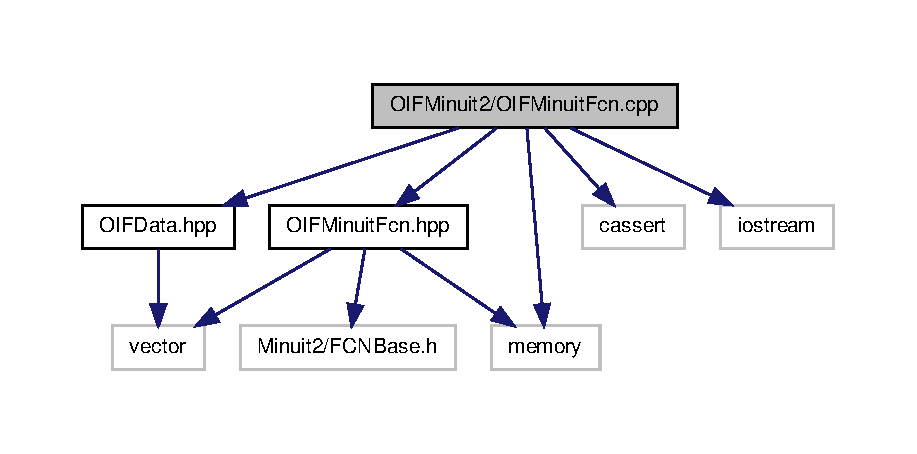
\includegraphics[width=400pt]{dd/d6f/OIFMinuitFcn_8cpp__incl}
\end{center}
\end{figure}

\hypertarget{OIFMinuitFcn_8hpp}{
\section{OIFMinuit2/OIFMinuitFcn.hpp File Reference}
\label{d4/dce/OIFMinuitFcn_8hpp}\index{OIFMinuit2/OIFMinuitFcn.hpp@{OIFMinuit2/OIFMinuitFcn.hpp}}
}


Based on the Minuit2 FcnBase.  


{\ttfamily \#include $<$vector$>$}\par
{\ttfamily \#include $<$memory$>$}\par
{\ttfamily \#include \char`\"{}Minuit2/FCNBase.h\char`\"{}}\par
Include dependency graph for OIFMinuitFcn.hpp:
\nopagebreak
\begin{figure}[H]
\begin{center}
\leavevmode
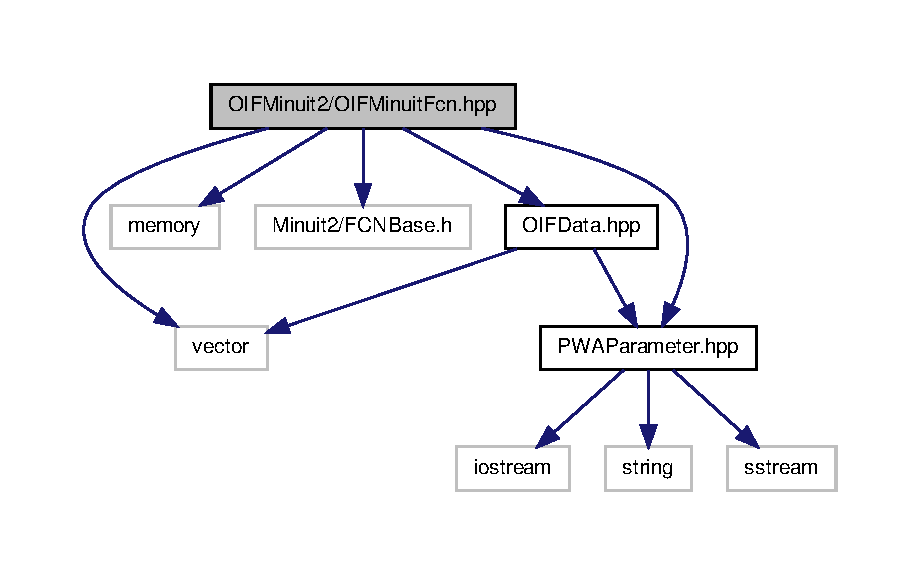
\includegraphics[width=314pt]{d1/d8e/OIFMinuitFcn_8hpp__incl}
\end{center}
\end{figure}
This graph shows which files directly or indirectly include this file:
\nopagebreak
\begin{figure}[H]
\begin{center}
\leavevmode
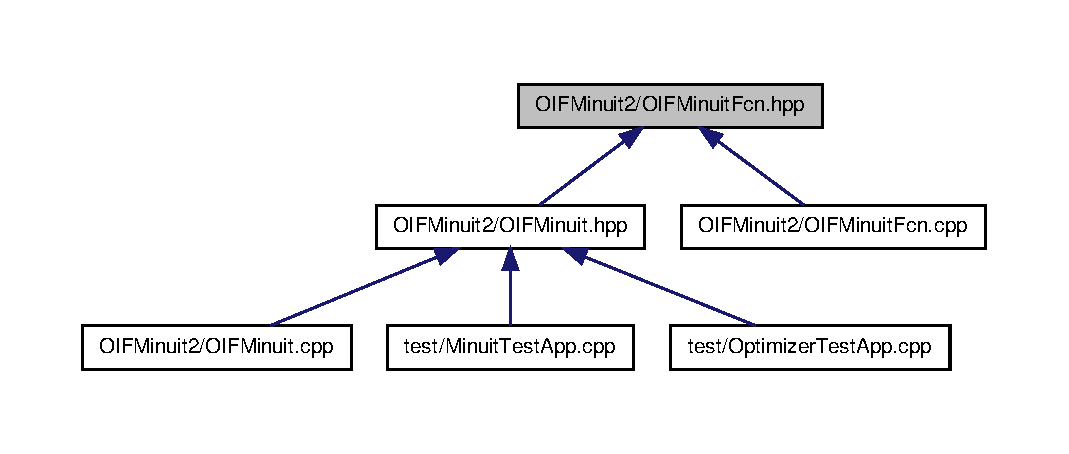
\includegraphics[width=400pt]{d3/da6/OIFMinuitFcn_8hpp__dep__incl}
\end{center}
\end{figure}
\subsection*{Classes}
\begin{DoxyCompactItemize}
\item 
class \hyperlink{classROOT_1_1Minuit2_1_1OIFMinuitFcn}{ROOT::Minuit2::OIFMinuitFcn}
\end{DoxyCompactItemize}
\subsection*{Namespaces}
\begin{DoxyCompactItemize}
\item 
namespace \hyperlink{namespaceROOT}{ROOT}
\item 
namespace \hyperlink{namespaceROOT_1_1Minuit2}{ROOT::Minuit2}
\end{DoxyCompactItemize}


\subsection{Detailed Description}
Based on the Minuit2 FcnBase. This class uses the \hyperlink{classOIFData}{OIFData} interface for the optimization. 
\hypertarget{PIFBW_8cpp}{
\section{PIFBW/PIFBW.cpp File Reference}
\label{d5/dbb/PIFBW_8cpp}\index{PIFBW/PIFBW.cpp@{PIFBW/PIFBW.cpp}}
}
{\ttfamily \#include $<$vector$>$}\par
{\ttfamily \#include $<$string$>$}\par
{\ttfamily \#include $<$sstream$>$}\par
{\ttfamily \#include $<$iostream$>$}\par
{\ttfamily \#include \char`\"{}PIFBW.hpp\char`\"{}}\par
Include dependency graph for PIFBW.cpp:
\nopagebreak
\begin{figure}[H]
\begin{center}
\leavevmode
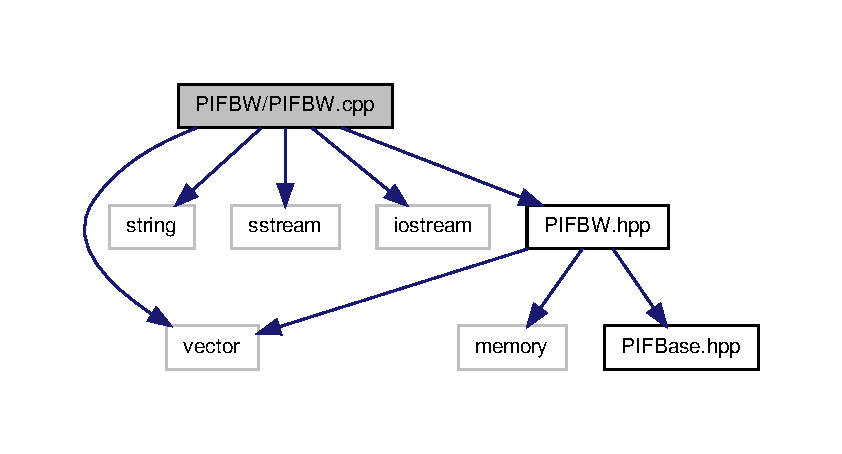
\includegraphics[width=400pt]{dc/de6/PIFBW_8cpp__incl}
\end{center}
\end{figure}

\hypertarget{PIFBW_8hpp}{
\section{PIFBW/PIFBW.hpp File Reference}
\label{dd/da0/PIFBW_8hpp}\index{PIFBW/PIFBW.hpp@{PIFBW/PIFBW.hpp}}
}


This class provides a simple Breit-\/Wigner calculation with given parameters.  


{\ttfamily \#include $<$vector$>$}\par
{\ttfamily \#include $<$memory$>$}\par
{\ttfamily \#include \char`\"{}PIFBase.hpp\char`\"{}}\par
Include dependency graph for PIFBW.hpp:\nopagebreak
\begin{figure}[H]
\begin{center}
\leavevmode
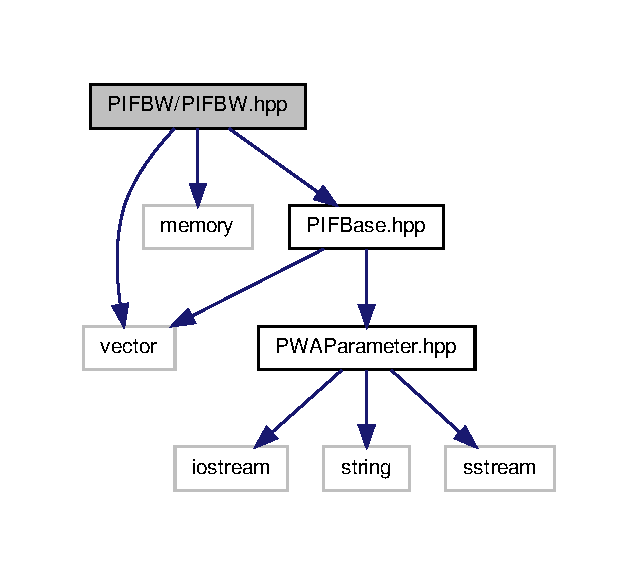
\includegraphics[width=306pt]{d4/d47/PIFBW_8hpp__incl}
\end{center}
\end{figure}
This graph shows which files directly or indirectly include this file:
\nopagebreak
\begin{figure}[H]
\begin{center}
\leavevmode
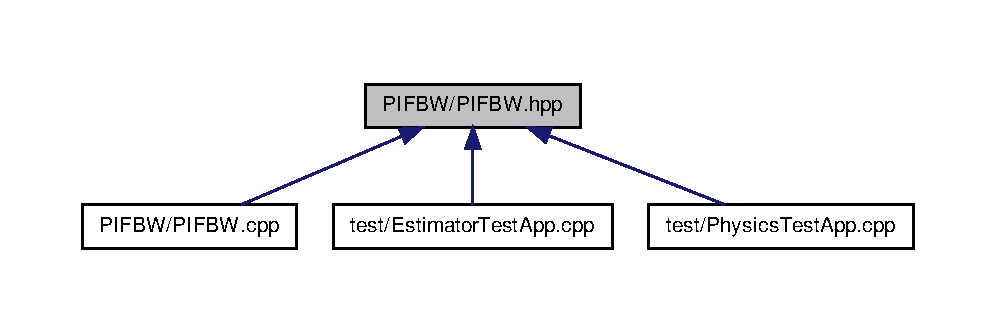
\includegraphics[width=400pt]{d4/dbe/PIFBW_8hpp__dep__incl}
\end{center}
\end{figure}
\subsection*{Classes}
\begin{DoxyCompactItemize}
\item 
class \hyperlink{classPIFBW}{PIFBW}
\begin{DoxyCompactList}\small\item\em Physics Module with simple 1D Breit-\/Wigner. \end{DoxyCompactList}\end{DoxyCompactItemize}


\subsection{Detailed Description}
This class provides a simple Breit-\/Wigner calculation with given parameters. It fulfills the \hyperlink{classPIFBase}{PIFBase} interface to be compatible with other ComPWA modules. 
\hypertarget{CX0TestApp_8cpp}{
\section{test/CX0TestApp.cpp File Reference}
\label{d5/d7b/CX0TestApp_8cpp}\index{test/CX0TestApp.cpp@{test/CX0TestApp.cpp}}
}


Test-\/Application to check c++11 support.  


{\ttfamily \#include $<$iostream$>$}\par
{\ttfamily \#include $<$memory$>$}\par
Include dependency graph for CX0TestApp.cpp:
\nopagebreak
\begin{figure}[H]
\begin{center}
\leavevmode
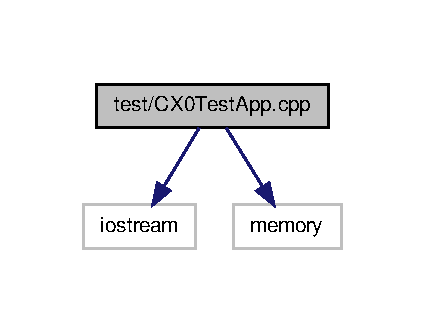
\includegraphics[width=204pt]{db/d23/CX0TestApp_8cpp__incl}
\end{center}
\end{figure}
\subsection*{Functions}
\begin{DoxyCompactItemize}
\item 
int \hyperlink{CX0TestApp_8cpp_a3c04138a5bfe5d72780bb7e82a18e627}{main} (int argc, char $\ast$$\ast$argv)
\end{DoxyCompactItemize}


\subsection{Detailed Description}
Test-\/Application to check c++11 support. This tiny application test some features of the new c++11 standard. One can compile and run this to check the c++11 support of the used compiler/system. 

\subsection{Function Documentation}
\hypertarget{CX0TestApp_8cpp_a3c04138a5bfe5d72780bb7e82a18e627}{
\index{CX0TestApp.cpp@{CX0TestApp.cpp}!main@{main}}
\index{main@{main}!CX0TestApp.cpp@{CX0TestApp.cpp}}
\subsubsection[{main}]{\setlength{\rightskip}{0pt plus 5cm}int main (
\begin{DoxyParamCaption}
\item[{int}]{argc, }
\item[{char $\ast$$\ast$}]{argv}
\end{DoxyParamCaption}
)}}
\label{d5/d7b/CX0TestApp_8cpp_a3c04138a5bfe5d72780bb7e82a18e627}

\hypertarget{DataIFTestApp_8cpp}{
\section{test/DataIFTestApp.cpp File Reference}
\label{db/d8a/DataIFTestApp_8cpp}\index{test/DataIFTestApp.cpp@{test/DataIFTestApp.cpp}}
}


Test-\/Application of the Root Data-\/IF.  


{\ttfamily \#include $<$iostream$>$}\par
{\ttfamily \#include $<$cmath$>$}\par
{\ttfamily \#include $<$sstream$>$}\par
{\ttfamily \#include $<$vector$>$}\par
{\ttfamily \#include $<$string$>$}\par
{\ttfamily \#include $<$memory$>$}\par
{\ttfamily \#include \char`\"{}TLorentzVector.h\char`\"{}}\par
{\ttfamily \#include \char`\"{}TH1D.h\char`\"{}}\par
{\ttfamily \#include \char`\"{}TFile.h\char`\"{}}\par
{\ttfamily \#include \char`\"{}DIFRootReader.hpp\char`\"{}}\par
{\ttfamily \#include \char`\"{}PWAEvent.hpp\char`\"{}}\par
{\ttfamily \#include \char`\"{}PWAParticle.hpp\char`\"{}}\par
Include dependency graph for DataIFTestApp.cpp:\nopagebreak
\begin{figure}[H]
\begin{center}
\leavevmode
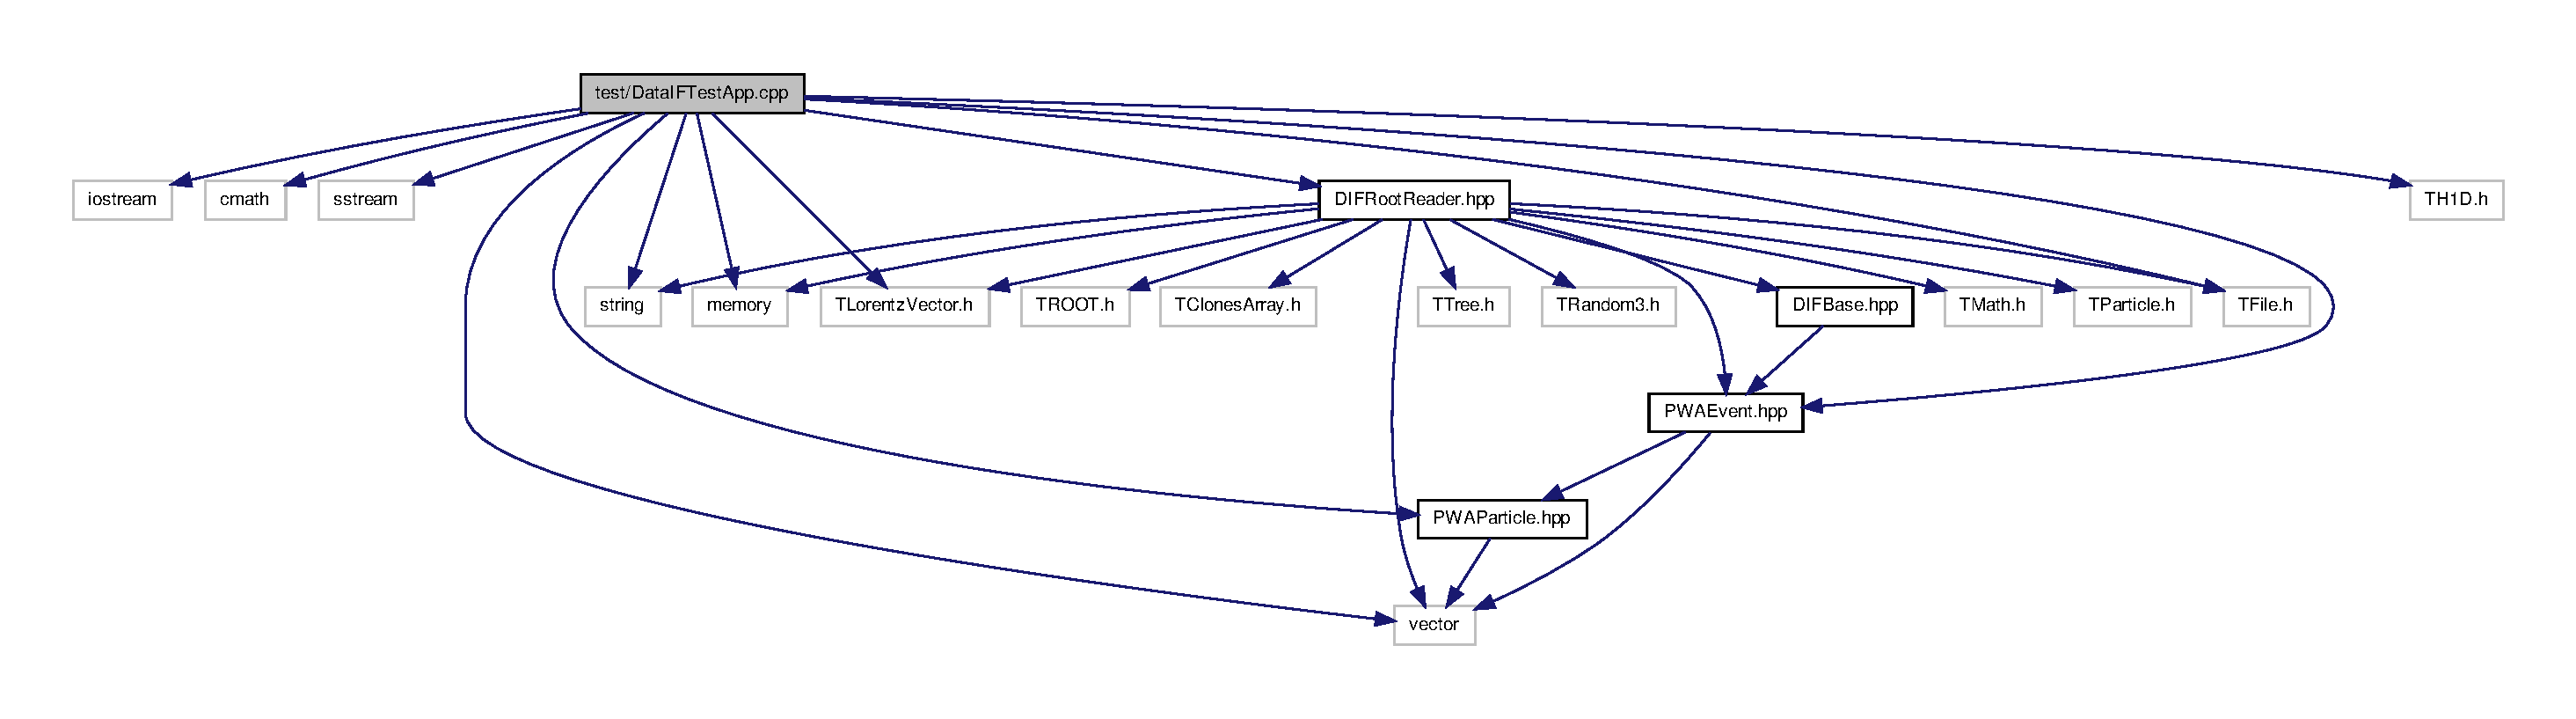
\includegraphics[width=400pt]{d2/d09/DataIFTestApp_8cpp__incl}
\end{center}
\end{figure}
\subsection*{Functions}
\begin{DoxyCompactItemize}
\item 
int \hyperlink{DataIFTestApp_8cpp_a3c04138a5bfe5d72780bb7e82a18e627}{main} (int argc, char $\ast$$\ast$argv)
\end{DoxyCompactItemize}


\subsection{Detailed Description}
Test-\/Application of the Root Data-\/IF. This tiny application tests the Root-\/format Data-\/IF. It reads a root file, plots the invariant mass of the first two particles and writes the result as well to another root file. 

\subsection{Function Documentation}
\hypertarget{DataIFTestApp_8cpp_a3c04138a5bfe5d72780bb7e82a18e627}{
\index{DataIFTestApp.cpp@{DataIFTestApp.cpp}!main@{main}}
\index{main@{main}!DataIFTestApp.cpp@{DataIFTestApp.cpp}}
\subsubsection[{main}]{\setlength{\rightskip}{0pt plus 5cm}int main (
\begin{DoxyParamCaption}
\item[{int}]{argc, }
\item[{char $\ast$$\ast$}]{argv}
\end{DoxyParamCaption}
)}}
\label{db/d8a/DataIFTestApp_8cpp_a3c04138a5bfe5d72780bb7e82a18e627}
The main function. 
\hypertarget{EstimatorTestApp_8cpp}{
\section{test/EstimatorTestApp.cpp File Reference}
\label{d4/d31/EstimatorTestApp_8cpp}\index{test/EstimatorTestApp.cpp@{test/EstimatorTestApp.cpp}}
}


Test-\/Application of a simple $\chi^{2}$ estimator.  


{\ttfamily \#include $<$iostream$>$}\par
{\ttfamily \#include $<$cmath$>$}\par
{\ttfamily \#include $<$sstream$>$}\par
{\ttfamily \#include $<$vector$>$}\par
{\ttfamily \#include $<$string$>$}\par
{\ttfamily \#include $<$memory$>$}\par
{\ttfamily \#include \char`\"{}DIFRootReader.hpp\char`\"{}}\par
{\ttfamily \#include \char`\"{}PIFBW.hpp\char`\"{}}\par
{\ttfamily \#include \char`\"{}EIFChiOneD.hpp\char`\"{}}\par
{\ttfamily \#include \char`\"{}PWAParticle.hpp\char`\"{}}\par
{\ttfamily \#include \char`\"{}PWAParameter.hpp\char`\"{}}\par
Include dependency graph for EstimatorTestApp.cpp:\nopagebreak
\begin{figure}[H]
\begin{center}
\leavevmode
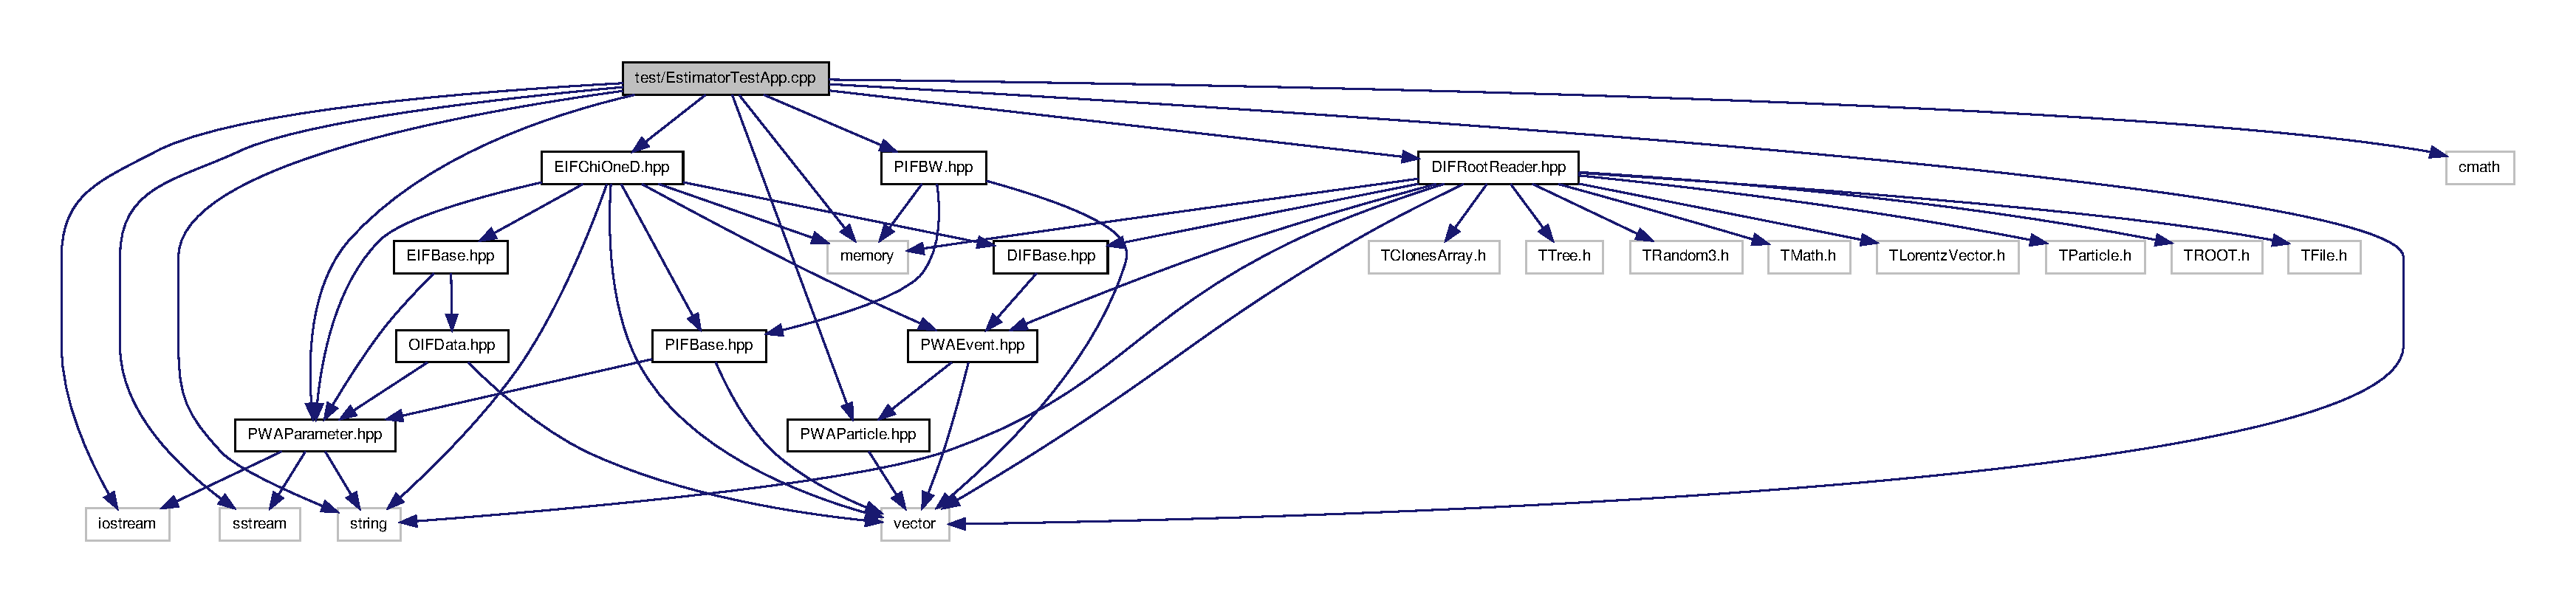
\includegraphics[width=400pt]{d9/d0d/EstimatorTestApp_8cpp__incl}
\end{center}
\end{figure}
\subsection*{Functions}
\begin{DoxyCompactItemize}
\item 
int \hyperlink{EstimatorTestApp_8cpp_a3c04138a5bfe5d72780bb7e82a18e627}{main} (int argc, char $\ast$$\ast$argv)
\end{DoxyCompactItemize}


\subsection{Detailed Description}
Test-\/Application of a simple $\chi^{2}$ estimator. This tiny application tests a simple $\chi^{2}$ estimator module. It reads data via the root-\/reader module \hyperlink{classDIFRootReader}{DIFRootReader},hpp and uses the intensity provided by the simple 1D-\/Breit-\/Wigner physics module \hyperlink{PIFBW_8hpp}{PIFBW.hpp}. As result it prints a calculated $\chi^{2}$ to the terminal. 

\subsection{Function Documentation}
\hypertarget{EstimatorTestApp_8cpp_a3c04138a5bfe5d72780bb7e82a18e627}{
\index{EstimatorTestApp.cpp@{EstimatorTestApp.cpp}!main@{main}}
\index{main@{main}!EstimatorTestApp.cpp@{EstimatorTestApp.cpp}}
\subsubsection[{main}]{\setlength{\rightskip}{0pt plus 5cm}int main (
\begin{DoxyParamCaption}
\item[{int}]{argc, }
\item[{char $\ast$$\ast$}]{argv}
\end{DoxyParamCaption}
)}}
\label{d4/d31/EstimatorTestApp_8cpp_a3c04138a5bfe5d72780bb7e82a18e627}
The main function. 
\hypertarget{IntegrationTestApp_8cpp}{
\section{test/IntegrationTestApp.cpp File Reference}
\label{d5/d26/IntegrationTestApp_8cpp}\index{test/IntegrationTestApp.cpp@{test/IntegrationTestApp.cpp}}
}


Test-\/Application for full fit with simple modules.  


{\ttfamily \#include $<$iostream$>$}\par
{\ttfamily \#include $<$cmath$>$}\par
{\ttfamily \#include $<$sstream$>$}\par
{\ttfamily \#include $<$vector$>$}\par
{\ttfamily \#include $<$string$>$}\par
{\ttfamily \#include $<$memory$>$}\par
{\ttfamily \#include \char`\"{}DIFRootReader.hpp\char`\"{}}\par
{\ttfamily \#include \char`\"{}PIFBW.hpp\char`\"{}}\par
{\ttfamily \#include \char`\"{}EIFChiOneD.hpp\char`\"{}}\par
{\ttfamily \#include \char`\"{}OIFMinuit.hpp\char`\"{}}\par
{\ttfamily \#include \char`\"{}PolyFit.hpp\char`\"{}}\par
Include dependency graph for IntegrationTestApp.cpp:\nopagebreak
\begin{figure}[H]
\begin{center}
\leavevmode
\includegraphics[width=400pt]{da/d03/IntegrationTestApp_8cpp__incl}
\end{center}
\end{figure}
\subsection*{Functions}
\begin{DoxyCompactItemize}
\item 
int \hyperlink{IntegrationTestApp_8cpp_a3c04138a5bfe5d72780bb7e82a18e627}{main} (int argc, char $\ast$$\ast$argv)
\end{DoxyCompactItemize}


\subsection{Detailed Description}
Test-\/Application for full fit with simple modules. This tiny application tests a simple fit procedure with a set of simple modules. It uses a simle $\chi^{2}$ estimator \hyperlink{classEIFChiOneD}{EIFChiOneD}, it reads data via the root-\/reader module \hyperlink{classDIFRootReader}{DIFRootReader} and uses the intensity provided by the simple 1D-\/Breit-\/Wigner physics module \hyperlink{classPIFBW}{PIFBW}. The optimization of the parameters is done with the Minuit2 module \hyperlink{classOIFMinuit}{OIFMinuit}. As result the optimized parameters are printed to the terminal. 

\subsection{Function Documentation}
\hypertarget{IntegrationTestApp_8cpp_a3c04138a5bfe5d72780bb7e82a18e627}{
\index{IntegrationTestApp.cpp@{IntegrationTestApp.cpp}!main@{main}}
\index{main@{main}!IntegrationTestApp.cpp@{IntegrationTestApp.cpp}}
\subsubsection[{main}]{\setlength{\rightskip}{0pt plus 5cm}int main (
\begin{DoxyParamCaption}
\item[{int}]{argc, }
\item[{char $\ast$$\ast$}]{argv}
\end{DoxyParamCaption}
)}}
\label{d5/d26/IntegrationTestApp_8cpp_a3c04138a5bfe5d72780bb7e82a18e627}
The main function. 
\hypertarget{MinuitTestApp_8cpp}{
\section{test/MinuitTestApp.cpp File Reference}
\label{da/d21/MinuitTestApp_8cpp}\index{test/MinuitTestApp.cpp@{test/MinuitTestApp.cpp}}
}


Test-\/Application of the Minuit2 Optimizer-\/IF.  


{\ttfamily \#include $<$iostream$>$}\par
{\ttfamily \#include $<$cmath$>$}\par
{\ttfamily \#include $<$sstream$>$}\par
{\ttfamily \#include $<$vector$>$}\par
{\ttfamily \#include $<$string$>$}\par
{\ttfamily \#include $<$memory$>$}\par
{\ttfamily \#include $<$boost/lexical\_\-cast.hpp$>$}\par
{\ttfamily \#include \char`\"{}OIFMinuit.hpp\char`\"{}}\par
{\ttfamily \#include \char`\"{}PolyFit.hpp\char`\"{}}\par
Include dependency graph for MinuitTestApp.cpp:
\nopagebreak
\begin{figure}[H]
\begin{center}
\leavevmode
\includegraphics[width=400pt]{d9/d21/MinuitTestApp_8cpp__incl}
\end{center}
\end{figure}
\subsection*{Functions}
\begin{DoxyCompactItemize}
\item 
int \hyperlink{MinuitTestApp_8cpp_a3c04138a5bfe5d72780bb7e82a18e627}{main} (int argc, char $\ast$$\ast$argv)
\end{DoxyCompactItemize}


\subsection{Detailed Description}
Test-\/Application of the Minuit2 Optimizer-\/IF. This tiny application tests the interface to the Minuit2 Optimizer. The test dataset is generated in the \hyperlink{PolyFit_8hpp}{PolyFit.hpp} class, which creates smeared 1-\/dim data according to a polynomial function. Then the Minuit2-\/IF is used to fit the same polynomial to the smeared points and as a result the optimized parameters are printed. 

\subsection{Function Documentation}
\hypertarget{MinuitTestApp_8cpp_a3c04138a5bfe5d72780bb7e82a18e627}{
\index{MinuitTestApp.cpp@{MinuitTestApp.cpp}!main@{main}}
\index{main@{main}!MinuitTestApp.cpp@{MinuitTestApp.cpp}}
\subsubsection[{main}]{\setlength{\rightskip}{0pt plus 5cm}int main (
\begin{DoxyParamCaption}
\item[{int}]{argc, }
\item[{char $\ast$$\ast$}]{argv}
\end{DoxyParamCaption}
)}}
\label{da/d21/MinuitTestApp_8cpp_a3c04138a5bfe5d72780bb7e82a18e627}
The main function. 
\hypertarget{OptimizerTestApp_8cpp}{
\section{test/OptimizerTestApp.cpp File Reference}
\label{d4/db7/OptimizerTestApp_8cpp}\index{test/OptimizerTestApp.cpp@{test/OptimizerTestApp.cpp}}
}


Test-\/Application of the Optimizer-\/IF.  


{\ttfamily \#include $<$iostream$>$}\par
{\ttfamily \#include $<$cmath$>$}\par
{\ttfamily \#include $<$sstream$>$}\par
{\ttfamily \#include $<$vector$>$}\par
{\ttfamily \#include $<$string$>$}\par
{\ttfamily \#include $<$memory$>$}\par
{\ttfamily \#include $<$boost/lexical\_\-cast.hpp$>$}\par
{\ttfamily \#include \char`\"{}OIFMinuit.hpp\char`\"{}}\par
{\ttfamily \#include \char`\"{}OIFGeneva.hpp\char`\"{}}\par
{\ttfamily \#include \char`\"{}PolyFit.hpp\char`\"{}}\par
Include dependency graph for OptimizerTestApp.cpp:
\nopagebreak
\begin{figure}[H]
\begin{center}
\leavevmode
\includegraphics[width=400pt]{d0/d6f/OptimizerTestApp_8cpp__incl}
\end{center}
\end{figure}
\subsection*{Functions}
\begin{DoxyCompactItemize}
\item 
int \hyperlink{OptimizerTestApp_8cpp_a3c04138a5bfe5d72780bb7e82a18e627}{main} (int argc, char $\ast$$\ast$argv)
\end{DoxyCompactItemize}


\subsection{Detailed Description}
Test-\/Application of the Optimizer-\/IF. This tiny application tests the interface to the Optimizers Minuit2 and Geneva. The test dataset is generated in the \hyperlink{PolyFit_8hpp}{PolyFit.hpp} class, which creates smeared 1-\/dim data according to a polynomial function. Then the Optimizer-\/IF implemen-\/ tations Minuit2 (\hyperlink{OIFMinuit_8hpp}{OIFMinuit.hpp}) and Geneva (\hyperlink{OIFGeneva_8hpp}{OIFGeneva.hpp}) are used one after the other to fit the same polynomial to the smeared points. As a result the optimized parameters are printed. Note: In this example Minuit2 uses the final parameters of Geneva as starting values! 

\subsection{Function Documentation}
\hypertarget{OptimizerTestApp_8cpp_a3c04138a5bfe5d72780bb7e82a18e627}{
\index{OptimizerTestApp.cpp@{OptimizerTestApp.cpp}!main@{main}}
\index{main@{main}!OptimizerTestApp.cpp@{OptimizerTestApp.cpp}}
\subsubsection[{main}]{\setlength{\rightskip}{0pt plus 5cm}int main (
\begin{DoxyParamCaption}
\item[{int}]{argc, }
\item[{char $\ast$$\ast$}]{argv}
\end{DoxyParamCaption}
)}}
\label{d4/db7/OptimizerTestApp_8cpp_a3c04138a5bfe5d72780bb7e82a18e627}
The main function. 
\hypertarget{ParameterTestApp_8cpp}{
\section{test/ParameterTestApp.cpp File Reference}
\label{de/d58/ParameterTestApp_8cpp}\index{test/ParameterTestApp.cpp@{test/ParameterTestApp.cpp}}
}


Test-\/Application of internal \hyperlink{classPWAParameter}{PWAParameter}.  


{\ttfamily \#include $<$iostream$>$}\par
{\ttfamily \#include $<$cmath$>$}\par
{\ttfamily \#include $<$sstream$>$}\par
{\ttfamily \#include $<$vector$>$}\par
{\ttfamily \#include $<$string$>$}\par
{\ttfamily \#include $<$memory$>$}\par
{\ttfamily \#include \char`\"{}PWAParameter.hpp\char`\"{}}\par
Include dependency graph for ParameterTestApp.cpp:\nopagebreak
\begin{figure}[H]
\begin{center}
\leavevmode
\includegraphics[width=400pt]{d4/d56/ParameterTestApp_8cpp__incl}
\end{center}
\end{figure}
\subsection*{Functions}
\begin{DoxyCompactItemize}
\item 
int \hyperlink{ParameterTestApp_8cpp_a3c04138a5bfe5d72780bb7e82a18e627}{main} (int argc, char $\ast$$\ast$argv)
\end{DoxyCompactItemize}


\subsection{Detailed Description}
Test-\/Application of internal \hyperlink{classPWAParameter}{PWAParameter}. This tiny application tests the ComPWA internal Parameter class \hyperlink{classPWAParameter}{PWAParameter}. 

\subsection{Function Documentation}
\hypertarget{ParameterTestApp_8cpp_a3c04138a5bfe5d72780bb7e82a18e627}{
\index{ParameterTestApp.cpp@{ParameterTestApp.cpp}!main@{main}}
\index{main@{main}!ParameterTestApp.cpp@{ParameterTestApp.cpp}}
\subsubsection[{main}]{\setlength{\rightskip}{0pt plus 5cm}int main (
\begin{DoxyParamCaption}
\item[{int}]{argc, }
\item[{char $\ast$$\ast$}]{argv}
\end{DoxyParamCaption}
)}}
\label{de/d58/ParameterTestApp_8cpp_a3c04138a5bfe5d72780bb7e82a18e627}
The main function. 
\hypertarget{PhysicsTestApp_8cpp}{
\section{test/PhysicsTestApp.cpp File Reference}
\label{db/da0/PhysicsTestApp_8cpp}\index{test/PhysicsTestApp.cpp@{test/PhysicsTestApp.cpp}}
}


Test-\/Application of the Physics-\/IF.  


{\ttfamily \#include $<$iostream$>$}\par
{\ttfamily \#include $<$cmath$>$}\par
{\ttfamily \#include $<$sstream$>$}\par
{\ttfamily \#include $<$vector$>$}\par
{\ttfamily \#include $<$string$>$}\par
{\ttfamily \#include $<$memory$>$}\par
{\ttfamily \#include \char`\"{}PIFBW.hpp\char`\"{}}\par
Include dependency graph for PhysicsTestApp.cpp:
\nopagebreak
\begin{figure}[H]
\begin{center}
\leavevmode
\includegraphics[width=400pt]{d4/d1a/PhysicsTestApp_8cpp__incl}
\end{center}
\end{figure}
\subsection*{Functions}
\begin{DoxyCompactItemize}
\item 
int \hyperlink{PhysicsTestApp_8cpp_a3c04138a5bfe5d72780bb7e82a18e627}{main} (int argc, char $\ast$$\ast$argv)
\end{DoxyCompactItemize}


\subsection{Detailed Description}
Test-\/Application of the Physics-\/IF. This tiny application tests the interface to the Physics-\/Module. The simple implementation using a 1-\/dim Breit-\/Wigner is used and the intensity at the mean of the distribution is printed. 

\subsection{Function Documentation}
\hypertarget{PhysicsTestApp_8cpp_a3c04138a5bfe5d72780bb7e82a18e627}{
\index{PhysicsTestApp.cpp@{PhysicsTestApp.cpp}!main@{main}}
\index{main@{main}!PhysicsTestApp.cpp@{PhysicsTestApp.cpp}}
\subsubsection[{main}]{\setlength{\rightskip}{0pt plus 5cm}int main (
\begin{DoxyParamCaption}
\item[{int}]{argc, }
\item[{char $\ast$$\ast$}]{argv}
\end{DoxyParamCaption}
)}}
\label{db/da0/PhysicsTestApp_8cpp_a3c04138a5bfe5d72780bb7e82a18e627}
The main function. 
\hypertarget{PolyFit_8cpp}{
\section{test/PolyFit.cpp File Reference}
\label{d5/d8b/PolyFit_8cpp}\index{test/PolyFit.cpp@{test/PolyFit.cpp}}
}
{\ttfamily \#include $<$getopt.h$>$}\par
{\ttfamily \#include $<$fstream$>$}\par
{\ttfamily \#include $<$sstream$>$}\par
{\ttfamily \#include $<$iostream$>$}\par
{\ttfamily \#include $<$string$>$}\par
{\ttfamily \#include \char`\"{}PolyFit.hpp\char`\"{}}\par
{\ttfamily \#include \char`\"{}TFile.h\char`\"{}}\par
{\ttfamily \#include \char`\"{}TMath.h\char`\"{}}\par
{\ttfamily \#include \char`\"{}TGraph.h\char`\"{}}\par
{\ttfamily \#include \char`\"{}TCanvas.h\char`\"{}}\par
{\ttfamily \#include \char`\"{}TRandom.h\char`\"{}}\par
{\ttfamily \#include \char`\"{}TF1.h\char`\"{}}\par
{\ttfamily \#include \char`\"{}TGraphErrors.h\char`\"{}}\par

\hypertarget{PolyFit_8hpp}{
\section{test/PolyFit.hpp File Reference}
\label{d2/dcb/PolyFit_8hpp}\index{test/PolyFit.hpp@{test/PolyFit.hpp}}
}


This class derives from \hyperlink{OIFData_8hpp}{OIFData.hpp}, the data-\/interface of the optimizers.  


{\ttfamily \#include $<$iostream$>$}\par
{\ttfamily \#include $<$fstream$>$}\par
{\ttfamily \#include $<$string$>$}\par
{\ttfamily \#include $<$vector$>$}\par
{\ttfamily \#include $<$map$>$}\par
{\ttfamily \#include $<$cassert$>$}\par
{\ttfamily \#include $<$memory$>$}\par
{\ttfamily \#include $<$boost/shared\_\-ptr.hpp$>$}\par
{\ttfamily \#include \char`\"{}TROOT.h\char`\"{}}\par
{\ttfamily \#include \char`\"{}OIFData.hpp\char`\"{}}\par
\subsection*{Classes}
\begin{DoxyCompactItemize}
\item 
class \hyperlink{classPolyFit}{PolyFit}
\begin{DoxyCompactList}\small\item\em Test implementation of \hyperlink{OIFData_8hpp}{OIFData.hpp}. \end{DoxyCompactList}\end{DoxyCompactItemize}


\subsection{Detailed Description}
This class derives from \hyperlink{OIFData_8hpp}{OIFData.hpp}, the data-\/interface of the optimizers. It represents a set of 1-\/dim data-\/points, which are created when instantiating this class using a polynomial and smearing the points with a gausian distri-\/ bution. It also provides a draw function to visualize the data-\/points. 
\printindex
\end{document}
